% arara: pdflatex
% arara: pdflatex
% arara: pdflatex

% options:
% thesis=B bachelor's thesis
% thesis=M master's thesis
% czech thesis in Czech language
% slovak thesis in Slovak language
% english thesis in English language
% hidelinks remove colour boxes around hyperlinks

\documentclass[thesis=B,czech,hidelinks]{FITthesis}[2019/03/21]

\newcommand{\shellcmd}[1]{\\\indent\indent\texttt{\footnotesize\# #1}\\}

\RequirePackage{pdfpages}

%===========================================================================================================
\usepackage{verbatim}
\usepackage{fancyvrb}
\usepackage{listings}
\lstdefinestyle{example}{ %
%language=[5.1]Lua,                % choose the language of the code
basicstyle=\scriptsize\ttfamily, % the size of the fonts that are used
numbers=none,                   % where to put the line-numbers
numberstyle=\tiny,      % the size of the fonts that are used for
stepnumber=1,                   % the step between two line-numbers.
numbersep=5pt,                  % how far the line-numbers are from the code
showspaces=false,               % show spaces adding particular underscores
showstringspaces=false,         % underline spaces within strings
showtabs=false,                 % show tabs within strings adding particular
frame=single,           % adds a frame around the code
tabsize=2,          % sets default tabsize to 2 spaces
captionpos=b,           % sets the caption-position to bottom
breaklines=true,        % sets automatic line breaking
breakatwhitespace=false,
%escapeinside={\%*}{*)},     % if you want to add a comment within your code
fancyvrb=true,
}
%===========================================================================================================

\usepackage[utf8]{inputenc} % LaTeX source encoded as UTF-8

% \usepackage{amsmath} %advanced maths
% \usepackage{amssymb} %additional math symbols

\usepackage{dirtree,xevlna} %directory tree visualisation

% % list of acronyms
% \usepackage[acronym,nonumberlist,toc,numberedsection=autolabel]{glossaries}
% \iflanguage{czech}{\renewcommand*{\acronymname}{Seznam pou{\v z}it{\' y}ch zkratek}}{}
% \makeglossaries

\newcommand{\tg}{\mathop{\mathrm{tg}}} %cesky tangens
\newcommand{\cotg}{\mathop{\mathrm{cotg}}} %cesky cotangens

% % % % % % % % % % % % % % % % % % % % % % % % % % % % % % 
% ODTUD DAL VSE ZMENTE
% % % % % % % % % % % % % % % % % % % % % % % % % % % % % % 

\department{Katedra počítačových systémů}
\title{Automatické rozpoznávání síťových zařízení a jejich závislostí}
\authorGN{Josef} %(křestní) jméno (jména) autora
\authorFN{Koumar} %příjmení autora
\authorWithDegrees{Josef Koumar} %jméno autora včetně současných akademických titulů
\author{Josef Koumar} %jméno autora bez akademických titulů
\supervisor{Ing. Tomáš Čejka, Ph.D.}
\acknowledgements{Děkuji svému vedoucímu Ing. Tomáši Čejkovi, Ph.D. za rady a vstřícnost. Dále děkuji své rodině a přátelům za podporu a pomoc při psaní této bakalářské práce. Zejména přátelům Marcelu Poláčkovi za odborné rady a Tereze Ausficírové za rady ohledně stylizace českého jazyka.}

\abstractCS{
Tato práce se zabývá návrhem a implementací PassiveAutodiscovery modulu, který získá informace o zařízeních a určí jejich role v síti. Je vytvořen pro existující síťový modulární systém NEMEA. Teoretická část práce obsahuje popis, jakým způsobem modul získává informace o zařízeních ze sítě a praktická část obsahuje návrh a implementaci vzniklého modulu. Výsledky testování potvrzují funkčnost a ukazují časovou a paměťovou náročnost celého modulu.

Uživatel díky PassiveAutodiscovery modulu získá základní informace o všech zařízeních komunikující na měřené síti, role zařízeních v této síti, závislosti mezi zařízeními a statistiky používání sítě.
}
\abstractEN{
This thesis is about design and implementation of the PassiveAutodiscovery module, which receives information about devices and determines their role in network. Module is designed for an existing network modular system NEMEA. The theoretical part contains a description of how the module obtains information about devices from the network and the practical part contains the design and implementation of the resulting module. The test results confirm functionality and show the time and memory demands of the whole module.

Thanks to PassiveAutodiscovery, the user receives basic information about all devices communicating on the measured network, the role of the user in this network, interconnection between devices and network statistics.
}

\placeForDeclarationOfAuthenticity{V~Praze}
\declarationOfAuthenticityOption{2} %volba Prohlášení (číslo 1-6)

\keywordsCS{NEMEA, autodiscovery, detekce zařízeních, role zařízení v síti, servery a klienti, analýza síťového provozu, pasivní analýza, CESNET, python }
\keywordsEN{NEMEA, autodiscovery, device detection, role of the device in the network, servers and clients, network traffic analyze, passive analyze, CESNET, python}

% \website{http://site.example/thesis} %volitelná URL práce, objeví se v tiráži - úplně odstraňte, nemáte-li URL práce


\begin{document}

% \newacronym{CVUT}{{\v C}VUT}{{\v C}esk{\' e} vysok{\' e} u{\v c}en{\' i} technick{\' e} v Praze}
% \newacronym{FIT}{FIT}{Fakulta informa{\v c}n{\' i}ch technologi{\' i}}



%===========================================================================================================
%===========================================================================================================
%===========================================================================================================
\begin{introduction}	%sem napište úvod Vaší práce
Analýza komunikace na síti je v dnešní době jedna z podstatných úloh každého monitorovacího systému a lze ji provádět různými způsoby podmíněnými konkrétním úkolem analýzy. V konkrétním případě bezpečnostní analýzy je cíl odhalit potencionálně škodlivou komunikaci, jako jsou neoprávněné přístupy k zařízením v síti. Dále může analýza podávat statistické informace o síti a provozu na ní nebo monitorování funkčnosti a vyhodnocování chyb způsobených konfigurací. 

Monitorování sítě a následná analýza dat, stejně jako bezpečnost obecně, jsou prostředky pro minimalizaci rizik a hrozeb. Ve většině případů firmu motivuje k implementování monitorování sítě či bezpečnosti případná ztráta při bezpečnostních událostech nebo ztráty způsobené výpadky sítě. Dále díky monitorování sítě může firma sledovat přístupy k jednotlivým částem v síti a tím kontrolovat zda fungují nasazené bezpečnostní politiky. To vše lze z monitorování sítě vyčíst. Rychle a efektivně lze vyčíst i další informace užitečné k dalšímu použití. 

Z komunikace na lokální síti lze vyčíst informace o zařízení, které danou komunikaci vysílá či přijímá. Analýza těchto informací nejen přiřadí komunikaci v síti danému zařízení, ale také může rozhodnout o roli zařízení v síti a vytvoření mapy závislostí mezi zařízeními. Takové informace jsou pro správce sítě či zaměstnavatele hodně důležité. Dozví se, jaká zařízení se v síti nacházejí a jak se různá zařízení chovají na síti, a na základě těchto informací můžou být zavedeny změny v síti pro zlepšení komunikačních možností nebo pro zvýšení bezpečnosti. V případě znalosti, že bezpečnostní kamera je jedno ze zařízení připojené k síti může pomoci správci sítě ke specifikování pravidel filtrování v síti, což zablokuje možnost, že by bezpečnostní kamera chovala nestandardně. Rozpoznávání zařízení může být také použito pro blokování přístupu specifickým zařízením. Dále může správce sítě výstup monitorování porovnat s dokumentací sítě a nalézt tak nesrovnalosti s předpokladem.
%\widowpenalty10000

Ještě podstatnější jsou tyto informace například pro nového správce sítě, který převzal síť po bývalém správci bez předání potřebných informací. Z analýzy pak dostane představu o tom, jaká zařízení na síti jsou, jak mezi sebou komunikují, jaké služby vyžadují a jaké služby sami poskytují. Zařízení, která služby poskytují, se nazývají servery a jsou v síti ze všech nejdůležitější, jelikož poskytují služby, které ostatní zařízení používají. Analýza pak rozhodne, jaká zařízení jsou servery, a vypíše o nich důležité informace. Mezi nejdůležitější informace patří zejména IP adresa, poskytované služby a seznam klientů.

V práci se budeme zabývat návrhem a implementací modulu pro open-source monitorovací systém NEMEA  \cite{NEMEA}, který disponuje těmito vlastnosti a tento modul následně otestujeme na reálně funkční síti.

%===============================================================================================
%Jaké oblasti se práce týká, k čemu jsou užitečné výsledky práce, jaký je přínos, co se vylepšilo nebo udělalo nového, motivace proč se na tomto tématu dělalo DŮLEŽITÉ: nepsat o tom, že je něco v zadání!!!! Všechny naše práce mají praktickou motivaci, dělat něco, co je potřeba co může fungovat v praxi, co může pomoct je mnohem důležitější než dělat něco jen kvůli absolvování studia a odevzdání zp podle zadání!!! Zadání “neopisovat”, soustředit se na obsah práce a činností.
%===============================================================================================
\end{introduction}
%===========================================================================================================
%===========================================================================================================
%===========================================================================================================
\chapter{Cíl práce}
Cílem této práce je vytvořit analyzér rozšířených síťových toků zvaných IP flowsIP flows (popsaných např. v \cite{flowmonitoring}), jehož výstupem bude seznam serverů poskytující služby, seznam zařízení vyžadující tyto služby a mapa závislostí mezi těmito dvěma seznamy. Pro tento účel vytvoříme modul pro již existující open-source monitorovací systém NEMEA \cite{NEMEA}. Tento modul nazveme PassiveAutodiscovery modul a bude následně volně dostupný ve veřejně dostupném repozitáři na github.com.

PassiveAutodiscovery modul bude schopen z vstupních IP flows získat potřebné informace pro rozhodování o roli zařízení v síti a následnému oštítkování jednoduchými štítky vystihujícími jeho role v síti. Mezi štítky patří třeba DHCP Server, DNS Server a File Server. 

Dále modul získá základní informace o jednotlivých zařízeních a z komunikace na síti zjistí závislosti mezi nimi na lokální síti. Tyto závislosti přehledně vypíše včetně služeb, které byly v jednotlivých závislostech požadovány respektive poskytovány, a počtu přenesených paketů. Tuto funkcionalitu provede i pro přístupy zařízení mimo lokální síť a taktéž získané informace přehledně vypíše. Následně informace o závislostech modul vykreslí v mapách závislostí. Nakonec je statisticky vyhodnotí a přehledně vypíše pomocí grafů. Tyto záznamy bude modul vhodně dlouhodobě uchovávat.

Zařízení je v lokálním segmentu sítě jednoznačně rozpoznatelné podle MAC adresy a v celé lokální síti rozpoznatelné podle IP adresy. V této práci rozebereme problém jednoznačného rozpoznání zařízení v síti a pokusíme se implementovat algoritmus, který by spolehlivě rozpoznal zda se jedná o stejné zařízení i v případě změny IP adresy.




%===========================================================================================================
%===========================================================================================================
%===========================================================================================================
\chapter{Existující relevantní programy a práce}
Tato kapitola se zabývá již existujícími řešeními problému vyhledávání zařízení v síti, výpisu informací o nich a hledání závislostí mezi nimi. Ke každému programu je popsán jeho způsob řešení tohoto problému a následně je srovnán s vyvíjeným modulem pro systém NEMEA.

Základní kategorizací programů je rozdělení na proprietární a open-source programy. Tedy zda za jejich používání jejich autor či společnost zodpovědná za jejich vytvoření požaduje peněžní odměnu či nikoliv. Vybral jsem z každé této kategorie nejvýznamnější monitorovací programy. 
    \section{Proprietární programy}
        \subsection{Cisco ISE}
        Cisco ISE (Cisco Identity Services Engine) \cite{CiscoISEO} je kritická komponenta zero-trust architektury, což je typ zabezpečení firemní sítě, ve které se po každém zařízení vyžaduje ověření \uv{totožnosti}. Cisco ISE umožňuje zautomatizování procesu ověřování \uv{totožnosti} zařízeních dle předepsaných politik dané firmy. 
        
        Aby tato komponenta mohla ověřit \uv{totožnost} zařízení musí jej nejdříve nalézt a zjistit o nich co nejvíce informací. Proto obsahuje funkcionalitu nazvanou Asset Visibility, která umožňuje profilování zařízení. Cisco ISE \cite{CiscoISED} nejdříve použije k profilování aktivní sondy a senzory zařízeních, kterými nasbírá data o zařízeních. U aktivních sond v konkrétním případě používá utilitu NMAP (Network Mapper). Dále k profilování používá i pasivní způsob monitorování, který zpracovává data generovaná zařízeními. Jakmile Cisco ISE získá informace o zařízeních porovná je s databází a dle politik v ní nastaví zařízením oprávnění v síti.
        
        V porovnání s naším vyvíjeným PassiveAutodiscovery modulem Cisco ISE vyhledává zařízení a informace o nich pouze pro účely zero-trust architektury. K profilování zařízení Cisco ISE používá zvolený typ analýzy. Lze nastavit komponentu tak, aby používala pouze pasivní způsob monitorování, při které spoléhá na použité protokoly stejně jako náš modul. Také v pasivní analýze nahlíží Cisco ISE do aplikační vrstvy TCP/IP modelu u specifických protokolů, jako jsou CDP (Cisco Discovery Protocol), SMB (Server Message Block) a další, k zpřesnění pasivní analýzy, kvůli tomu je přesnější než náš modul. PassiveAutodiscovery modul má navíc, ale vyhledávání závislostí a vykreslování grafů závislostí. Dále se liší konkrétním použitím získaných informací. Náš modul informace získává pro zjištění rolí zařízeních a závislostí mezi nimi. Cisco ISE informace využívá jako základní data pro zero-trust architekturu.
        
        \subsection{User Device Tracker}
        User Device Tracker je součástí Network Performance Monitoru, což je programová sada vytvořená firmou SolarWinds, která se zabývá vývojem programových řešení managementu sítí, monitorování sítí, managementu databází a IT bezpečností.
        
        User Device Tracker \cite{SolarWinds} je implementován pro automatické sledování zařízení a správu portů na síťových přepínačích (angl. switch). Jeho hlavní úlohou je nacházení zařízení či uživatelů na síti a spojovat je s konkrétními porty na konkrétním síťovém přepínači. Hledání provádí dle uživatelského jména, IP adresy nebo MAC adresy a s cílem zvýšit bezpečnost v síti. V programu je možné určitá zařízení či uživatele zařadit na whitelist a neupozorňovat na jejich aktivitu explicitně, pouze logovat z jakého portu jakého switche se naposledy připojili nebo zda jsou na něm zrovna aktivní a ostatní zařízení zařadit na takzvaný watch list a program pak na ně automaticky upozorní pokud se do sítě přihlásí. 
        
        Program dále umožní kooperaci se síťovými zařízeními, díky čemuž může administrátor vypínat porty přímo z programu a tím zamezit případným bezpečnostním útokům ze stran neznámých či podezřelých zařízení. 
        
        Tento proprietární program je spíše určen pro zabezpečení a management switchů a zařízení vyhledává s cílem informovat administrátora o připojení zařízení ke switchi na určitém jeho portu. I tak vypisuje o zařízení základní informace, jako například IP adresu, MAC adresu, výrobce síťová karty či čas poslední aktivity v síti, čímž se mírně přibližuje k našemu PassiveAutodiscovery modulu, který taktéž tyto informace o zařízení vypisuje, ale s úplně odlišným cílem rozpoznávat role zařízení v síti a hledání jeho závislostí. Celková sada Network Performance Monitor dokáže mapovat závislosti mezi zařízeními a ty potom vykreslovat do map, stejná funkcionalita je zařazena i do našeho modulu.
        
        \subsection{PRTG Network Monitor}
        PRTG Network Monitor \cite{PRTG} je monitorovací systém vytvořený firmou Peassler, která se zabývá vývojem monitorovacího software s cílem usnadnit administrátorům práci a zvýšit bezpečnost v jejich firmách.
        
        Umožňuje zachytávání paketů, diagnostiku sítě, vyhledání síťových zařízení v síti, zmapování sítě, optimalizaci sítě a monitorování firewallů, IP adres, VoIP služeb, LAN sítě, Wi-Fi připojení, aktivit a bezpečnosti. Z těchto funkcionalit nás nejvíce zajímá monitorování LAN sítě. 
        
        Monitorování LAN sítě umožní administrátorovi sledoval aktivitu na síti, včetně pracovních stanic, serverů, routerů či tiskáren. PRTG monitoruje LAN síť a odesílá upozornění na problémy s připojením, omezenou dostupnost nebo přetížený server.
        
        V článku \cite{PRTGDevice} se dozvíme způsob hledání zařízení v LAN síti PRTG Network Monitoru, které probíhá následujícím způsobem:
        \begin{enumerate}
            \item Po zadání IP rozsahu PRTG použije utilitu ping pro najití všech zařízení v zadaném rozsahu.
            \item Následně zjistí roli jednotlivých zařízení v síti za použití SNMP (Simple Network Management Protocol), WMI (Windows Management Instrumentation Remote Protocol) a dalších protokolů.
            \item Všechna nalezená zařízení jsou nakonec umístěna do takzvaného device tree (někdy devicetree), což je datová struktura popisující hardwarové komponenty počítače.
        \end{enumerate}
        
        PRTG hledá zařízení v síti a rozhoduje o jejich roli v síti aktivním přístupem, tedy interaguje se zařízením s cílem zjištěni o jaké zařízení se jedná, na rozdíl od našeho modulu, který všechny informace o zařízení získává pasivním posloucháním komunikace na síti. Dále je náš modul open-source, což je výhoda oproti proprietárnímu PRTG.
        \subsection{OpManager}
        OpManager je monitorovací systém od firmy ManageEngine, která je IT management divize mezinárodní firmy Zoho corporation. ManageEngine se soustředí na vývoj monitorovacích softwarů v oblasti IT managementu a má na svědomí přes 90 programových řešení v této problematice.
        
        Monitorovací systém nabízí velice mnoho funkcionalit, které se v převážné většině věnují managementu síťových zařízení a serverů. V konkrétních příkladech to jsou monitorovaní síťových rozhraní, dostupnosti služeb, hardware serverů a síťových zařízení či zátěže na síťové linky. Nejpodstatnější funkcionality OpManageru jsou pro naší práci Ethernet Monitor, LAN Monitor a Network Device Discovery. 
        
        \emph{Ethernet Monitor} \cite{OpManagerEthernet} provádí v OpManageru monitorování lokální sítě se soustředěním na Ethernetové porty (dále jen porty). Ke každému portu vypisuje zda je na něm připojeno aktivní zařízení, základní informace o připojeném zařízení, zejména IP adresu, a přenosovou statistiku odeslaných a přijatých síťových rámců. Tyto informace pro každý port se v OpManageru nazývají Snapshot page. 
        
        \emph{LAN Monitor} \cite{OpManagerLAN} v OpManageru má za úkol monitorovat LAN síť za účelem zvýšení dostupnosti, ale také provádí in-depth analýzu výkonu sítě. Za těmito účely monitoruje dostupnost jednotlivých zařízení, míru jejich komunikace na síti a vykresluje je do přehledové mapy zařízení. Dále umožňuje sledovat zvolený subnet LAN sítě pro evidenci jednou kategorizovaných zařízeních v daném subnetu a přehledně informace o nich vypisovat. 
        
        Vypisuje o zařízeních například: 
        \begin{itemize}
            \item\emph{Status}  uvádí zda je v dané chvíli zařízení aktivní,
            \item\emph{IP adresu}  zařízení,
            \item\emph{Typ zařízení}  určuje operační systém zařízení a
            \item\emph{Kategorii}  upřesnující roli zařízení v síti.
        \end{itemize}
        OpManager vypíše všechny tyto informace s jistotou jen pokud byl na daný subnet předtím spuštěn Network Device Discovery popsaný dále. 
        
        V článku \cite{OpManagerNDD} se dočteme, že \emph{Network Device Discovery} pomáhá nalézat a sbírat informace o zařízeních jako jsou routery, switche, koncová zařízení neboli hosti a firewally. Dále také poskytuje mapování závislostí mezi těmito zařízeními. Nacházení zařízení probíhá stejným aktivním způsobem jako u PRTG Network Monitoru. 
        
        Tento program se v mnohých ohledech podobá PRTG Network Monitoru. Na rozdíl od našeho modulu provádí OpManager jednorázově nacházení zařízení aktivním způsobem při spuštění Network Device Discovery funkcionality, ale při běhu LAN Monitoru se provádí, jako u našeho modulu, také pasivní analýza, která buď doplňuje předešlou jednorázovou aktivní analýzu nebo je jediným zdrojem u nově připojených zařízeních.
    \section{Open-source programy}
    
        \subsection{Cacti}
        Cacti \cite{Cacti} je volně šiřitelný kompletně frontendový RRDTool, což je typ programu, který získává informace typu šířka pásma, teplota hardware a CPU load a ukládá je do databáze s časovou závislostí. Zároveň Cacti umožňuje další funkcionality jako dotazovací služby, pokročilé přizpůsobitelné grafy či management uživatelů. 
        
       Program lze nastavit tak, aby přímo sbíral data a základní konfiguraci RRDTool zakázat. Umožňuje navíc vkládat vlastní skripty na sbírání a práci s daty. Pro naše účely je nejzajímavější možnost hledání zařízení v síti, která v Cacti funguje následovně:
        \begin{enumerate}
            \item Použije SNMP nebo vlastní skript uživatele ke shromažďovaní dat o zařízení.
            \item Z informací sestaví inventář síťových zařízení.
            \item Inventář aktualizuje díky periodicky posílaným SNMP zprávám.
        \end{enumerate}
        
        Cacti je open-source program, který je primárně zaměřen na funkcionality RRDTool a díky otevřenosti a vkládání vlastních skriptů pro něj komunita vytvořila množství různorodých skriptů analyzující síť. V porovnání s naším modulem se Cacti soustředí na jinou oblast monitorování a na naší oblast vyhledávání a přiřazování rolí zařízením se nespecializuje, ale vytvořili jednoduchý funkční podprogram, který aktivním způsobem získává data o zařízeních a periodicky tuto aktivitu opakuje pro aktuálnost dat.
        
        \subsection{Zenmap}
        Zenmap \cite{Zenmap} je grafický scaner programu Nmap. Nmap je open-source program vyvíjený Gordonem Lyonem známým pod přezdívkou Fyodor. 
        
        Zenmap respektivě Nmap aktivně interaguje na síti s cílem najít zařízení a posbírat informace o nich, zejména otevřené porty na transportní vrstvě TCP/IP modelu, ze kterých usuzuje jaké služby dané zařízení v síti zprostředkovává. Tato činnost se provádí jednorázově na pokyn uživatele a výstup o zařízeních a jejich závislostech je přímo závislý na aktivních zařízeních v síti v daný moment. 
        
        O zařízeních dokáže vypsat:
        \begin{itemize}
            \item IP a MAC adresu,
            \item operační systém,
            \item otevřené porty a
            \item poslední boot.
        \end{itemize}
        
        Zenmap \cite{Zenmap} je jednorázový aktivní analyzér sítě, která najde v zadaném subnetu všechny v daný moment aktivní zařízení a ty následně podrobí analýze otevřených portů. Oproti našemu modulu se liší v aktivním analyzování sítě, nenachází závislosti mezi zařízeními, nevypisuje statistické údaje o provozu na síti a nevykresluje grafy závislostí. Přesto je to výborný nástroj pro rychlou analýzu aktivních zařízení v síti.
        
        \subsection{Spiceworks}
        Spiceworks \cite{Spiceworks} je monitorovací nástroj, který není open-source, ale za jeho používaní se nemusí platit, protože jeho vývoj je sponzorovaný reklamou v monitorovacím nástroji. Jeden z jeho produktů podporuje operace zajímavé pro naši práci. Spiceworks Inventory podporuje Network Discovery and Mapping funkcionalitu. 
        
        Tato funkcionalita proskenuje síť za účelem získání informací o připojených zařízeních. Pro tento účel používá utility Ping a NMAP. Na základě vytěžených dat vytvoří inventář zařízení a mapu sítě, přičemž o každém zařízení eviduje základní informace jako jsou IP adresa, MAC adresa, Operační systém a další. 
        
        Tato utilita monitorovacího nástroje Spiceworks jako ostatní již zmíněné spoléhá na aktivní interakci se sítí přičemž vypisuje základní informace, vykresluje mapu sítě a vytváří statistiky o používání sítě. Náš modul taktéž vypisuje informace o zařízeních a statistiky o síti, ale primárně je určen pro klasifikování role zařízení v síti. Spiceworks se pokouší vykreslovat reálnou mapu sítě, zatímco náš modul se soustředí na vykreslování mapu závislostí mezi zařízeními.
        
    \section{Pozorování}
    Všechny zmíněné monitorovací nástroje či systémy spoléhají primárně na aktivní interakci v síti. Čímž získají rychleji přesnější údaje o zařízeních připojených a zapnutých na síti. Zatímco náš modul spoléhá na pasivní monitorování komunikace na síti, ze které zjišťuje všechny informace. Výhodou těchto programů je rychlost a přesnost získání dat o zařízeních, ale za cenu zatěžování linek dotazy na jednotlivá zařízení, čímž se do jisté míry snižuje propustnost v síti. Výhoda našeho vyvíjeného PassiveAutodiscovery modulu pro modulární systém NEMEA je, že svojí činností neomezuje propustnost v síti a nevýhodou je, že aby zjistil informace o konkrétním zařízení musí dané zařízení vygenerovat potřebnou komunikaci na síti. 
        
%existující projekty nebo řešení a jak se liší nebo podobá naše zp, co je lepší a co horší, co bylo potřeba v praxi oproti existujícímu řešení
%===========================================================================================================
%===========================================================================================================
%===========================================================================================================
\chapter{Vyhledávání zařízení a určení jejich rolí v síti}
    Tato kapitola se bude zabývat existujícími dvěma způsoby vyhledávání zařízeních na síti a získaní informací o nich. Jsou to aktivní a pasivní způsob.
    
    V článku \cite{Passive} se dočteme, že při aktivním způsobu analyzér -- hardwarové zařízení či program nainstalovaný na počítači -- zahájí komunikaci na síti vysláním síťových rámců směrem k jednotlivým zařízením na síti. Ve většině případů se takovému analyzéru zadá rozsah síťového subnetu, na kterém se nacházejí cílová zařízení pro analyzování. Tento subnet pak zařízení či program projde a na každou IP adresu z rozsahu pošle krátkou zprávu typicky protokolem ICMP, a pokud se na dané IP adrese nachází aktivní zařízení, odpoví na tuto zprávu, čímž se analyzér dozví o aktivním zařízení na dané IP adrese. Poté se na nalezená zařízení vysílají další rámce obsahující zprávy, z jejichž odpovědí se analyzér dozví potřebné informace jako IP adresu, porty, služby, časové informace a informace o operačním systému zařízení. 
    
    Pasivní způsob analýzy, jak jsme se dočetli v článku \cite{Passive}, většinou nijak nekomunikuje na síti. Analyzér naslouchá běžné komunikaci na síti a z ní získává informace. Pokud na síti proběhne daná komunikace, tak jsou informace z ní téměř shodné s aktivním způsobem. Pasivní způsob umožňuje oproti aktivnímu způsobu získání informací o závislostech mezi zařízeními a jejich chování v síti. Dále je výhodou pasivního způsobu, že nezatěžuje síťové linky komunikací směrem k zařízením. A díky závislostem a chování zařízení v síti dokáže pasivní způsob mnohdy identifikovat zabezpečovací brány (angl. firewall), síťové směrovače (angl. router) či síťové přepínače (angl. switch) a při provedení NAT (Network Address Translation) potencionálně charakterizovat zařízení za nimi. Limitací pasivního způsobu je umístění analyzéru na síti. Musíme vždy rozhodovat kam umístit analyzér na základě informací, které chceme získat ze sítě. Této problematice se budeme v práci hlouběji zabývat v samostatné kapitole. Pasivní analýza může být použita například na zjištění běžného chování zařízení v síti, prosazování politik na síti, detekování hrozeb a monitorování událostí. 
    
    \begin{figure}
        \centering
        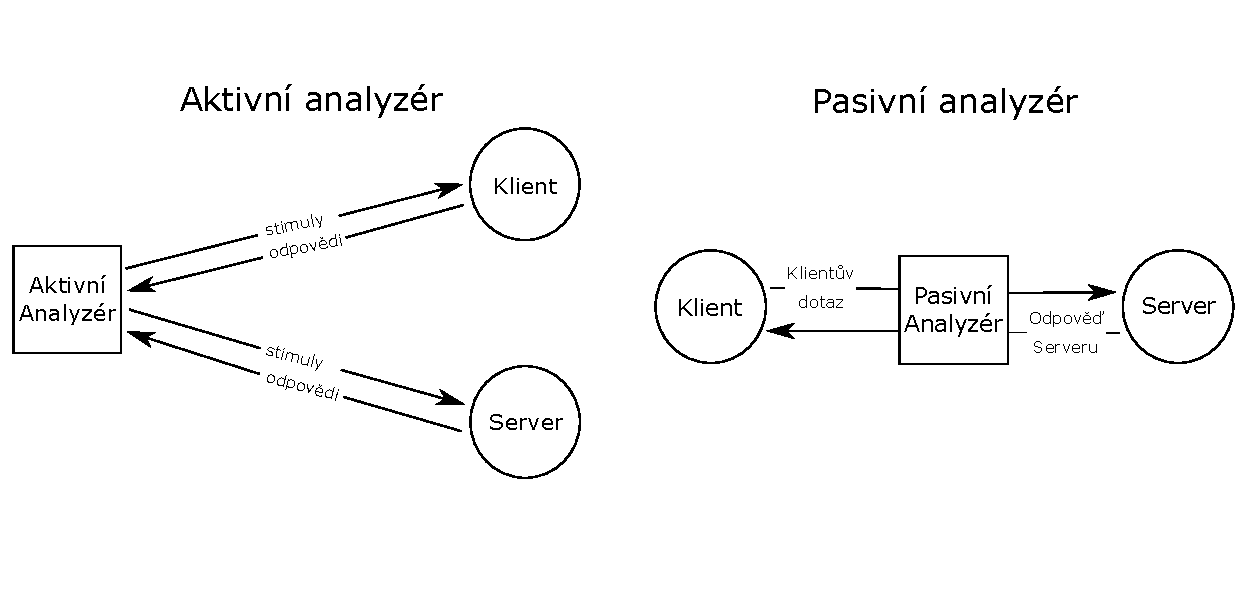
\includegraphics[width=\textwidth]{Active_Passive.pdf}
        \caption[Aktivní vs. pasivní analýza]{Aktivní vs. pasivní analýza}
        \label{PassiveVSAcite}
    \end{figure}
    
    V našem případě použijeme pasivní způsob analýzy zejména na získání základních informací o zařízeních, zjištění jejich rolí v (lokální) síti a závislostí mezi nimi. Nyní si popíšeme, jak toho docílíme.
    \section{Základní informace o zařízení}
    Mnohdy je spekulativní, co je to základní informace o zařízení. Pro tuto práci to však bude IP adresa zařízení, kterou uživatel může nastavit staticky nebo získat ze sítě dynamicky, čas poslední komunikace na síti, MAC adresa jeho síťové karty, kterou má většinou přidělenou od výrobce (v dnešní době lze MAC adresu změnit), a vendor, tedy výrobce síťové karty. Tyto informace jsou v každé komunikaci, která na síti probíhá. 
    
    Síťová a koncová zařízení jsou spojena dohromady pomocí různých typů médií, jako je kroucená dvoulinka a optické kabely. Po těchto médiích se komunikace převádí ve formě signálů signalizujících vždy binární hodnotu nuly nebo jedničky. Dohromady tyto bity vyslané do sítě tvoří síťový rámec první linkové vrstvy TCP/IP modelu, který obsahuje hlavičku, tělo a patičku. V hlavičce je umístěna zejména zdrojová a cílová MAC adresa a v patičce je umístěn kontrolní součet pro tento rámec. Tělo rámce je tvořeno daty, kterými je paket síťové vrstvy TCP/IP modelu. Paket je tvořen hlavičkou a tělem. Hlavička obsahuje zejména zdrojovou a cílovou IP adresu a tělo obsahuje segment třetí transportní vrstvy TCP/IP modelu. V segmentu se taktéž nachází hlavička a tělo. Zde je v hlavičce zejména zdrojový a cílový port použitého protokolu. V těle jsou data čtvrté aplikační vrstvy TCP/IP modelu, jejichž formát záleží na použitém protokolu. Na Obrázku \ref{Encapsulation} je vyobrazeno, jak zapouzdření (popsaný proces) probíhá při odeslání dat uživatele po síti. Data z komunikace tedy získáme nahlížením do hlaviček datových formátů jednotlivých vrstev.
    
    
    \begin{figure}[h]
        \centering
        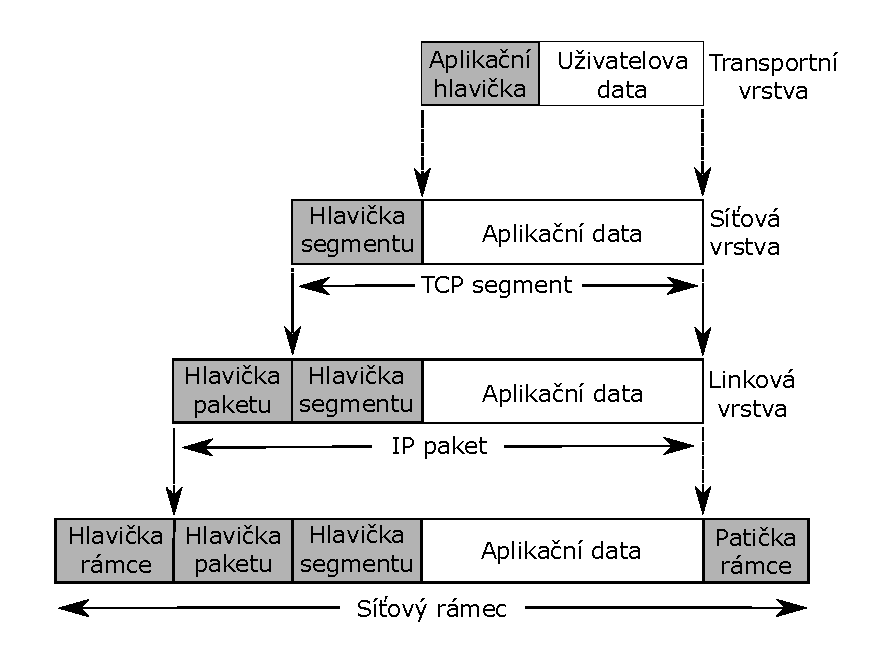
\includegraphics[width=\textwidth]{zapouzdreni.pdf}
        \caption[Zapouzdření]{Ukázka principu zapouzdření rámců v síťové komunikaci}
        \label{Encapsulation}
    \end{figure}
    
    V našem modulu se nepracuje přímo se síťovými rámci, nýbrž s flow záznamy, které se do našeho modulu dostanou z jiného již existujícího modulu. Ten vytvoří z rámců flow záznamy tak, že k rámci vyslanému ze zařízení přidá odpověď od druhého zařízení a takto vytvořený flow (biflow) odešle pomocí IFC rozhraní našemu modulu, který z něj pak získá snadněji informace ze všech hlaviček jednotlivých datových formátů popsaných vrstev. Výrobce síťového zařízení se pozná dle první poloviny MAC adresy, který je výrobcům přidělován.
    
    Pro získání všech těchto informací musí být monitorovací systém správně umístěn v síti. Pokud bychom třeba umístili náš modul za router mimo měřený segment lokální sítě, tak pro všechna zařízení, která náleží do tohoto segmentu, získáme stejnou MAC adresu a samozřejmě i vendora. Konkrétně to bude MAC adresa routeru, za nímž se segment sítě nachází. Více si o této problematice a způsobu řešení v našem modulu řekneme v následující kapitole.
    \section{Přiřazování štítků}
    Štítkováním nazveme proces, při kterém rozhodneme o roli zařízení v síti. Každou roli budeme reprezentovat štítkem, který tuto roli bude dostatečně specifikovat, a tento štítek následně přiřadíme k zařízení. Přičemž jedno zařízení může v síti mít více rolí. Například pokud zařízení bude poskytovat přístup k souborům přes síť, tak tomuto zařízení přiřadíme štítek \emph{File Server}.
    
    O roli budeme rozhodovat primárně z použitých protokolů v síťové komunikaci, jelikož většina protokolů se používá pro jeden specifický účel. Například protokol DHCP se v sítích používá výhradně na přidělování IP adres zařízením. Z předchozí kapitoly víme, že protokoly jsou v síťové komunikaci jednoznačně identifikované pomocí čísel portů v hlavičce segmentu na transportní vrstvě TCP/IP modelu. Z flow záznamů tedy stačí přečíst použité porty a ty následně porovnat se seznamem protokolů, které se používají pro specifické úlohy v síti. Pro tento účel vytvoříme tabulku, která bude tyto informace obsahovat.
    \begin{table}[h]
        \centering
        \caption{Rozdělení portů}
        \label{Ports}
        \begin{tabular}{|p{5cm}|c|p{4cm}|}\hline
            Název & Číselný rozsah & Popis \\\hline\hline
            Známé porty & 0 -- 1023 & dobře známé služby \\\hline
            Registrované porty & 1023 -- 49151 & registrované porty \\\hline
            Dynamické a soukromé porty & 49152 -- 65535 & běžné použití \\\hline
        \end{tabular}
    \end{table}
    
    Porty na transportní vrstvě přidělovala organizace IANA (Internet Assigned Numbers Authority) a od roku 2001 je touto funkcí pověřena organizace ICANN (Internet Corporation for Assigned Names and Numbers). Porty se rozdělují do tří skupin, jak je znázorněno v Tabulce \ref{Ports} \cite{IANA}.
    
    Nyní si projdeme nejpodstatnější role a popíšeme si jejich specifické protokoly, podle kterých je budeme rozpoznávat.
\subsection{Servery}
        Nejdůležitější zařízení v síti jsou bezpochyby servery, které poskytují ostatním zařízením služby, bez kterých by nemohli v síti fungovat. Existuje celá řada služeb, jenž můžou servery poskytovat. Tyto služby nyní identifikujeme a přiřadíme každé z nich štítek, jenž jí bude vystihovat. Obsah této sekce čerpá ze zdrojů \cite{IANA}, \cite{FILEP}, \cite{FILEtftp}, \cite{FILEnfs}, \cite{MAILP}, \cite{AuthentificateP}, \cite{Kerberos}, \cite{Radius}, a \cite{LDAPP}, které popisují jednotlivé použité protokoly.
        \begin{description}
            \item\emph{DHCP Server}  přiřazuje zařízením dynamicky IP adresy na základě protokolu DHCP, konkrétněji jeho verzí pro IPv4 a IPv6. 
            
            \item\emph{File Server}  poskytuje přístup k souborům přes síť, přičemž pro tuto funkcionalitu je možné používat celou řadu protokolů. Mezi nejpoužívanější zástupce těchto protokolů patří SMB (Server Message Block), NFS (Network File System) a TFTP (Trivial File Transfer Protocol). 
            
            \item\emph{Mail Server}  umožňuje posílání elektronických zpráv (e-mailů) přes síť. Základními protokoly pro tuto službu jsou IMAP (Internet Message Access Protocol), SMTP (Simple Mail Transfer Protocol) a POP (Post Office Protocol). Tyto protokoly mají více verzí včetně těch šifrovaných. 
            
            \item\emph{Web Server}  poskytuje přístup k webovým stránkám přes protokoly HTTP (Hypertext Transfer Protocol) a jeho šifrované variantě HTTPS (HTTP over TLS/SSL). Tyto protokoly se taktéž používají pro přenos souborů v síti, proto do poznámky u tohoto štítku připíšeme možnost souborových služeb místo těch webových.
            
            \item\emph{DNS Server}  překládá doménová jména na globální IP adresy, díky čemuž může uživatel z koncové stanice přistoupit na webovou stránku přes doménové jméno. Protokolem pro DNS službu je stejnojmenný protokol, tedy DNS protokol.
            
            \item\emph{Authentication Server}  autentizuje přihlášení k určitě službě, aplikaci či operačnímu systému. Obvykle pomocí uživatelských jmen a hesel. Pro tuto službu se používají nejčastěji protokoly Kerberos, Radius a Tacacs. 
            
            \item\emph{Dictionary Server}  je sdílená informační struktura obsahující názvy prostředků na síti a IP adresy těchto prostředků v síti. Za prostředky se můžou považovat uživatelé, skupiny, různá zařízení, soubory či složky, tiskárny a telefonní čísla. Pro tento účel se používají protokoly LDAP (Lightweight Directory Access Protocol) a ACAP (Application Configuration Access Protocol).
            
            \item\emph{Chat Server}  označuje servery v síti, které poskytují vzdálenou komunikaci, jako jsou Skype, Cisco Webex, TeamSpeak a další. Pro tuto oblast existuje řada různorodých protokolů, z nichž je nejpoužívanější IRC (Internet Relay Chat) protokol.
            
            \item\emph{Streaming Server} vysílá video přes síť ke klientovi s použitím například RSTP (Real Time Streaming Protocol) protokolu, který se taktéž často používá u IP kamer, proto IP kamery budou často ve výstupu našeho modulu označovány za \emph{Streaming Server} či při použití HTTP protokolu \emph{Web server}.
            
            \item\emph{Log Server}  ukládá logy více různých zařízeních na síti. Na tento účel se nejčastěji používá Syslog protokol. 
            
            \item\emph{Database Server}  poskytuje databázové služby přes síť. Pro tento účel si takřka každý výrobce databázových systémů vytvořil vlastní protokol. Příklady databázových systémů, pro které tak bylo učiněno jsou MySQL, PostgreSQl či Microsoft SQL.
            
            \item\emph{Proxy Server}  provádí prostředníka mezi klientem a serverem, přičemž sám vystupuje jako onen klient. Mezi protokoly pro to určené patří Socks a Tproxy protokoly.
            
            \item\emph{Time Server}  je serverem, který synchronizuje čas zařízení v síti. Nejpoužívanější protokol pro tuto službu je NTP (Network Time Protocol).
            
        \end{description}
        \subsection{Síťová zařízení}
        Mezi síťová zařízení budeme řadit zařízení, které mají v síti za úkol propojování ostatních zařízení nebo směrování komunikace mezi dalšími síťovými zařízeními. Nejdůležitějším takovým zařízením je router, který se běžně nachází v každé síti a pokud je tato síť připojená do internetu tak v ní musí router být. Pro tento typ zařízení budeme používat štítek \emph{Router}. 
        
        Rozhodnout, zda je zařízení s danou IP adresou router, můžeme buď na základě protokolů \cite{IANA}, jako to děláme u serverů, nebo ze závislostí v síti. Protokoly, které routery využívají, se používají k výměně informací mezi routery. Pro výměnu informací se používají protokoly, které podporuje daný routovací protokol nastavený na routerech. Příkladem je RIP protokol (Routing Information Protocol), který používá porty s čísly 520 a 521. Dále při používaní takzvaného „virtuálního routeru“  mezi sebou routery nastavené v tomto uspořádání komunikují prostřednictvím portů 1985 pro protokol HSRP (Hot Standby Router Protocol) a 112 pro protokol VRRP (Virtual Router Redundancy Protocol). 
        
        Ze závislostí v síti lze také odhadnout, jaké zařízení je router. Stačí pro to sledovat závislosti mezi IP adresami a MAC adresami. Pokud pro jednu MAC adresu je v síti komunikace s více IP adresami (stejné verze), aniž by před tím byla provedena dynamická změna IP adresy, můžeme odhadnout, že se jedná o router, za nímž se nachází více zařízení komunikujících do segmentu sítě, ve kterém se nachází měřící systém NEMEA. 
        
        Stejně tak můžeme předpokládat, že v lokální síti jsou přiřazovány adresy z prefixů určených pro lokální síť, potom při komunikaci na globální IP adresu je pravděpodobně MAC adresa k ní závislá routerem.
        \subsection{Tiskárny}
        Dalším běžným zařízením v síti hlavně ve firemním prostředí jsou tiskárny. Bohužel často tiskárny používají pro přenos tiskových informací protokol HTTP, takže se může stát, že ve výstupu našeho modulu budou tiskárny označeny za \emph{Web Server}, ale existují i protokoly, které se používají výhradně pro přenos tiskových informací k tiskárnám. V konkrétním případě to jsou protokoly LPD (Line Printer Daemon) \cite{PrinterLPD}, který používá Unixový operační systém pro komunikaci s tiskárnami, NPP (Network Printing Protocol) a IPP (Internet Printing Protocol) \cite{PrinterIPP}, který na rozdíl od ostatních protokolů podporuje šifrovaný přenos informací. 
        \subsection{VoIP telefony}
        Telefony připojené do sítě se říká VoIP telefony (Voice over Internet Protocol). Tato zařízení se ve firemních sítích vyskytují poměrně často a nahrazují klasické telefony. Může se jednat o telefon, který je místo do telefonní sítě připojen do té počítačové nebo o softwarový program nainstalovaný v počítači. 
        
        V článku \cite{VOIPP} se dočteme, že nejrozšířenějším protokolem pro tuto službu je protokol SIP (Session Initiation Protocol), který se používá pro navázání spojení a následná komunikace probíhá pod protokolem RTP (Real-time Transport Protocol), který ale nemá pevně určené číslo portu a může si ho zvolit, přičemž obvykle se jedná o čísla z rozsahu 16384--32767. Dále se často pro VoIP používá protokol H.323, který se také používá pro video-konference.
        
        \subsection{Koncová zařízení}
        Koncovými zařízeními myslíme všechna zařízení, která používají uživatelé na svoji každodenní činnost. Většinou se bude v našem případě jednat o stolní počítače či notebooky, ale může jít také o chytré mobilní telefony či tablety. Pro tento typ zařízení vytvoříme štítek \emph{End Device}.
        
        Tato zařízení většinou nemůžeme s jistotou rozlišit podle použitých protokolů, a tak můžeme odhadovat ze závislostí mezi zařízeními, ale odhady nemusí vždy být přesné. Ze zkušeností jak se běžní uživatelé, kteří většinou ovládají koncová zařízení, chovají si snadno, že většina uživatelů používá pro přístup na webové stránky zařízení v síti, proto pokud nalezneme závislost mezi dvěma zařízeními (většinou bude jedno v globální síti) a jedno z nich je \emph{WEB Server}, tak druhému přiřadíme štítek \emph{End Device}. Dále běžně uživatelé posílají e-maily, což vyžaduje komunikaci s nějakým \emph{Mail Server}em.
        
        Dále můžeme odhalit operační systém podle specifických protokolů pro něj používaných, ale nebudeme mít jistotu, že se daný operační systém používá na koncovém zařízení. Proto vytvoříme speciální štítky \emph{Windows}, \emph{UNIX} a \emph{Mac OS}. Rozhodnutí, jestli je zařízení s daným operačním systémem koncová stanice nebo server, necháme na uživateli používajícím náš modul.
        \subsection{IoT}
        IoT (Internet of Things) zařízení jsou různorodá zařízení, většinou připojovaná do domácí sítě, s cílem vytvořit takzvanou \uv{chytrou domácnost}, ale počítají se mezi ně i například IP kamery. V rámci našeho modulu pracujeme převážně s čísly portů a závislostmi, což nás ve světě rozpoznávání IoT dost limituje, jelikož používají protokoly primárně určené na jiné služby pro přenos informací. Příkladem je HTTP. Z práce o TCP skenování na IoT zařízení \cite{IoT} s cílem rozpoznat je sice nemůžeme použít jejich logiku kvůli pasivnímu řešení našeho modulu, ale můžeme použít specifické porty, které v práci uvedli.
        
        To nám umožňuje vytvořit dva štítky. \emph{IoT} pro zařízení pro chytrou domácnost jako je třeba Amazon Echo a štítek \emph{IP Camera} speciálně pro IP kamery. U nich je dříve popsaný problém, že často používají pro přenos videa HTTP či RTSP protokoly, které mají jiný primární účel. Práce \cite{IoT} nám dává specifické většinou sekundární protokoly pro Samsung, Dlink, Belkin a Netatmo IP kamery, ale i tak se bude stávat, že IP kamera bude ve výstupu našeho modulu označena za \emph{WEB Server} nebo \emph{Streaming Server}. 
%===========================================================================================================
%===========================================================================================================
%===========================================================================================================
\chapter{Umístění systému v síti}
V této kapitole nastíníme problematiku umisťování zařízení v síti a pokusíme se doporučit nejlepší možnosti.
    \section{Lokální síť vs. lokální segment sítě}
    Pod pojmem lokální síť si všichni představíme síť s privátním rozsahem IP adres, která je za routerem či více routery, které jedním portem směřují do lokální sítě a jiným směřují do internetu, přičemž provozují pro lokální síť NAT (Network Address Translation). Úlohou překladu adres (proces, který provádí router při NAT) je umožnit všem zařízením lokální sítě, aby vystupovali v internetu pod jednou či více globálních adres, které jsou nastavené na portu síťového směrovače (angl. router) směřujícím do internetu.
    
    Lokální síť může být pouhý síťový přepínač s pár zařízeními, ale také se může jednat o rozsáhlou síť s celou řadou síťových přepínačů, směrovačů, AP a dalších síťových zařízeních. Pokud je lokální síť členěná pomocí síťových směrovačů na více malých sítí s různými síťovými rozsahy IP adres, tak nazýváme každou takovou malou síť s vlastním síťovým rozsahem, která je propojena se zbylou lokální sítí síťovým směrovačem, lokální segment sítě. Tudíž každá lokální síť se skládá z jednoho či více segmentů. Příklad lokální sítě rozdělené na segmenty můžeme vidět v Obrázku \ref{sit}, kde jsou nejdůležitější segmenty označeny velkými tiskacími písmeny.
    
    Pokud náš modul zapojíme do jednoho segmentu lokální sítě, tak pro každé zařízení z tohoto segmentu dokáže nalézt jeho MAC adresu, ale už nezíská MAC adresy zařízeních z vedlejšího segmentu. Je to způsobené tím, že MAC adresy jsou v sítích používané pro síťování v jednom segmentu sítě a během přechodu paketů přes směrovač do jiného segmentu se při směřování paketu routerem směrem k cílovému zařízení vymění zdrojová MAC adresa odesílatele za MAC adresu směrovače, přičemž si směrovač původní adresu uschová k výměně u případné odpovědi.
    
    V segmentu jsme tudíž schopni získávat více informací o zařízeních v daném segmentu. Konkrétně získáme MAC adresu, výrobce síťové karty zařízení a také můžeme odhalit změny IP adres pro zařízení a tím spojit provoz jednoho zařízení pod více než jednou IP adresou.
    
    \begin{figure}[h]
        \centering
        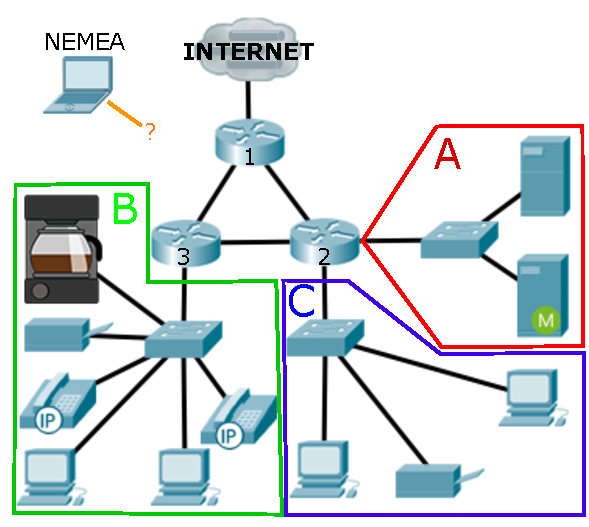
\includegraphics[scale=0.9]{Zapojeni.pdf}
        \caption[Příklad zapojení]{Příklad zapojení (vytvořeno v Cisco Packet Tracer a Inkscape)}
        \label{sit}
    \end{figure}
    
    \section{Zapojení systému NEMEA do sítě}
    NEMEA systém musíme umístit do sítě tak, aby bylo možné sledovat provoz. Tudíž jej musíme připojit k nějakému síťovému zařízení, které umožňuje funkcionalitu známou jako port-mirroring. Port-mirroring je funkce switche či routeru, která veškerý provoz na daném zařízení kopíruje na port, na němž je port-mirroring nastaven. Po nastavení switche či routeru a zapojení počítače, na kterém je systém NEMEA nainstalován, vidí systém veškerý provoz, který prochází daným síťovým zařízením, ale zatěžuje to CPU síťového zařízení. Ke stejnému účelu lze použít speciální zařízení TAP (Terminal Access Point), které umí kopírovat provoz.
    
    Rozhodnout, kam do sítě zapojit NEMEA systém s naším modulem, je složitější, než se zdá, jelikož každá volba ovlivní naměřený provoz. Na Obrázku \ref{sit} je vyobrazena síť, u které způsob zapojení NEMEA systému do sítě značně ovlivní získaná data. Pokud zapojíme modul do síťového přepínače (angl. switch) v segmentu \emph{A} s nastavení port-mirroring, získáme provoz mezi zařízeními v segmentu \emph{A}, provoz přístupů k zařízením  v segmentu \emph{A} ze segmentů \emph{B} a \emph{C} a provoz zařízení ze segmentu  \emph{A} do Internetu. Neodchytíme přitom komunikaci mezi segmenty \emph{B} a \emph{C} a taktéž komunikaci v rámci jejich segmentů. 
    
    Abychom získali i tuto komunikaci, mohli bychom nastavit na síťových zařízeních v jejich segmentech port-mirroring a kopii provozu z port-mirroring posílat tunelem mezi síťovými zařízení na náš modul v segmentu A. To by ale zatížilo klíčové linky mezi segmenty a navíc bychom měli některé záznamy duplicitní. Například záznam o komunikaci ze segmentu \emph{B} do segmentu \emph{C} by port-mirroring zachytil dvakrát, jednou v segmentu \emph{B} a podruhé v segmentu \emph{C}.
    
    Při zapojování našeho modulu do sítě musíme před volbou zvážit, jaký provoz nás zajímá nejvíce a co je cílem našeho měření. Již zmíněné zapojení do segmentu \emph{A} nám v příkladu získá seznam zařízení, které přistupují ke klíčovým serverům sítě.
    
    \section{Jednoznačné určení zařízení}
    Na segmentu lokální sítě jsme schopni bezpečně rozhodovat jaké IP adresy a v jakém čase je zařízení mělo. Díky viditelnosti MAC adres a DHCP protokolu může náš modul sledovat změny IP adres pro danou MAC adresu a tím spojit komunikaci jednoho zařízení pod více IP adresami.
    
    Na celé lokální síti to bohužel není možné, pokud neměříme ve všech segmentech, ale můžeme zachytávat DHCP komunikaci. Dané záznamy pak můžeme vypsat a tím pomoci správci sítě, aby měl přehled o komunikaci zařízeních s DHCP servery.
    
    
%===========================================================================================================
%===========================================================================================================
%===========================================================================================================
\chapter{NEMEA systém} \label{NEMEAsystem}
Network Measurements Analysis (NEMEA) \cite{NEMEA} je navržen s ohledem na stream-wise koncept, tzn. data jsou průběžně analyzována v paměti s minimálním ukládáním dat. Vyvíjen jako open-source projekt veřejně přístupný pro celosvětovou komunitu a navržen jak pro experimentální tak i provozní použití. Je schopen pracovat online, tzn. přímo připojen do sítě pracující s daty v jejím provozu, i offline, tzn. flow záznamy jsou uloženy a následně analyzovány nezávisle na provozu na síti. 

Systém NEMEA \cite{NEMEA} je navržen jako heterogenní modulární systém. Moduly jsou nezávislé procesy propojené jednosměrnými rozhraními pro komunikaci. Rozhraní přenášejí libovolná data ve formě toků zpráv --- flow záznamy, výsledky analýzy a další. Obrázek \ref{NEMEA_typical_flow} ukazuje jak probíhá typické monitorování provozu v systému NEMEA. 
\begin{figure}
    \centering
    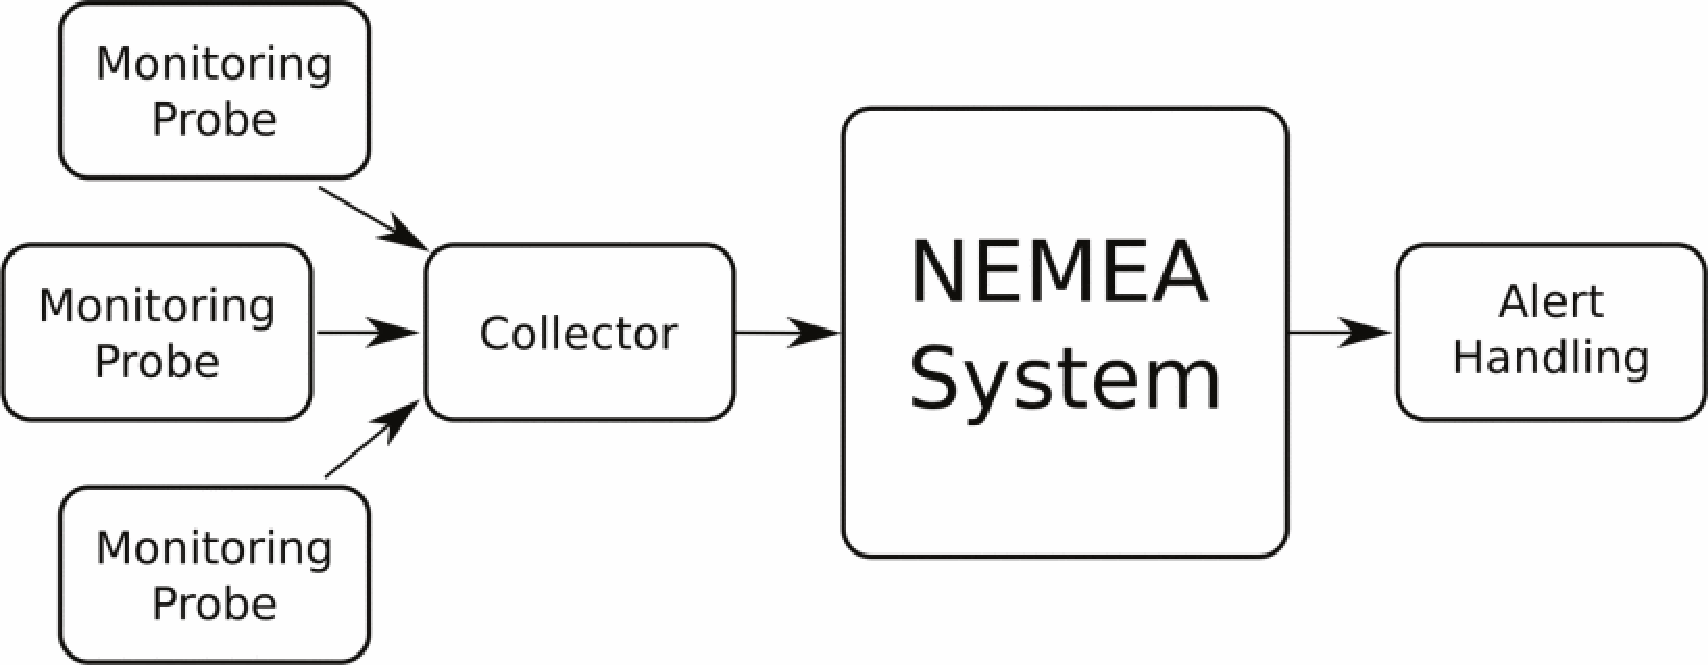
\includegraphics[width=\textwidth]{NEMEA1.pdf}
    \caption[Monitorování s NEMEA systémem]{Monitorování s NEMEA systémem \cite{NEMEA}}
    \label{NEMEA_typical_flow}
\end{figure}

\newpage
Infrastruktura monitorovacího systému je založena na exportu flow záznamů (pomocí monitorovacích sond), které jsou předávány k uložení (Collector) a analýze (NEMEA). Detekční moduly NEMEA vytvářejí výstrahy v jednotném formátu, který je vhodný pro následné zpracování a uložení.
    \section{Architektura}
    Jak již bylo řečeno, systém NEMEA \cite{NEMEA} je modulární systém složený z nezávislých modulů. Tyto moduly jsou kontrolovány a monitorovány pomocí nástroje nazvaného supervizor, který se vyplatí používat při větším počtu modulů a může běžet jako systémový daemon nebo v interaktivním režimu. Supervizor periodicky dostává od modulů stavové informace. Dále sleduje hardwarové zdroje modulů, jako například využití procesoru a pamětí RAM. Všechny moduly jsou stavěny na NEMEA Framework, tzn. moduly používají funkcionality, které jsou implementovány ve veřejných knihovnách NEMEA Frameworku. Každý modul obsahuje algoritmus, který zajišťuje jeho funkcionality, pro které byl navržen. Na Obrázku \ref{NEMEA_architecture} je architektura NEMEA systému vyobrazena. 
    \begin{figure}[h]
        \centering
        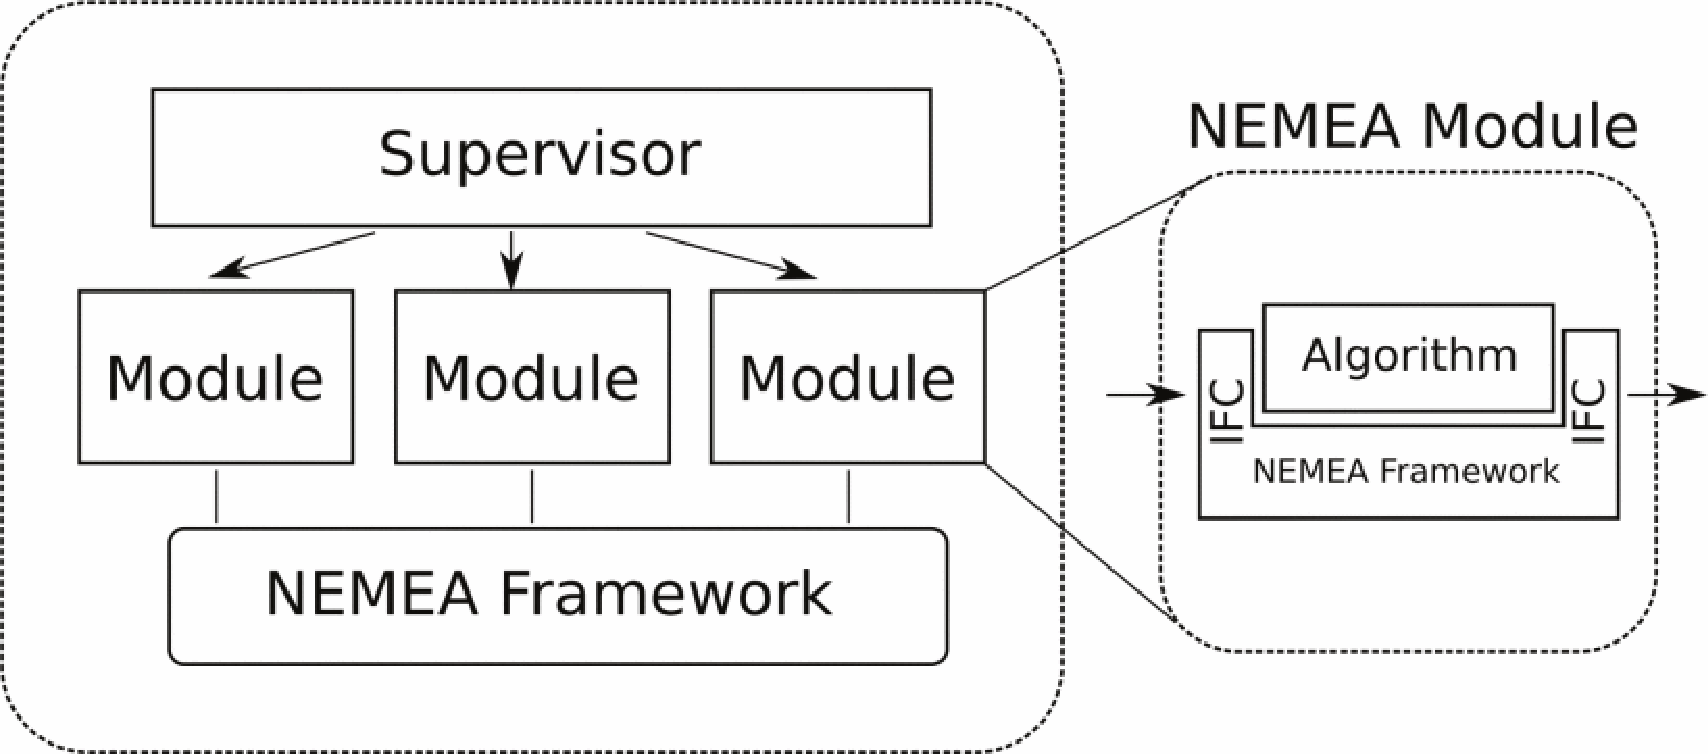
\includegraphics[width=\textwidth]{NEMEAArchitecture.pdf}
        \caption[Architektura NEMEA systému]{ Architektura NEMEA systému \cite{NEMEA}}
        \label{NEMEA_architecture}
    \end{figure}
    \newpage
    \section{Komunikační rozhraní}
    Moduly NEMEA systému spolu mohou komunikovat skrze TRAP Communication Interfaces (IFC). Přičemž každý IFC je vstup nebo výstup modulu a každý modul může mít libovolný počet vstupních a výstupních IFC. Data, které se posílají na IFC, jsou formátovaná do zpráv maximální velikosti 64 kB  a mohou obsahovat:
    \begin{itemize}
        \item flow záznam,
        \item výsledek algoritmu,
        \item statistické údaje nebo
        \item cokoliv jiného.
    \end{itemize}
    Existují různé druhy IFC a nejpodstatnější dva jsou založeny na UNIX soketech a TCP soketech. První se používá na komunikaci mezi jednotlivými moduly NEMEA systému a druhý se používá na komunikaci přes síť. Dále se může speciálními IFC zapisovat flow záznamy do souboru nebo při měření výkonu zapisovat data do blackhole.
    
    Přes IFC se mohou posílat data ve třech formátech a to:
    \begin{itemize}
        \item nestrukturovaná data,
        \item JSON formát nebo
        \item speciální binární formát UniRec systému NEMEA, ve kterém se přenášejí nejčastěji flow záznamy mezi moduly.
    \end{itemize}
    
    \section{Existující moduly důležité pro naši práci}
    
    \subsection{Flow meter}
    Tento modul ze síťového rozhraní či souboru vytvoří IP flows, které propaguje dalším modulům pomocí výstupního IFC. Pro nás modul to bude zdroj IP flows, které vytvoří z rámců přicházejících na síťové rozhraní většinou přes port-mirroring.
    
    \subsection{Logger}
    Tento modul může z IFC rozhraní, který naplňuje flow meter, získávat IP flows a ukládat je do souboru. Díky tomu může uživatel IP flows uložit do souboru a do našeho modulu tyto data poslat kdykoliv z uloženého souboru.
%===========================================================================================================
%===========================================================================================================
%===========================================================================================================
\chapter{Návrh}
    \section{PassiveAutodiscovery modul}
    Úkolem modulu je přiřadit zařízením štítky, zaznamenávat závislosti mezi zařízeními a následně je vykreslit do grafu závislostí.
    
    Aby modul mohl zařízení přiřadit štítek, musí porovnávat čísla portů, které dané zařízení používalo, se seznamem portů typických pro určitá zařízení, který vytvoříme. Tedy proces štítkování převedeme na vyhledávání, zda se použitý port nachází v seznamu.
    
    Co musíme řešit jako první je způsob uložení seznamu portů služeb, ukládání závislostí a dalších informací k zařízením. Ideálním řešením pro tento problém se nám nabízí databáze. Díky databázi můžeme nad daty provádět dotazy, kterými snadno přiřadíme zařízením štítky, rozhodneme o výrobci síťové karty či zmapování závislostí do grafu.
    
    \begin{figure}[h]
        \centering
        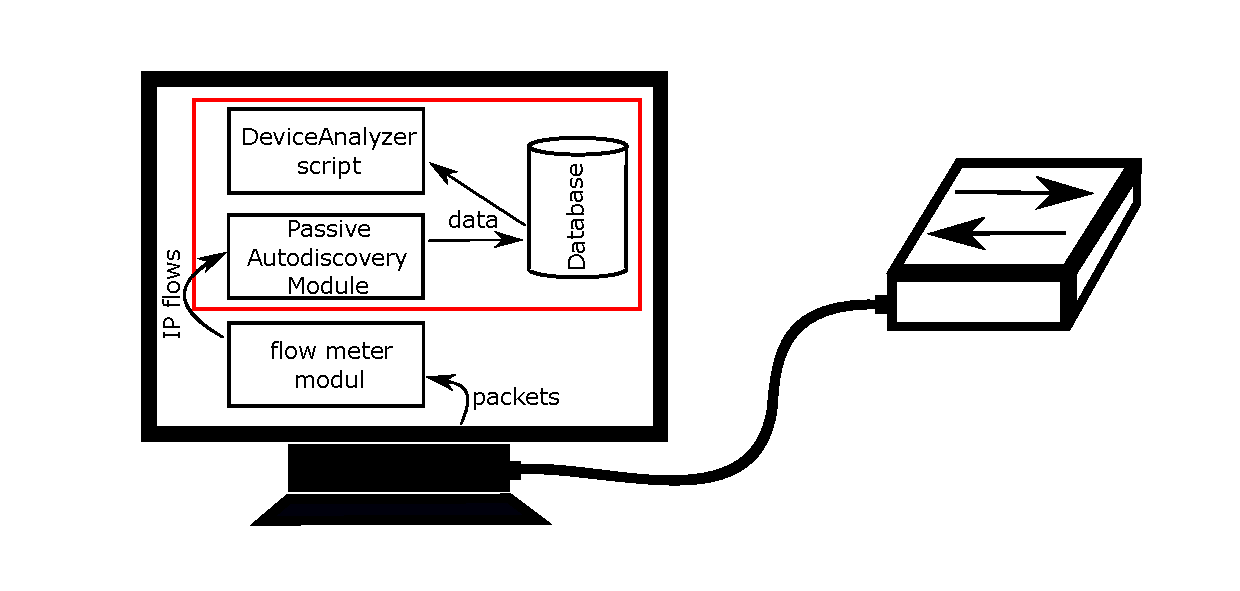
\includegraphics[width=\textwidth]{navrh.pdf}
        \caption[Návrh modulu]{Návrh modulu (vytvořeno v Inkscape)}
        \label{NavrhModulu}
    \end{figure}
    
    
    Jelikož můžeme předpokládat, že většina uživatelů našeho modulu bude chtít sledovat síť za účelem získání údajů o zařízeních v nějakém časovém okně, tak je pravděpodobné, že uživatel nejdříve spustí modul a na výsledky se bude chtít podívat až po skončení tohoto časového okna. Proto rozdělíme modul na dvě části.
    
    
    První část je PassiveAutodiscovery modul samotný, který spustíme spolu s flow meterem z NEMEA systému. Uživatel nejdříve nastaví náš modul a poté modul bude dle nastavení pracovat s IP flows. Ty mu v předpřipraveném stavu předloží flow meter. Modul poté z IP flows vytěží veškerá užitečná data jako je zdrojová a cílová IP adresa, zdrojová a cílová MAC adresa či zdrojový a cílový port. Tato data modul vhodně uloží do databáze tak, aby je předpřipravil druhé části modulu. Zároveň bude modul moci vypisovat nově nalezené informace, se kterými během ukládání pracuje.
    
    Druhá část programu bude skript, který bude pracovat s již uloženými daty v databázi a podá komplexní výstup o měření. To znamená, že projde v databázi všechna nalezená zařízení z měřených sítí a z databáze pomocí dotazů zjistí vše, co bylo z IP flows možné zjistit. Jeho primárním výstupem budou informace o zařízeních vypsané do příkazové řádky a obrázky grafů závislostí. Sekundárním bude JSON dokument obsahující všechny získané informace o zařízení. Tento skript nazveme DeviceAnalyzer a bude na našem modulu úplně nezávislý, takže bude moci být spuštěn kdykoliv po skončení běhu modulu a i během běhu modulu, ale pouze s voláním modulu.
    
    \begin{figure}
        \centering
        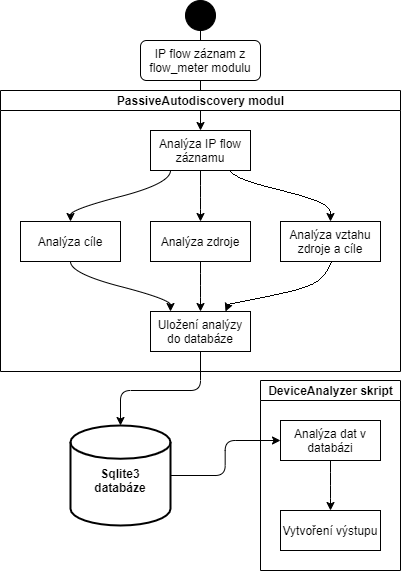
\includegraphics[width=\textwidth]{diagram.png}
        \caption[Diagram spolupráce částí modulu]{Diagram spolupráce částí modulu (vytvořeno v app.diagrams.net)}
        \label{Diagram}
    \end{figure}
    \newpage
    
    
    \section{Databáze}
        \subsection{Volba databáze}
        Při volbě databáze musíme zvážit, za jakým účelem budeme databázi používat. Náš modul pouze potřebuje nasbíraná data vhodně ukládat a poté na nich provádět SQL dotazy. Nepotřebujeme tudíž databázový server se spoustou konfiguračních a přístupových funkcí. Zároveň stavba databázového serveru může být problematická a jeho běh náročný na zdroje měřícího zařízení. Proto hledáme databázi, která neběží na serveru, ale rychle a snadno se pomocí jednoduchých skriptů vytvoří, spustí a dokáže provádět dotazy.
        
        Proto jsme zvolili SQLite3 databázi, která pracuje pouze se souborem, nad kterým provádí dotazy. Bohužel při každém vkládání dat do souboru SQLite3 čeká, až se do souboru, který představuje databázi, zapíší data, což je pomalejší než běžné databáze. Tuto nevýhodu se pokusíme co nejvíce minimalizovat možností používat RAM paměť pro průběžné ukládání databáze.
        
        \subsection{Databázový model}
        Nejdříve navrhneme podobu tabulek pro přiřazování štítků, což je primární funkcionalita našeho modulu. Jako základní kámen pro celou naší databázi musí být tabulka obsahující všechna nalezená lokální zařízení. Tuto tabulku pojmenujeme \emph{LocalDevice}. 
        
        K přiřazování štítků potřebujeme tabulku obsahující základní informace o dobře známých a registrovaných portech, jejichž rozložení máme vyobrazeno v Tabulce \ref{Ports}. Tudíž vytvoříme tabulku \emph{Ports}, do které tyto informace vložíme z oficiálního zdroje \cite{IANA}. 
        Dále vytvoříme tabulku pro porty používané specifickými zařízeními. Nazveme jí \emph{Services} a vložíme do ní námi vytvořený seznam pro štítkování obsahující ke každému portu typ zařízení a popis použití portu u daného zařízení. 
        
        Tabulky \emph{Services} a \emph{LocalDevice} spojíme pomocí tabulky \emph{LocalServices}, do které budeme přidávat k jednotlivým zařízením použité porty. Z této tabulky pak snadno přes dotazy získáme štítky pro jednotlivá zařízení. Tato část návrhu databáze je vykreslena na Obrázku \ref{DBLabels}.
        \begin{figure}[h]
            \centering
            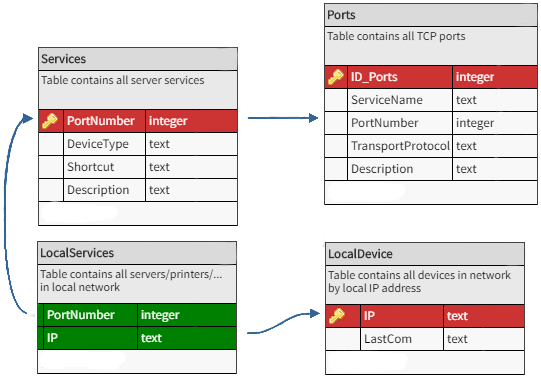
\includegraphics[width=\textwidth]{databaze_services.png}
            \caption[Přiřazování štítků]{Přiřazování štítků (vytvořeno v \url{https://app.dbdesigner.net/}, upraveno v Adobe Photoshop) }
            \label{DBLabels}
        \end{figure}
        
        Další důležitou funkcionalitou našeho modulu je vyhledávání závislostí mezi zařízeními.
        
        K základní tabulce lokálních zařízení \emph{LocalDevice} přidáme tabulku se závislostmi mezi lokálními zařízeními, kterou pojmenujeme \emph{Dependencies}. Tabulka nám umožní vkládat jedinečné závislosti. Za jedinečnou závislost považujeme takovou závislost, u které je vazba mezi dvěma lokálními zařízeními a port použitý jedním ze zařízení se nachází v tabulce \emph{Services}, respektive \emph{Ports}. Pokud se port nalezne v tabulce \emph{Services} je přidán štítek danému zařízení v tabulce \emph{LocalServices}. Takže jedinečná závislost je vazba zařízení A na zařízení B, přičemž port zařízení B, respektive port zařízení A, je známý či registrovaný port.
        
        
        Dále vytvoříme tabulku pro přístupy lokálních zařízení do internetu (s IP adresou z globálního prefixu). Tabulka bude téměř shodná s tabulkou \emph{Dependencies}, ale jedná se o vazbu lokálního zařízení na zařízení v internetu. Tuto tabulku nazveme \emph{Global}. K zařízením z globální sítě taktéž vytvoříme tabulku typů zařízení \emph{GlobalServices}. Nákres na Obrázku \ref{DBDependencies}.
        \begin{figure}[h]
            \centering
            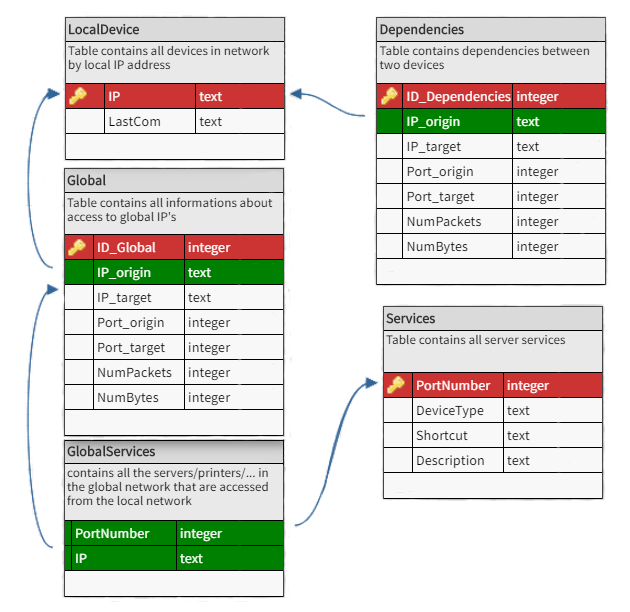
\includegraphics[width=\textwidth]{databaze_zavislosti.png}
            \caption[Závislosti mezi zařízeními]{Závislosti mezi zařízeními (vytvořeno v \url{https://app.dbdesigner.net/}, upraveno v Adobe Photoshop) }
            \label{DBDependencies}
        \end{figure}
        
        Další tabulky, které budeme potřebovat, jsou \emph{MAC}, \emph{VendorsMAC}, \emph{DHCP} a \emph{Routers} zobrazené na Obrázku \ref{DBMAC}. Tabulka \emph{MAC} slouží k uložení MAC adresy k IP adresám na lokálním segmentu sítě. Úzce spolupracuje s tabulkou \emph{Routers}, do které jsou v případě zjištění, že MAC adresa patří routeru, přelijí záznamy dané MAC adresy, které se nacházejí v tabulce \emph{MAC}. V tabulce \emph{Routers} se poté nachází MAC adresy routerů a všechny IP adresy, které jsou za těmito routery a komunikovali do segmentu sítě, ve kterém měříme.
        
        Tabulka \emph{DHCP} slouží k ukládání DHCP záznamů k jednotlivým zařízením, podle čehož poté rozhodujeme o tom, zda je MAC adresa routerem či nikoliv. Poslední přidaná tabulka obsahuje informace o výrobcích síťových karet, rozpoznatelných podle první poloviny MAC adresy.
        
        \begin{figure}[h]
            \centering
            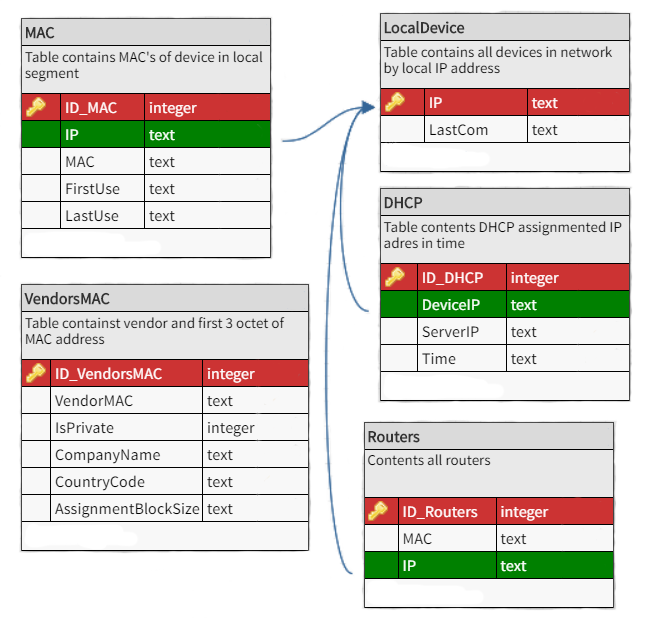
\includegraphics[width=\textwidth]{databaze_MAC.png}
            \caption[MAC a DHCP]{MAC a DHCP (vytvořeno v \url{https://app.dbdesigner.net/}, upraveno v Adobe Photoshop) }
            \label{DBMAC}
        \end{figure}
        
        \newpage
        
        Na Obrázku \ref{DBTime} můžeme vidět návrh dvou tabulek \emph{DependenciesTime} a \emph{GlobalTime}, které slouží pro uložení časových záznamů závislostí. Pro každý IP flow záznam uchováváme o jakou závislost se jedná, čas a počet paketů v daném IP flow. Ze záznamů pak můžeme snadno zrekonstruovat jak probíhala komunikace pro každou závislost.
        
        \begin{figure}[h]
            \centering
            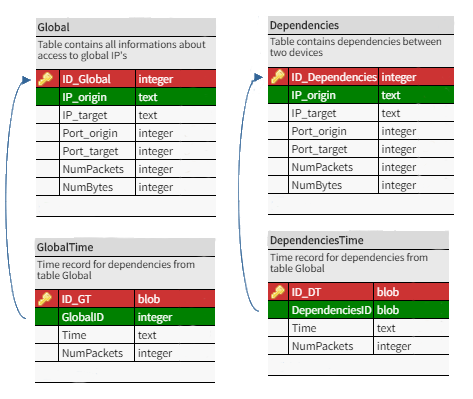
\includegraphics[width=\textwidth]{TimeTables.png}
            \caption[Časové záznamy]{Časové záznamy (vytvořeno v \url{https://app.dbdesigner.net/}, upraveno v Adobe Photoshop) }
            \label{DBTime}
        \end{figure}
        
        \newpage
        
        Poslední potřebnou tabulkou je \emph{Filter}, kterou vytvoříme pro filtrování neúplného provozu. Tabulka obsahuje minimální počet paketů pro úplný provoz pro specifický protokol s daným číslem portu. Návrh můžeme vidět na Obrázku \ref{DBFilter}
        \begin{figure}[h]
            \centering
            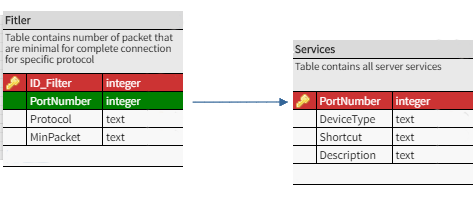
\includegraphics[width=\textwidth]{Filter_Services.png}
            \caption[Filtrování komunikace]{Filtrování komunikace (vytvořeno v \url{https://app.dbdesigner.net/}, upraveno v Adobe Photoshop) }
            \label{DBFilter}
        \end{figure}
        
        \subsection{Vytvoření databáze}
        Aby uživatel nemusel databázi vytvářet manuálně, tak je součástí výstupu této práce instalační skript, který automaticky databázi vytvoří z SQL souboru a vloží data do tabulek \emph{Services}, \emph{Filter}, \emph{Ports} a \emph{VendorsMAC}.


%high-level pohled, architektura řešení, související “sousedící” komponenty/systémy, z high-level pohledu popsat co bylo řešeno v této práci, datový model, pokud je potřeba
%===========================================================================================================
%===========================================================================================================
%===========================================================================================================
\chapter{Implementace}
%vysvětlení použitého algoritmu, vysvětlení funkcionality a její použití, low-level pohled jen na to hlavní / zajímavé /důležité
V této kapitole vysvětlíme fungování naší implementace jednotlivých částí naší práce a ukážeme si nejdůležitější prvky implementace. Veškeré části práce jsou programované v jazyce python verze 3.6.
    \section{CreateScript}
    Python skript \uv{CreateScript.py} nejdříve zjistí, zda databáze se jménem zadaným v parametru -d již existuje, pokud ano, zeptá se nás, jestli jí chceme přemazat či nikoliv. To nám dává možnost zálohovat si databázi.
    Poté skript vytvoří ze souboru \uv{Database\_sqlite\_create.sql} databázi. 
    
    Jakmile je databáze vytvořená přistoupí skript pomocí knihovny \emph{urllib} \cite{URLLIB} na url odkazy, ze kterých stáhne data pro tabulky \emph{Ports} a \emph{VendorsMAC}. Pokud se mu nepodaří nějakou tabulku naplnit daty z internetu, použije naší zálohu, která je součástí vyvinutého programu. Nakonec skript použije námi vytvoření seznam zařízení a jejich často používaných portů k naplnění tabulky \emph{Services}.
    
    \section{PassiveAutodiscovery modul}
    Náš výchozí modul primárně naslouchá na IFC rozhraní popsané v kapitole NEMEA systém a získané IP flows distribuuje do skriptu \uv{Collector.py}, který IP flows zařazuje do databáze. Pro tuto funkcionalitu využívá především knihovny \emph{pytrap} \cite{NEMEA} z NEMEA systému.
    
    Dále nám tento modul slouží jako komunikační rozhraní. Při spuštění pomocí parametrů určíme nastavení, kterým zpřesníme měření i následnou analýzu a při jeho běhu zde můžeme při vhodném nastavení nalézt základní informační výpisy o nově nalezených zařízeních či závislostí.
    
    \section{Collector}
    Skript Collector obsahuje obsahuje důležitou stejnojmennou funkci, kterou volá \uv{PassiveAutodiscovery.py} modul. Funkce dále dle nastavení zadané v modulu vyplňuje databázi \uv{Database.db} voláním dalších pomocných funkcí. Přičemž jejich volání záleží na IP adresách komunikujících zařízeních. 
    
    Pokud jsou obě zařízení lokální tak se pro ně volají funkce na přidání lokálního zařízení do tabulky \emph{LocalDevice}, funkce pro kontrolování, zda zařízení nekomunikují pomocí specifického portu pro nějaké zařízení a nakonec funkce pro závislost dvou lokálních zařízení. Pokud je jedno z nich modulem považováno za lokální (zařízení z privátního rozsahu IP adres či z explicitně zadané sítě) a druhé nikoliv, tak se funkce volají pro jedno z nich a zároveň se volá funkce pro globální závislosti. V případě, že ani jedno zařízení není lokální, funkce skončí bez žádných akcí.

    \uv{Collector.py} považuje při analýze za lokální zařízení zařazované do tabulky \emph{LocalDevice} buď zařízení s IP adresou z privátních rozsahů, nebo z rozsahů námi zadaných při spuštění modulu. Každé nové zařízení je poté přiřazeno do tabulky, a pokud v ní již existuje, tak se aktualizuje čas poslední aktivity.
    
    Ke každému lokálnímu zařízení se zaznamenávají jednotlivé štítky, které se snadno naleznou jednoduchým SQL dotazem:
    
    \begin{verbatim}
        SELECT * FROM Services WHERE PortNumber = {port};\end{verbatim}
     kde port je použitý port na transportní vrstvě TCP/IP modelu zařízením v daném IP flow.
    
    Pokud dotaz nalezne záznam, tak má zařízení roli zapsanou ve vybraném řádku z tabulky \emph{Services}. Samozřejmě musíme před vložením záznamu do tabulky \emph{LocalServices} zjistit, zda se totožný záznam již v tabulce nenachází, abychom nevytvářeli duplicitní záznamy.
    

    Závislosti jak lokální, tak globální, se přidávají, pokud alespoň jeden z použitých portů v daném IP flow existuje v tabulce \emph{Ports}, čili zda je port registrovaný či dobře známý. Pokud stejný záznam již existuje, tak skript navýší počet přenesených paketů v dané závislosti.
    
    \section{DeviceAnalyzer}
    Skript \uv{DeviceAnalyzer.py} vytváří hlavní výstup celého modulu a pracuje zcela nezávisle na \uv{PassiveAutodiscovery.py}. To znamená, že jej uživatel může spustit kdykoliv, pokud existuje databáze \uv{Database.db} a jsou v ní nasbíraná nějaká data a zároveň žádný jiný skript do ní zrovna nezapisuje. Aby bylo možné pustit jej během měření sítě pomocí \uv{Passiveautodiscovery.py}, musíme toto měření pozastavit.
    
    \newpage
    Pomocí tohoto skriptu se nám zobrazí buď analýza pro jedno konkrétní zadané zařízení nebo kompletní analýza pro každé zařízení obsahující:
    \begin{itemize}
        \item \emph{IP adresu}, ke které je přiřazená komunikace na lokální a globální sítí dále analyzovaná
        \item \emph{další IP adresy} pokud se podařilo zjistit, že jedno zařízení komunikuje v síti pod více IP adresami (IPv4, IPv6 a změny na těchto adresách)
        \item \emph{MAC adresu} pokud je zařízení ve stejném segmentu sítě jako měřící zařízení
        \item \emph{Výrobce síťové karty} pokud máme k dispozici MAC adresu
        \item \emph{Přiřazené štítky} spolu s popiskem obsahující jaký protokol byl použit
        \item \emph{záznamy DHCP}
        \item \emph{Lokální závislosti} mezi zařízeními, které \uv{Collector} považoval v době měření za lokální
        \item \emph{Statistiku pro lokální závislosti} uvádějící v procentech, jaké protokoly byly nejpoužívanější
        \item \emph{Globální závislosti} obsahujícím přístupy zařízení mimo síť
        \item \emph{Statistiku pro globální závislosti} uvádějící v procentech, jaké protokoly byly nejpoužívanější
    \end{itemize}
    Tyto informace se ve většině případů získávají z databáze vhodnými SQL dotazy. V konkrétním případě si můžeme ukázat, jak vypadá vyhledání přiřazených štítků pro výpis:
    \begin{verbatim}
    SELECT S.PortNumber, S.DeviceType, S.Shortcut, S.Description 
    FROM LocalServices LS JOIN Services S 
    ON LS.PortNumber=S.PortNumber WHERE LS.IP='{ip}';\end{verbatim}
     kde ip je IP adresa lokálního zařízení, pro které vypisujeme přiřazené štítky. Tento dotaz nám vrátí všechny štítky, které byly přiřazeny danému zařízení.
    
    Nakonec analýzy zařízení se vypíše statistika celé sítě uvádějící v procentech, jaká zařízení z lokální sítě používala síť v době měření nejvíce. Pro přehledný výpis statistiky se používá knihovna \emph{termgraph} \cite{TERMGRAPH}. Pokud uživatel zvolí, tak se vytvoří grafy závislostí, které jsou uloženy do souborů. Grafy se vytváří z tabulek \emph{Dependencies} a \emph{Global} pomocí knihoven \emph{networkx} \cite{NETWORKX} a \emph{matplotlib} \cite{MATPLOTLIB}. 
    
    Přičemž závislosti lokálních zařízení z tabulky \emph{Dependencies} jsou rozděleny na dva grafy. Jeden pro IPv4 a druhý pro IPv6 verze IP adres. Tyto dvě verze spolu nikdy nekomunikují, proto graf závislostí s oběma verzemi IP adres byl rozdělen na dva podgrafy, které se knihovna \emph{matplotlib} \cite{MATPLOTLIB} snažila oddělit, čímž způsobila zmenšení obou podgrafů a ty se staly nepřehledné. Kvůli tomu jsme se rozhodli rozdělit graf na verze. Grafy globálních závislostí jsou vytvářeny vždy pro každé zařízení zvlášť, čímž vzniknou grafy typu hvězda. Skript nastavíme pomocí přepínačů při spouštění. Také nám umožňuje vytvořit bipartitní graf, ve kterém se v jedná partitě nacházejí lokální zařízení a ve druhé partitě globální zařízení, přičemž globální zařízení se v grafu nacházejí pouze pokud k nim přistupovalo více lokálních zařízení.
    
    Dalšími důležitými knihovnami jsou \emph{ipaddress} \cite{IPADDRESS} a \emph{sqlite3} \cite{SQLITE3}. První používáme pro práci s IP adresami a druhou pro připojení a následnou komunikaci s databází.

    
%===========================================================================================================
%===========================================================================================================
%===========================================================================================================
\chapter{Testování}
%DŮLEŽITÁ KAPITOLA popis testování (odůvodnění, že to tak stačilo otestovat), má ukázat že to funguje a taky jak dobře to funguje, porovnání s existujícím řešením pokud je, prezentace výsledků, vyhodnocení závislosti na různých vstupech pokud se nějak liší, propustnost, výsledky z nasazení
V této kapitole si ukážeme ukázky výstupu vyvinutých nástrojů, které byly nasazeny v sítích pro pilotní testování. Také si předvedeme časové a paměťové náročnosti vyvinutých nástrojů.
    \section{Domácí síť}
    Nejdříve provedeme testování na malé lokální síti, která se často nachází ve většině domácností. Provedeme měření způsobem přímého zapojení do sítě, jejíž zapojení jsme v upravené podobě vykreslili do Obrázku \ref{HomeNetwork} (většina DSL modemů neumí port-mirroring, proto jsme pro měření umístili do sítě switch, který tuto funkcionalitu umožňuje).
    
    
    \begin{figure}[h]
        \centering
        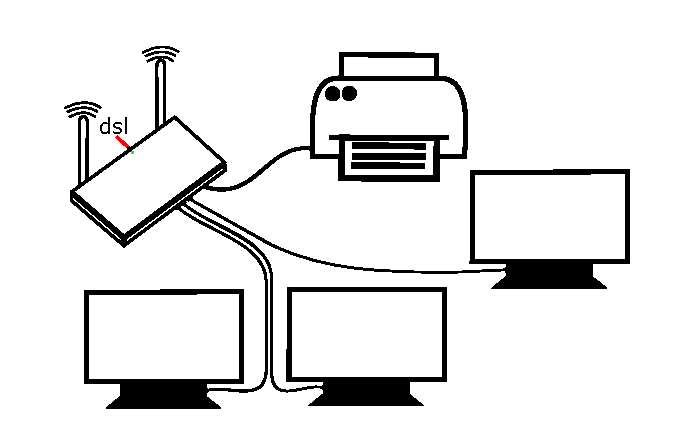
\includegraphics[scale=0.9]{HomeNetwork.pdf}
        \caption[Nákres domácí sítě]{Nákres domácí sítě (vytvořeno Inkscape) }
        \label{HomeNetwork}
    \end{figure}
    
    Cílem měření na této konkrétní síti je odhalit z komunikace, zda je v síti tiskárna a počítače. Spustíme náš modul a počkáme, než se nám nasbírají potřebná data. Poté spustíme skript \emph{DeviceAnalyzer} a výsledek vypíšeme do příkazové řádky. 
    
    Měření jsme prováděli jen po dobu, než jsme si byli jistí, že proběhla potřebná komunikace k rozpoznání důležitých zařízení. Na Obrázku \ref{PCHome} můžeme vidět výstup \emph{DeviceAnalyzer} skriptu pro jeden z počítačů, přičemž globální závislosti byly nezajímavé, a proto jsme je z výstupu smazali. Všimněme si, že náš modul správně určil operační systém počítače a taktéž, dle přístupů na webové a e-mailové služby, rozhodl o tom, že se jedná o koncové zařízení. 
    
    \begin{figure}[h!]
        \centering
        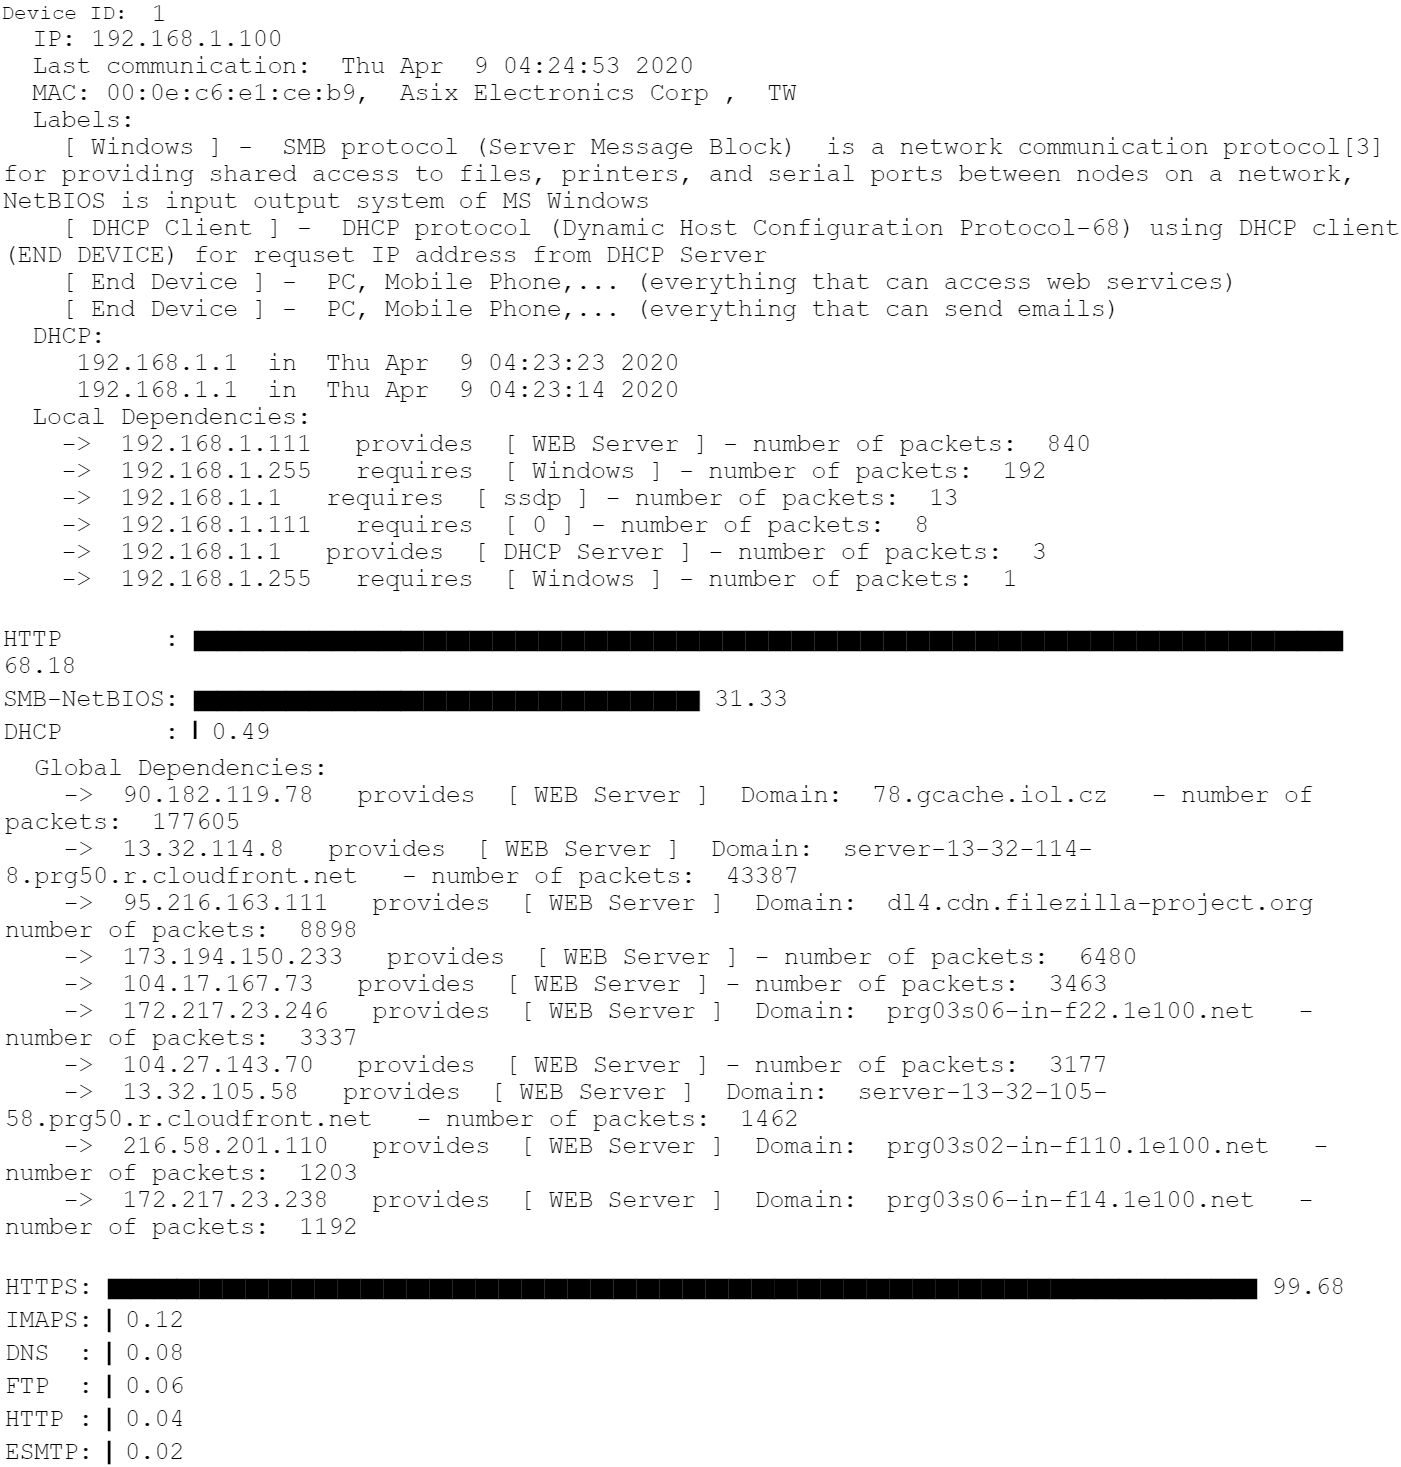
\includegraphics[scale=0.36]{PC_HomeNetwork.png}
        \caption[Ukázka měření: Počítač v domácí síti]{Počítač}
        \label{PCHome}
    \end{figure}
    \newpage
    
    Dále si povšimněme, že počítač získával IP adresu od serveru pomocí DHCP, proto má zařízení přiřazen štítek \emph{DHCP Client}. V DHCP záznamech můžeme vidět kdy a od jakého serveru získával IP adresu. V lokálních zařízeních vidíme závislost k \emph{192.168.1.111}, který podle modulu provozoval \emph{WEB Server}. Víme, že přes protokol HTTP se nepřenáší jen webové služby, takže můžeme vytušit, že se nejedná o skutečný webový server. V našem případě víme, že zařízení je switch a pomocí protokolu HTTP se v době měření přistupovalo k nastavení switche přes webové rozhraní.
    
    Na dalším Obrázku \ref{RouterHome} je vyobrazen výstup pro další zařízení, tentokrát se jedná o router, který zároveň lokální síti poskytoval DHCP a DNS služby. Podstatnou informací jsou IP adresy, pod kterými zařízení v síti vystupovalo. 
    
    Posledním zajímavým zařízením v této síti je tiskárna. Výstup pro ni můžeme vidět na Obrázku \ref{PrinterHome}. Můžeme si všimnout, že na tiskárně v době měření tisklo pouze jedno zařízení a použilo k domu dva protokoly a to PDP a IPP. 
    %\clearpage
    \begin{figure}[h!]
        \centering
        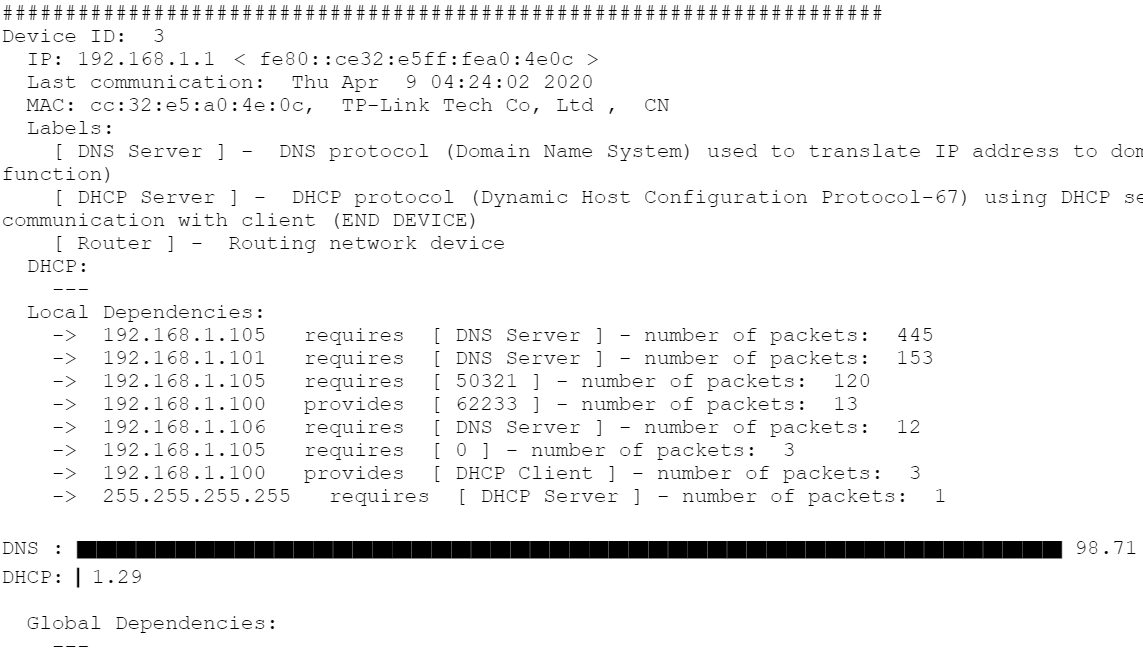
\includegraphics[width=\textwidth]{Router_HomeNetwork.png}
        \caption[Ukázka měření: Router v domácí síti]{Router}
        \label{RouterHome}
    \end{figure}
    \begin{figure}[h!]
        \centering
        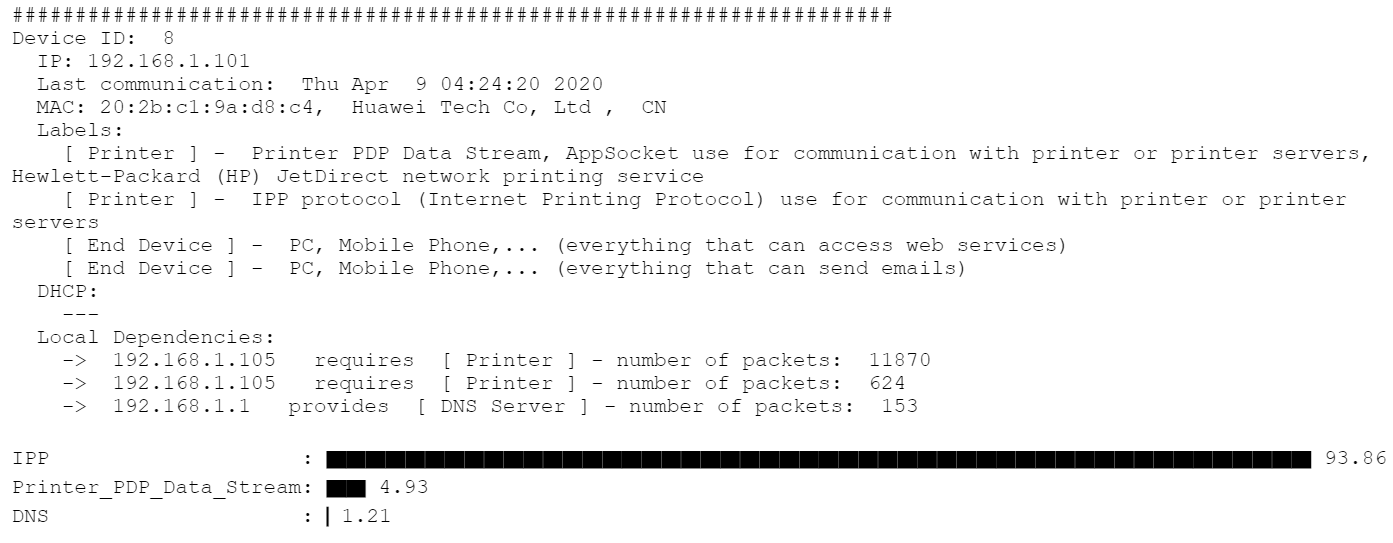
\includegraphics[width=\textwidth]{Printer_HomeNetwork.png}
        \caption[Ukázka měření: Tiskárna v domácí síti]{Tiskárna}
        \label{PrinterHome}
    \end{figure}
    
    Na Obrázku \ref{GrafHome} můžeme vidět graf závislostí na lokální síti, který modul vytvořil na základě pozorované komunikace.
    \begin{figure}[h!]
        \centering
        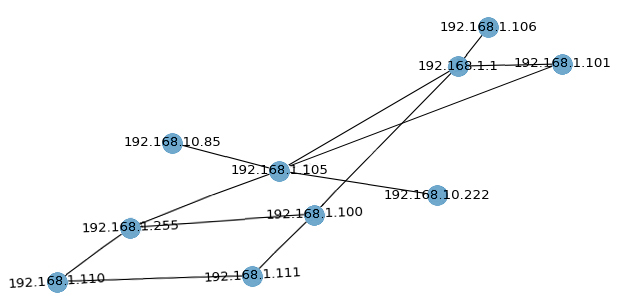
\includegraphics[width=\textwidth]{Graph_Local_IPv4_HomeNetwork.jpg}
        \caption[Ukázka měření: Graf lokálních závislostí v domácí síti]{Graf lokálních závislostí pro IPv4 adresy}
        \label{GrafHome}
    \end{figure}
    
    \clearpage
    \newpage
    \section{Síť v kanceláři}
    Sítě v kancelářích většinou obsahují pracovní počítače, tiskárny a zařízení pro sdílení souborů, jak souborové servery, tak sdílené disky. Ze serverů se objevují DHCP a DNS servery, které podporují činnosti počítačů. Ve větších firemních sítích se samozřejmě objevují nejrůznější autentizační, souborové, webové či e-mailové servery, ke kterým přistupují jak zařízení z lokální sítě, tak zařízení z internetu. 
    
    Pro toto testování jsme naměřili síť laboratoře monitorování síťového provozu na Fakultě Informačních Technologií ČVUT a vytvořili záznam v souboru \emph{.trapcap}, ale v záznamu nemáme informace o MAC adresách. Nyní si ukážeme výstup o vybraných zajímavých zařízeních.

    Na Obrázku \ref{Mobil} vidíme výstup o zařízení, které přistupuje na webové služby, přijímá IP adresu prostřednictvím DHCP protokolu a zároveň používá protokol typický pro volání přes internet pro mobilní zařízení. Z toho snadno odhadneme, že zařízení je pravděpodobně chytrý mobilní telefon připojený k Wi-Fi.
    
    \begin{figure}[h!]
        \centering
        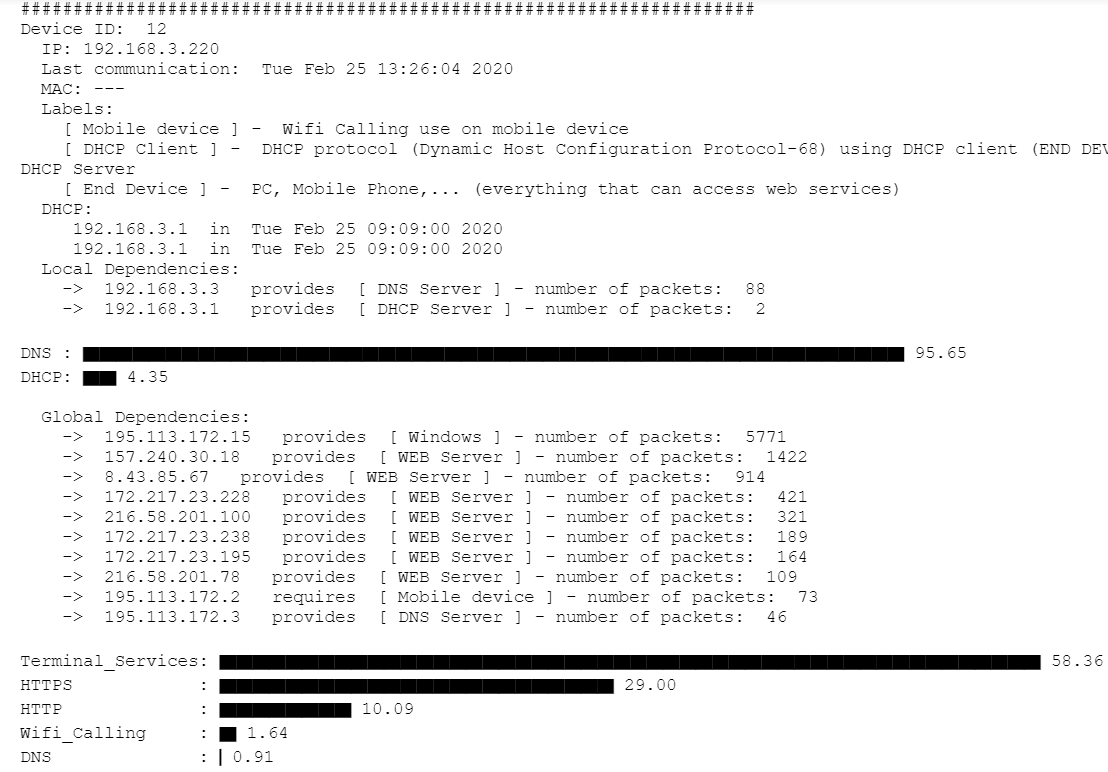
\includegraphics[width=\textwidth]{FITKancl_MObile.png}
        \caption[Ukázka měření: Mobilní zařízení v kancelářské síti]{Mobilní zařízení}
        \label{Mobil}
    \end{figure}
    
    
    Mobilní telefon v lokální síti komunikuje se dvěma různými zařízeními, a to s DHCP Serverem s IP adresou končící na \emph{.1}, který mu přidělil IP adresu a DNS Serverem s IP adresou končící na \emph{.3}, který DNS dotazy dále distribuuje do internetu. Při pohledu na výpisy těchto dvou zařízení zjistíme, že zařízení \emph{.1} zároveň poskytuje DNS službu a to právě pro zařízení \emph{.3}, které je DNS Serverem pro většinu zařízení v síti, proto je pravděpodobné, že zařízení \emph{.1} je routerem. Nicméně bez MAC adres náš modul nemohl rozhodnout, že je toto zařízení routerem i když tomu tak pravděpodobně je. Na Obrázku \ref{DNSServer} můžeme vidět výstup zařízení \emph{.3}, tedy DNS Serveru. Z něj si snadno všimneme, že hlavní globální závislost je s IP adresou \emph{1.1.1.1}, která je známá poskytováním DNS služeb.
    
    \begin{figure}[h!]
        \centering
        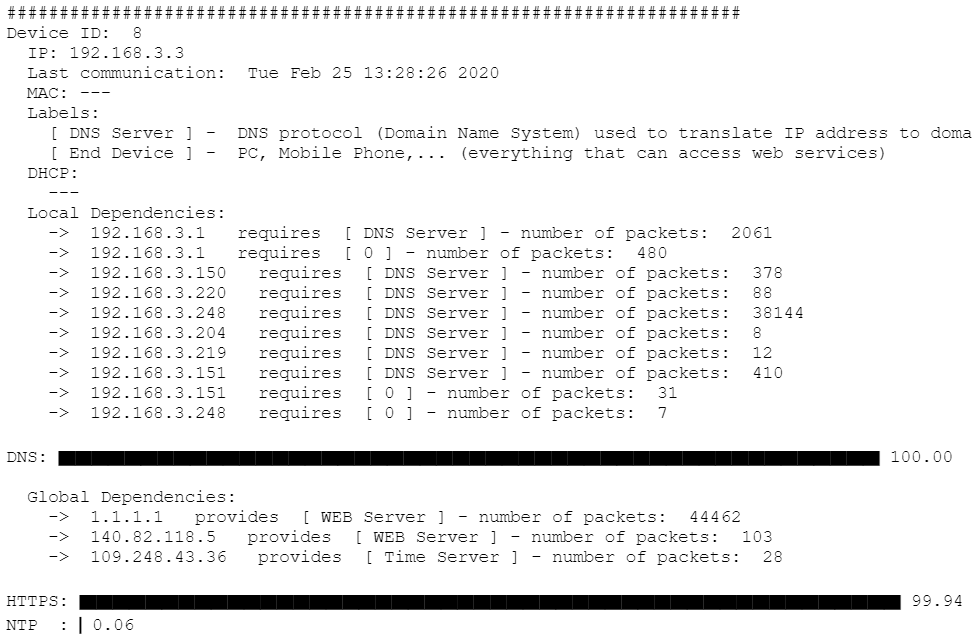
\includegraphics[width=\textwidth]{DNSServer.png}
        \caption[Ukázka měření: DNS Server v kancelářské síti]{DNS Server}
        \label{DNSServer}
    \end{figure}
    
    Na Obrázku \ref{Statistic} je vykresleno používání sítě zařízeními v procentech, ze kterého přehledně vidíme, jaká zařízení v síti přenesli nejvíce paketům. Síť nejvíce používaly osobní počítače.
    
    \begin{figure}[h!]
        \centering
        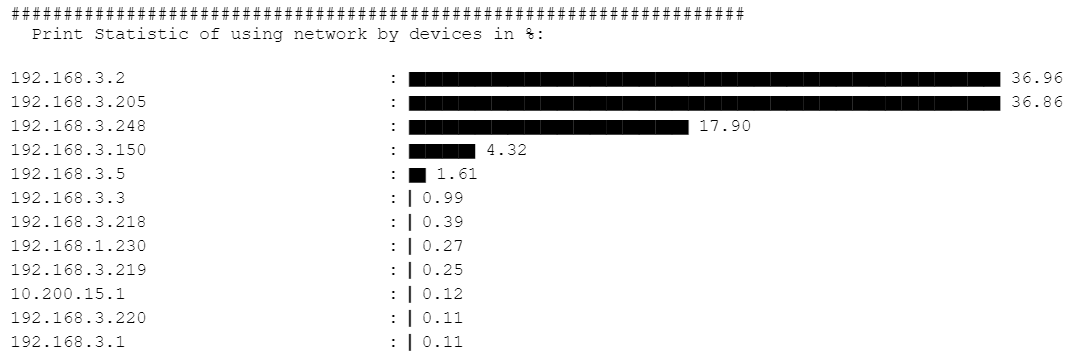
\includegraphics[width=\textwidth]{statistic.png}
        \caption[Ukázka měření: Statistika pro síť v kanceláři]{Statistika používání sítě}
        \label{Statistic}
    \end{figure}
    
    
    Na Obrázku \ref{GrafIPv4} je vykreslen graf závislostí pro zařízení s IP adresou verze 4. Z něj vidíme, že nejvytíženější zařízení v síti je zařízení s IP adresou končící na \emph{.1}, jejž jsme ručně označili za router a zařízení s IP adresou končící na \emph{.3}, které je DNS Serverem. 
    
    \begin{figure}[h!]
        \centering
        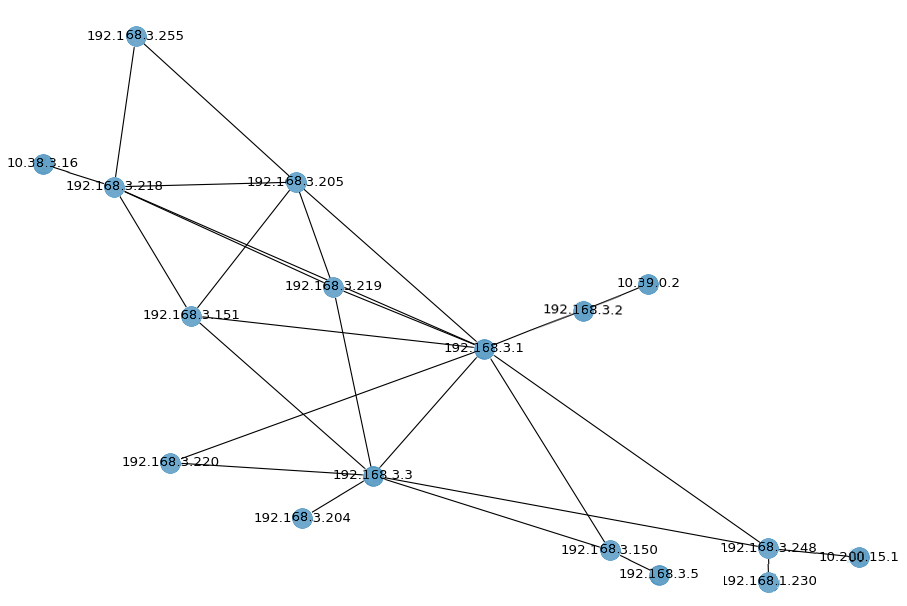
\includegraphics[width=\textwidth]{FITKancl_IPv4.jpg}
        \caption[Ukázka měření: Graf lokálních závislostí IPv4 pro síť v kanceláři]{Graf lokálních závislostí IPv4}
        \label{GrafIPv4}
    \end{figure}
    Na Obrázku \ref{GrafBipartite} je vykreslen graf závislostí mezi lokálními (těmi zařízeními, které modul považuje za lokální) a globálními zařízeními. Přičemž globální zařízení se do grafu dostanou pouze tehdy pokud k nim přistoupí více lokálních zařízení. Tím vznikne bipartitní graf, kde na levé straně jsou lokální zařízení a na pravé straně jsou globální zařízení.
    
    Dále můžeme při měření použít parametr \emph{-T}, kterým zapneme práci s časem u závislostí, takže modul vyplní tabulky \emph{DependenciesTime} a \emph{GlobalTime} časovými údaji o závislostech z tabulek \emph{Dependencies} a \emph{Global}. Výstup z analýzy \emph{DeviceAnalyzer} skriptu je poté vyobrazen na Obrázku \ref{GrafTime}, na kterém můžeme vidět přenesené pakety v závislosti na čase.
    
    Stejný typ grafu, který ukazuje aktivitu zařízení v době měření, můžeme vytvořit pomocí parametru \emph{-A}.
    \newpage
    
    \begin{figure}[h!]
        \centering
        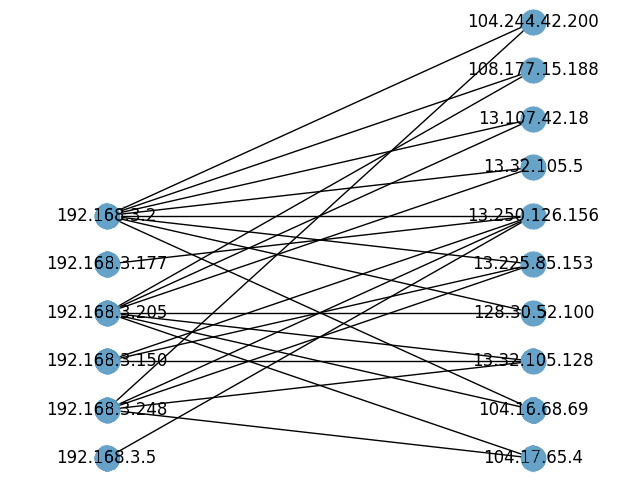
\includegraphics[scale=0.7]{Biparite_graph}
        \caption[Ukázka měření: Bipartitní graf závislostí mezi lokálními a globálními zařízeními pro síť v kanceláři]{Bipartitní graf závislostí mezi lokálními a globálními zařízeními}
        \label{GrafBipartite}
    \end{figure}
    
    \begin{figure}[h!]
        \centering
        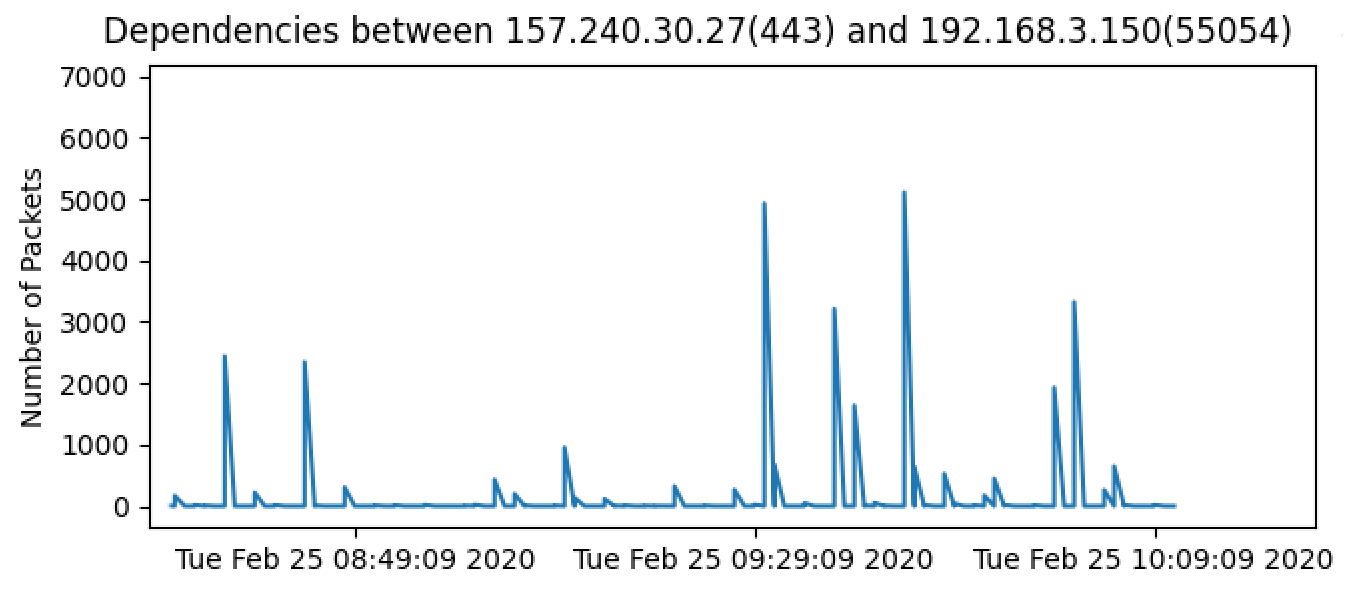
\includegraphics[width=\textwidth]{TimeGraph.png}
        \caption[Ukázka měření: Graf používání závislosti v čase pro síť v kanceláři]{Graf používání závislosti v čase}
        \label{GrafTime}
    \end{figure}
    
    \newpage
    \section{Globální síť}
    Nakonec pro testování zkusme náš modul vhodně nastavit tak, aby co nejlépe fungoval na globální síti. Pro tento účel jsme ve spolupráci se sdružením CESNET, operátorem národní akademické infrastruktury, získali anonymizované záznamy komunikace rozdělené po hodinách z globálních rozsahů ČVUT (\emph{147.32.232.0/24}), VUT (\emph{147.229.13.0/24}) a CESNET (\emph{195.113.172.0/24}). Veřejné IP adresy byly ve výstupu zanonymizovány.
    
    Jelikož je náš modul primárně určen na práci na lokálních sítích, tak musíme modulu nastavit IP adresy sítí, které chceme sledovat. Modul proto spustíme takto:
    \shellcmd{./PassiveAutodiscovery.py -i f:GlobalRecord.trapcap -d Database \\ -N 147.32.232.0/24  147.229.13.0/24 195.113.172.0/24 -! -G -U }
     kde v parametru \emph{-N} nastavíme sítě pro monitorování (tyto bude modul považovat jako lokální), díky parametru \emph{-!} vynutíme práci pouze s vypsanými sítěmi a parametr \emph{-U} nám slouží k mapování pouze \uv{běžně} používaných protokolů. 
    
    Na Obrázku \ref{Global1} je vyobrazen výstup \emph{DeviceAnalyzer} skriptu pro jedno vybrané zařízení.  
    \begin{figure}[h!]
        \centering
        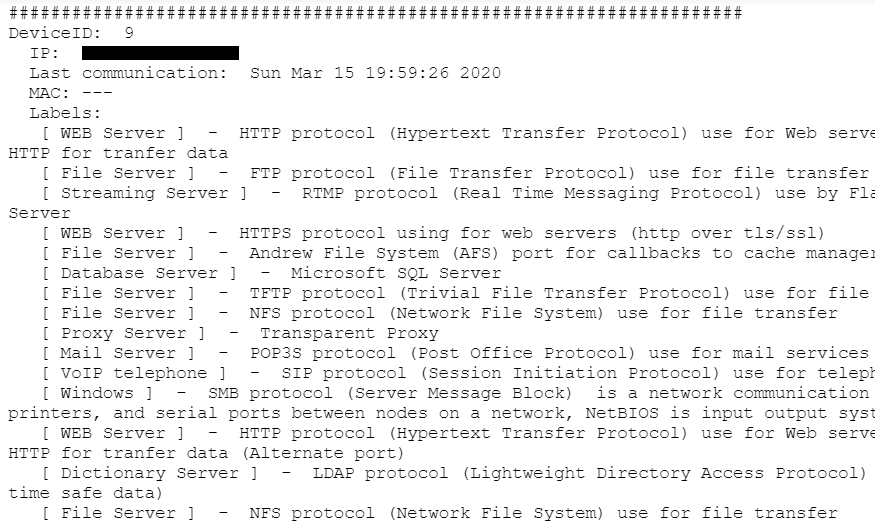
\includegraphics[width=\textwidth]{Global_nondelete}
        \caption[Ukázka měření: Globální síť]{Zařízení v globální síti}
        \label{Global1}
    \end{figure}
    
    Okamžitě si všimneme velkého počtu štítků, přičemž závislosti zodpovědné za tyto štítky mají většinou malý počet paketů. Z toho vyvodíme, že tyhle závislosti jsou vytvořené roboty, které prohledávají aktivním způsobem globální rozsahy IP adres za účelem zjišťování, jaké služby zařízení na daných IP adresách poskytují. Abychom tyto závislosti odstranili a tím zpřesnili měření, musíme při spouštění našeho modulu přidat parametr \emph{-D} spolu s počtem paketů, jenž slouží jako hranice pro vymazání závislosti. 
    
    Na Obrázku \ref{Global2} je vyobrazen výstup analýzy při periodickém mazaní globálních závislostí. 
    \begin{figure}[h!]
        \centering
        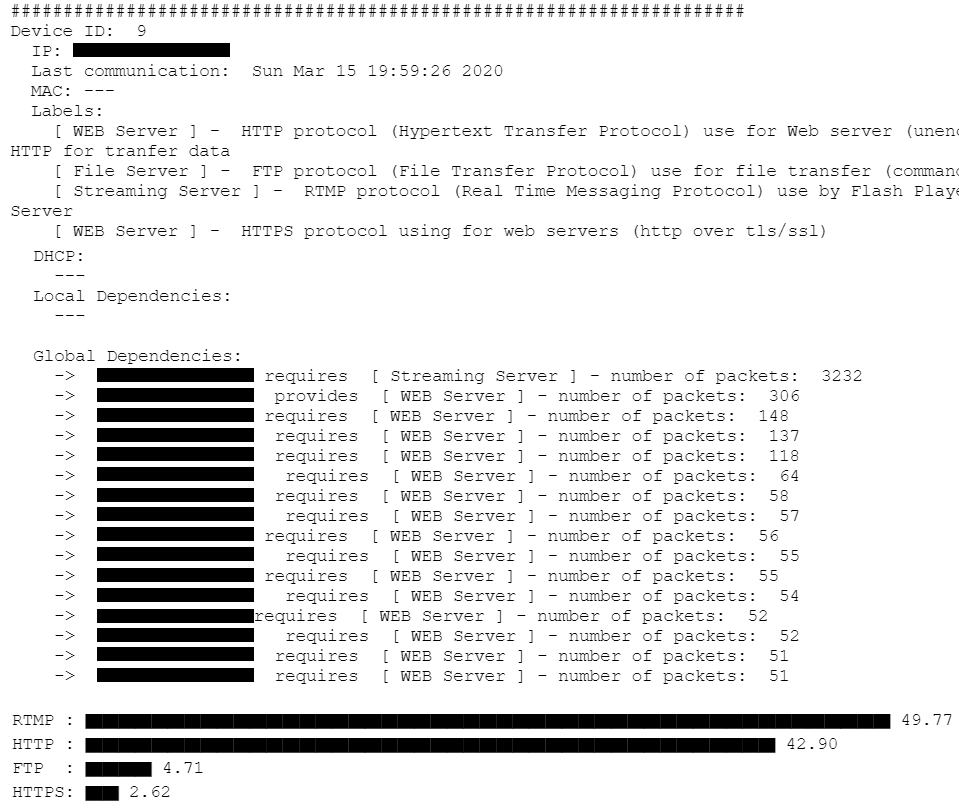
\includegraphics[width=\textwidth]{Global_delete_5}
        \caption[Ukázka měření: Globální síť s periodickým mazáním závislostí]{Zařízení v globální síti při mazání závislostí}
        \label{Global2}
    \end{figure}
    
    Mazání závislostí s pěti a méně pakety výrazně snížilo počet štítků. Ale periodické mazání závislostí ne vždy bude fungovat. Záleží na zvoleném počtu paketů a také komunikaci, která probíhá během jedné periody (10\,000 IP flows). Pokud v jedné periodě bude jeden robot vícekrát analyzovat dané zařízení, potom závislosti tím vzniklé mohou mít více paketů než je zvolené hranice. Tím pádem budou štítky nepřesné.
    
    Proto zkusíme analyzovat každý IP flow s cílem pracovat pouze s úplnými závislostmi. To znamená, že pokud jedno zařízení komunikuje směrem na druhé zařízení pod nějakým specifickým protokolem z tabulky \emph{Services} a druhé zařízení na jeho požadavky neodpovídá, vznikne neúplná závislost. Přidáním parametru \emph{-F} spustíme filtrování IP flows. Výsledek filtrování TCP a UDP provozu můžeme vidět na Obrázku \ref{Global3}
    
    \newpage
    \begin{figure}[h!]
        \centering
        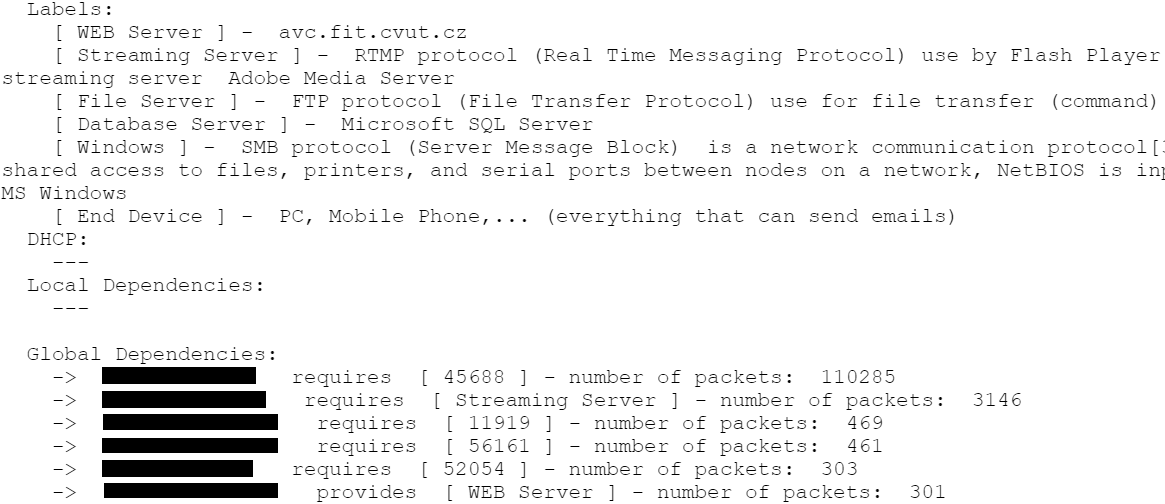
\includegraphics[width=\textwidth]{Global_filter.png}
        \caption[Ukázka měření: Globální síť s filtrováním závislostí]{Zařízení v globální síti při filtrování závislostí}
        \label{Global3}
    \end{figure}
    
    Ze štítků z Obrázků \ref{Global2} a \ref{Global3}  a ze závislostí můžeme odhadnout, že dané zařízení je server poskytující webový server, na kterém lze přehrávat videa za použití \emph{RTMP} protokolu.
    
    Ověříme si výsledek přeložením IP adresy na doménové jméno a získáme \emph{avc.fit.cvut.cz}. Což je web zaměřený na nahrané přednášky Fakulty Informačních Technologií na ČVUT, které lze na tomto webu přehrát. Štítkování v tomto konkrétním příkladě bezpečně odhalilo úlohu zařízení na této IP adrese. 
    
    V dalších příkladech můžeme uvést zařízení, kterému náš modul přiřadil štítky \emph{WEB Server} a \emph{Mail Server}. Doménové jméno tohoto zařízení je \emph{imap.fit.cvut.cz}, což je webový e-mailový klient FIT ČVUT. Dále jsme nalezli zařízení se štítky \emph{Router} a \emph{End Device}, jenž ukazuje na router, za kterým se nachází lokální síť. 
    
    
    %Také jsme nalezli více zařízení používající RSTP protokol, který se používá u IP kamer nebo přenosu steamovacích služeb.
    \newpage
    \section{Časová náročnost}
    \subsection{PassiveAutodiscovery modul}
    V našem případě časová náročnost či složitost neurčuje, za jak dlouho program doběhne, ale spíše ukazuje jak dlouho a při jakém množství komunikace je modul schopen pracovat při běhu na síti.
    
    Pro odhadnutí časové náročnosti nám velice dobře postačí hodinový záznam globální sítě popsané v předchozí podkapitole. V těchto záznamech se nachází 418\,647 IP flows a v naší tabulce \emph{Global}, kde se nachází pouze jedinečné závislosti, to vyplní přes 80\,000 záznamů. Objem komunikace za tuto hodinu je tedy značný a bude postačovat pro odhadnutí časových náročností našeho modulu při různých nastaveních pomocí parametrů. Měření jsme prováděli na notebooku HP ProBook 4720s s procesorem Intel i3 M 350 2.2\,GHz, RAM pamětí 4\,GiB DDR3 a s SSD diskem s rychlostí čtení 	500\,MB/s a zápisu 320\,MB/s. 
    
    Jak jsme již řešili v kapitole \emph{Návrh} zvolená databáze \emph{sqlite3} je oproti klasickým databázovým serverům pomalejší, jelikož po každém vložení či úpravě záznamu v databázi čeká, než se krok propíše do souboru \emph{.db} představující databázi. Z toho důvodu řádně otestujeme, zda a jak to omezuje měření v síti, a výsledky měření porovnáme s variantou průběžného ukládání celé \emph{sqlite3} databáze do RAM paměti. Tato varianta by měla urychlit vkládání a úpravy záznamů v databázi.
    
    Zahájili jsme na tomto hodinovém záznamu měření s cílem zjistit časovou náročnost pro různé nastavení modulu pomocí parametrů. Výsledky všech měření jsou přehledně zobrazené v Tabulce \ref{TabMereni}. Všimněme si, že nejvíce časovou náročnost zlepšuje parametr \emph{-RAM}, díky kterému se v průběhu měření celá \emph{sqlite3} databáze ukládá do RAM paměti a do souboru se zapíše naráz na konci měření. Dalším parametrem, který měření urychlí je \emph{-D}, který průběžně promazává tabulku \emph{Global} od závislostí, které mají menší počet paketů než je zadaný počet. Tím může uživatel smazat \uv{nepodstatné} závislosti.
    
    Když jsme testovali modul v reálných lokálních sítích, tak jsme nezaznamenali s měřením žádné časové problémy, ale objem komunikace na těchto sítích nebyl velký, a tak jsme si mohli dovolit informační výpisy z \emph{PassiveAutodiscovery.py}. Avšak na tomto velkém hodinovém záznamu trvají pouhé výpisy nově nalezených zařízení, závislostí a dalších informací přes jednu hodinu. Při používání modulu na velkém provozu je proto nutné zvážit vypnutí výpisů pro zvýšení výkonu. Výkonnostní optimalizace modulu jsou nad rámec této bakalářské práce a jsou ponechány jako budoucí práce. 
    
    
    \begin{table}[h]\centering
 	    \caption[Tabulka časových měření: PassiveAutodiscovery modul]{Tabulka měření času zpracování v hodinách a minutách v závislosti na zvolených parametrech.}\label{TabMereni}
 	    \begin{tabular}{|>{\centering}m{5.5cm}|c|c|}\hline
 		\textbf{Způsob měření}		                    & \textbf{Přepínače modulu} & \textbf{Čas měření} \tabularnewline \hline \hline
 		S informačními výpisy		            & 	-G -l -s -L -m -S -g	& 3:30	\tabularnewline \hline
 		Bez informačních výpisů		            & 	-G	                    & 2:37	\tabularnewline \hline
 	    Pouze \uv{běžné} porty		            & 	-G -U                   & 1:20	\tabularnewline \hline
 	    S odstraňováním globálních závislostí 	& 	-G -U -D 5              & 0:47	\tabularnewline \hline
 	    Bez ukládání globálních závislostí      &   -U                      & 0:37	\tabularnewline \hline
 	    Pouze \uv{běžné} porty s používáním RAM paměti    &   -G -U -RAM    & 0:24	\tabularnewline \hline
 	    Filtrování neúplných závislostí s používáním RAM paměti  & 	-G -F -RAM              & 0:21	\tabularnewline \hline
 	    S odstraňováním globálních závislostí a s používáním RAM paměti 	& 	-G -U -D 5 -RAM & 0:13	\tabularnewline \hline
 	    Bez ukládání globálních závislostí a s použitím RAM paměti   &   -U -RAM & 0:05	\tabularnewline \hline
 	    \end{tabular}
    \end{table}
    \newpage
    \subsection{DeviceAnalyzer}
    Čas běhu \emph{DeviceAnalyzer} skriptu záleží na počtu záznamů v databázi a na použitých parametrech, protože některé výrazně zpomalí běh analýzy. Pro ukázku, jak je časová náročnost ovlivňována parametry, jsme použili záznam kancelářské sítě z druhého testování. Výsledky měření jsme zapsali do přehledné Tabulky \ref{TabMereniD}.
    
    Z tabulky vidíme, že nejvíce náročným parametrem je \emph{-DNS}, který překládá každou IP adresu označenou štítkem \emph{WEB Server} na doménové jméno, pokud to lze. Dalším výrazným parametrem je \emph{-G číslo} (respektive \emph{-L číslo}), který ve výstupu omezuje počet globálních (respektive lokální) závislostí. Čímž zlepší časovou náročnost.
    \newpage
    \begin{table}[h]\centering
 	    \caption[Tabulka časových měření: DeviceAnalyzer skript]{Tabulka měření času analyzování v hodinách a minutách v závislosti na zvolených parametrech.}\label{TabMereniD}
 	    \begin{tabular}{|>{\centering}m{5,5cm}|c|c|}\hline
 		\textbf{Způsob měření}		                    & \textbf{Přepínače modulu} & \textbf{Čas měření} \tabularnewline \hline \hline
 		Překlad DNS a neomezené globální závislosti	s výstupem do příkazové řádky a tvorbou grafů	            & 	-p -DNS -l -g	& 5 m 31.12 s	\tabularnewline \hline
 		Překlad DNS a neomezené globální závislosti	s výstupem do souboru a tvorbou grafů		            & 	-f file -DNS -l -g	& 5 m 11.12 s	\tabularnewline \hline
 		Překlad DNS a neomezené globální závislosti	s výstupem do příkazové řádky		            & 	-p -DNS	& 4 m 52.34 s	\tabularnewline \hline
 		Překlad DNS a neomezené globální závislosti	s výstupem do souboru		            & 	-f file -DNS	& 4 m 48.46 s	\tabularnewline \hline
 		Překlad DNS a omezené globální závislosti	s výstupem do příkazové řádky a tvorbou grafů		            & 	-p -DNS -l -g -G 15	& 2 m 49.68 s	\tabularnewline \hline
 		Překlad DNS a omezené globální závislosti	s výstupem do souboru a tvorbou grafů	            & 	-f file -DNS -l -g -G 15	& 2 m 36.87 s	\tabularnewline \hline
 		Omezené globálních závislostí s výstupem do příkazové řádky a tvorbou grafů		            & 	-p -l -g -G 15	& 2 m 43.16 s	\tabularnewline \hline
 		Omezené globálních závislostí s výstupem do souboru a tvorbou grafů			            & 	-f file -l -g -G 15	& 2 m 42.30 s	\tabularnewline \hline
 		Neomezené globálních závislostí s výstupem do příkazové řádky a tvorbou grafů		            & 	-p -l -g	& 2 m 17.93 s	\tabularnewline \hline
 		Neomezené globálních závislostí s výstupem do souboru a tvorbou grafů		            & 	-f file -l -g	& 2 m 12.92 s	\tabularnewline \hline
 		Pouze lokální závislosti s výstupem do příkazové řádky		            & 	-p -o	& 2.45 s	\tabularnewline \hline
 		Pouze lokální závislosti s výstupem do souboru		            & 	-f file -o	& 2.28 s	\tabularnewline \hline
 		
 	    \end{tabular}
 	\end{table}
 	\newpage
    
    \section{Paměťová náročnost}
    \subsection{PassiveAutodiscovery modul}
    Paměťová náročnost \emph{PassiveAutodiscovery} modulu je závislá na způsobu uložení \emph{sqlite3} databáze a počtu záznamů do ní uložených. Pro odhadnutí a vykreslení této náročnosti jsme použili záznam globální sítě z předchozí ukázky. Na Obrázku \ref{PAMU1} vidíme, že paměťová náročnost při uložení databáze do souboru je rostoucí v závislosti na počtu vložených dat do databáze. V druhé polovině měření již velká část zařízeních, služeb a závislostí v databázi již existovalo, proto množství alokované paměti stoupalo pomaleji.
    \begin{figure}[h!]
        \centering
        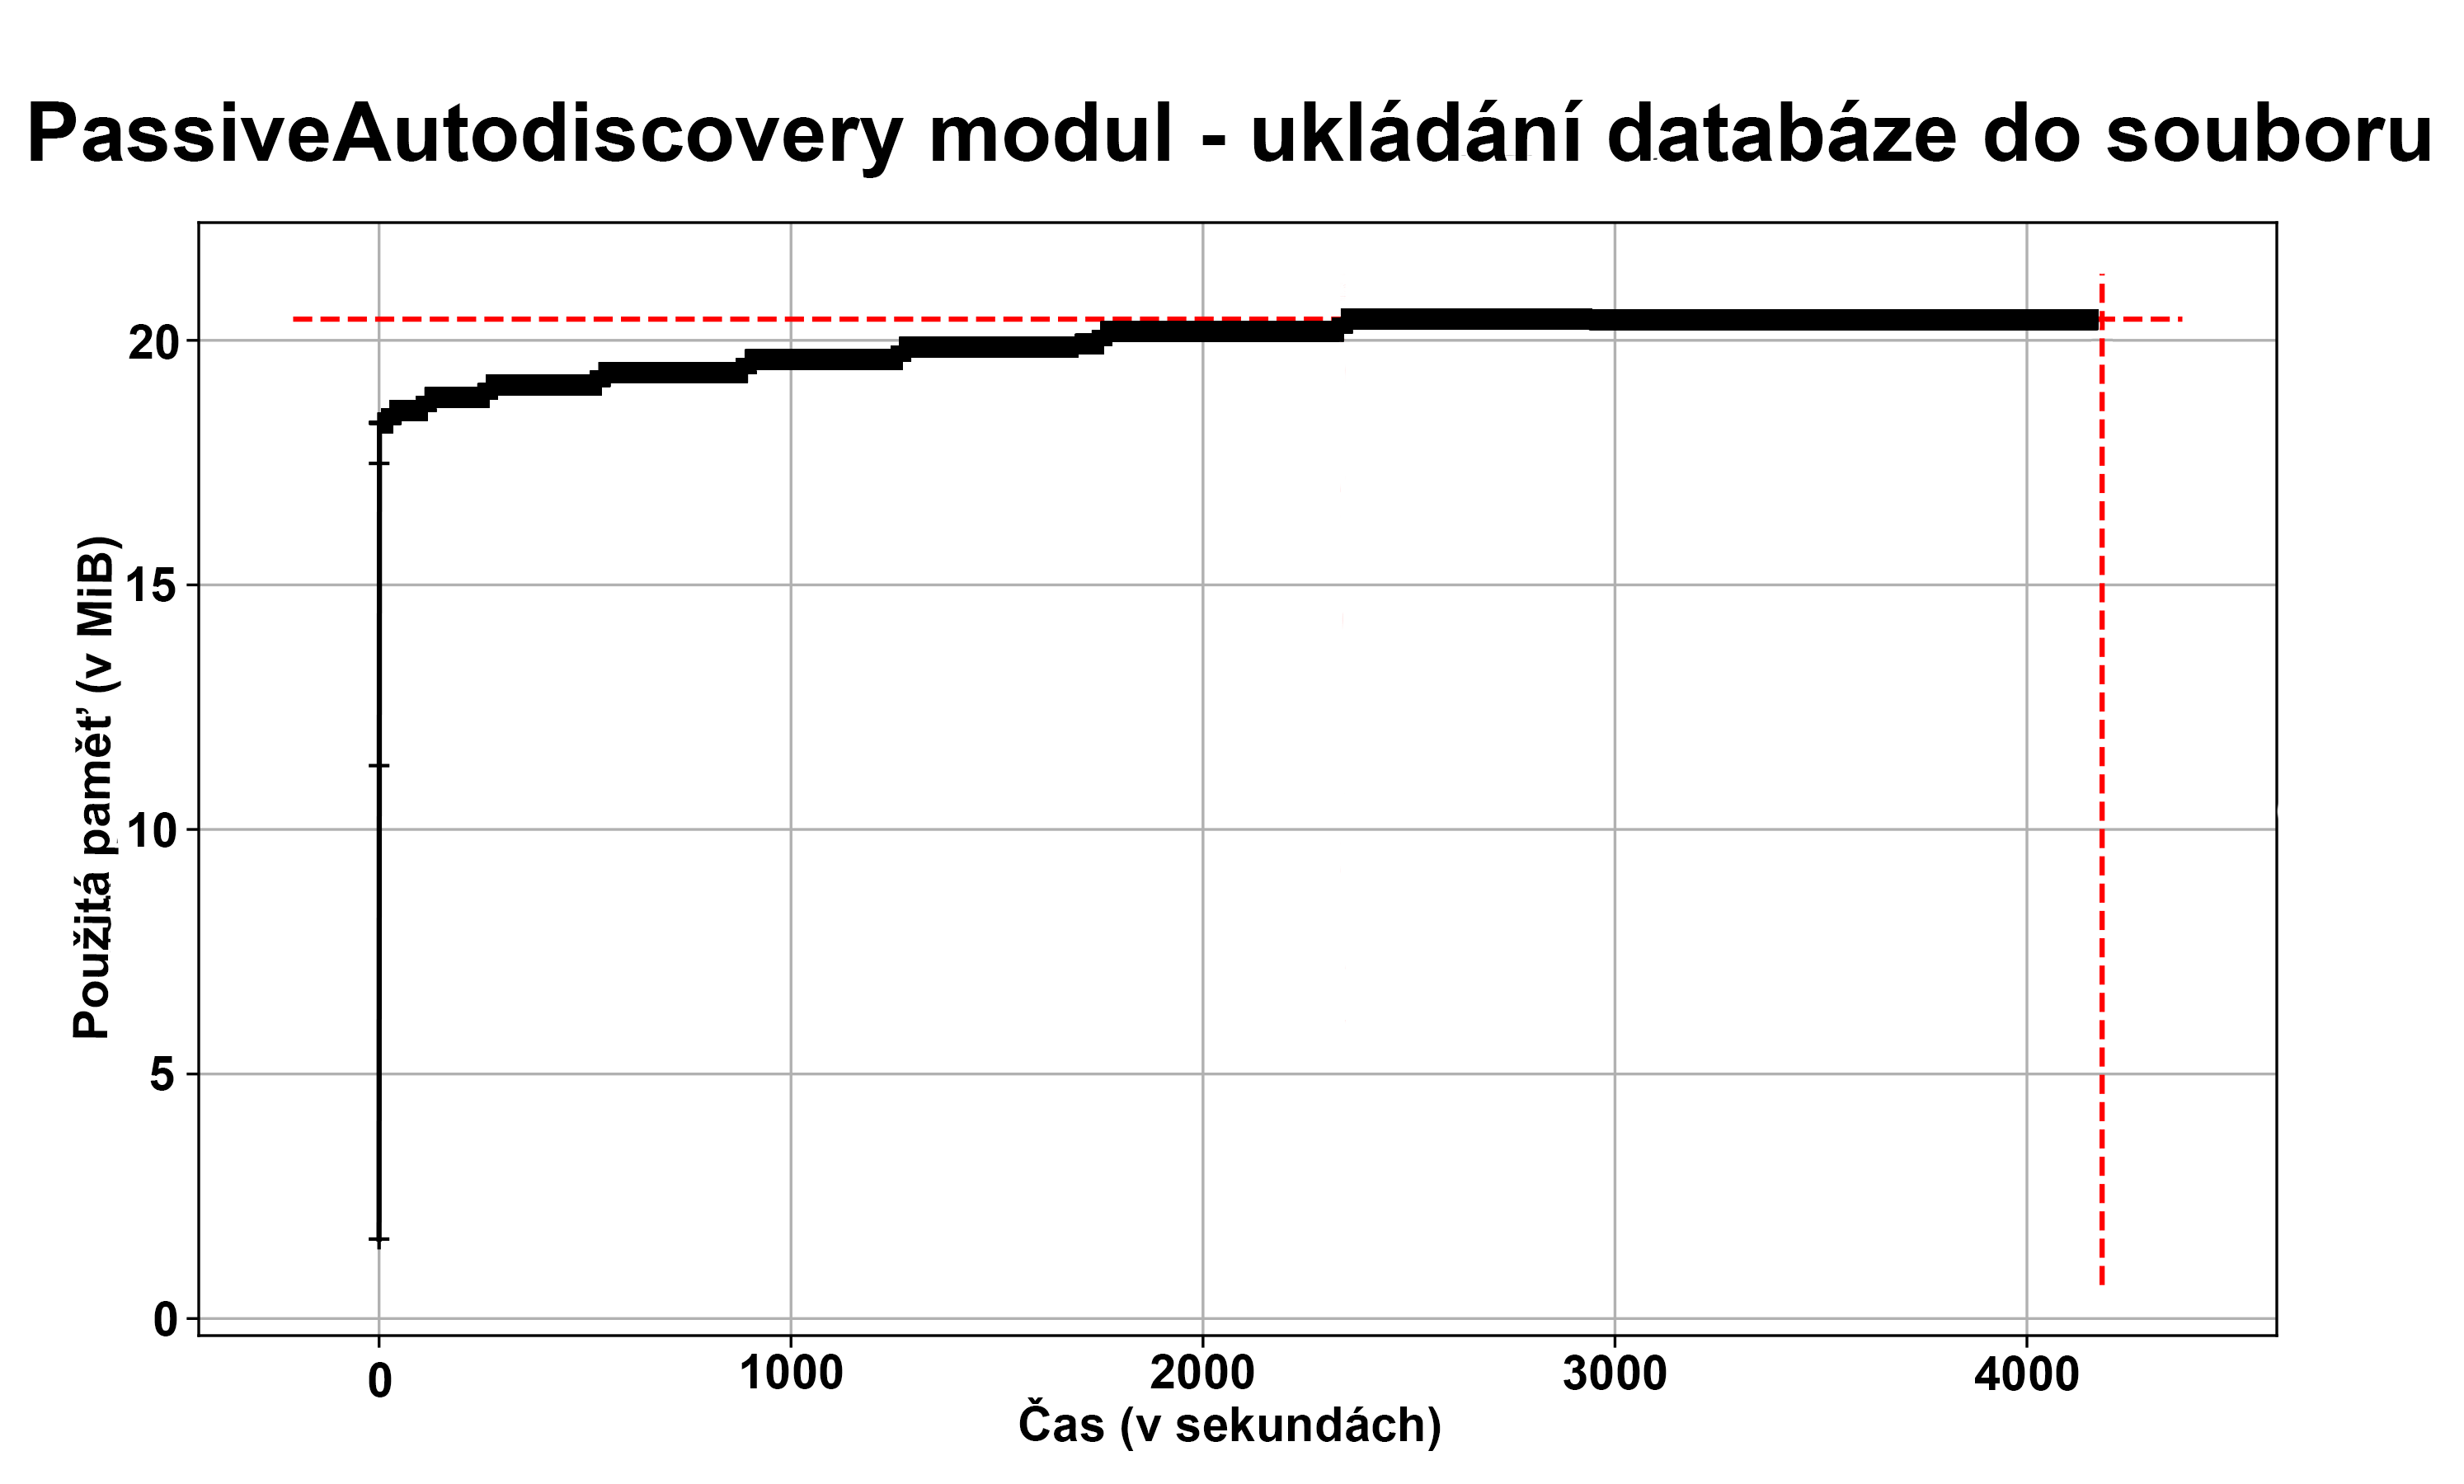
\includegraphics[width=\textwidth]{GlobalFile.png}
        \caption[Paměťová náročnost: PassiveAutodiscovery modulu s uložením databáze v souboru]{PassiveAutodiscovery modulu s uložením databáze v souboru}
        \label{PAMU1}
    \end{figure}
    
    Na druhém Obrázku \ref{PAMU2} je naopak znázorněna paměťová náročnost při ukládání databáze do RAM paměti. Na první pohled si všimneme, že se využití paměti zvýšilo o velikost databáze a na konci běhu modulu využití vzrostlo. To je způsobené tím, že se na konci přenáší databáze z RAM paměti do souboru. Paměťová náročnost po většinu doby je stejně jako při ukládání databáze do souboru rostoucí v závislosti na počtu vložených dat do databáze. 
    \begin{figure}[h!]
        \centering
        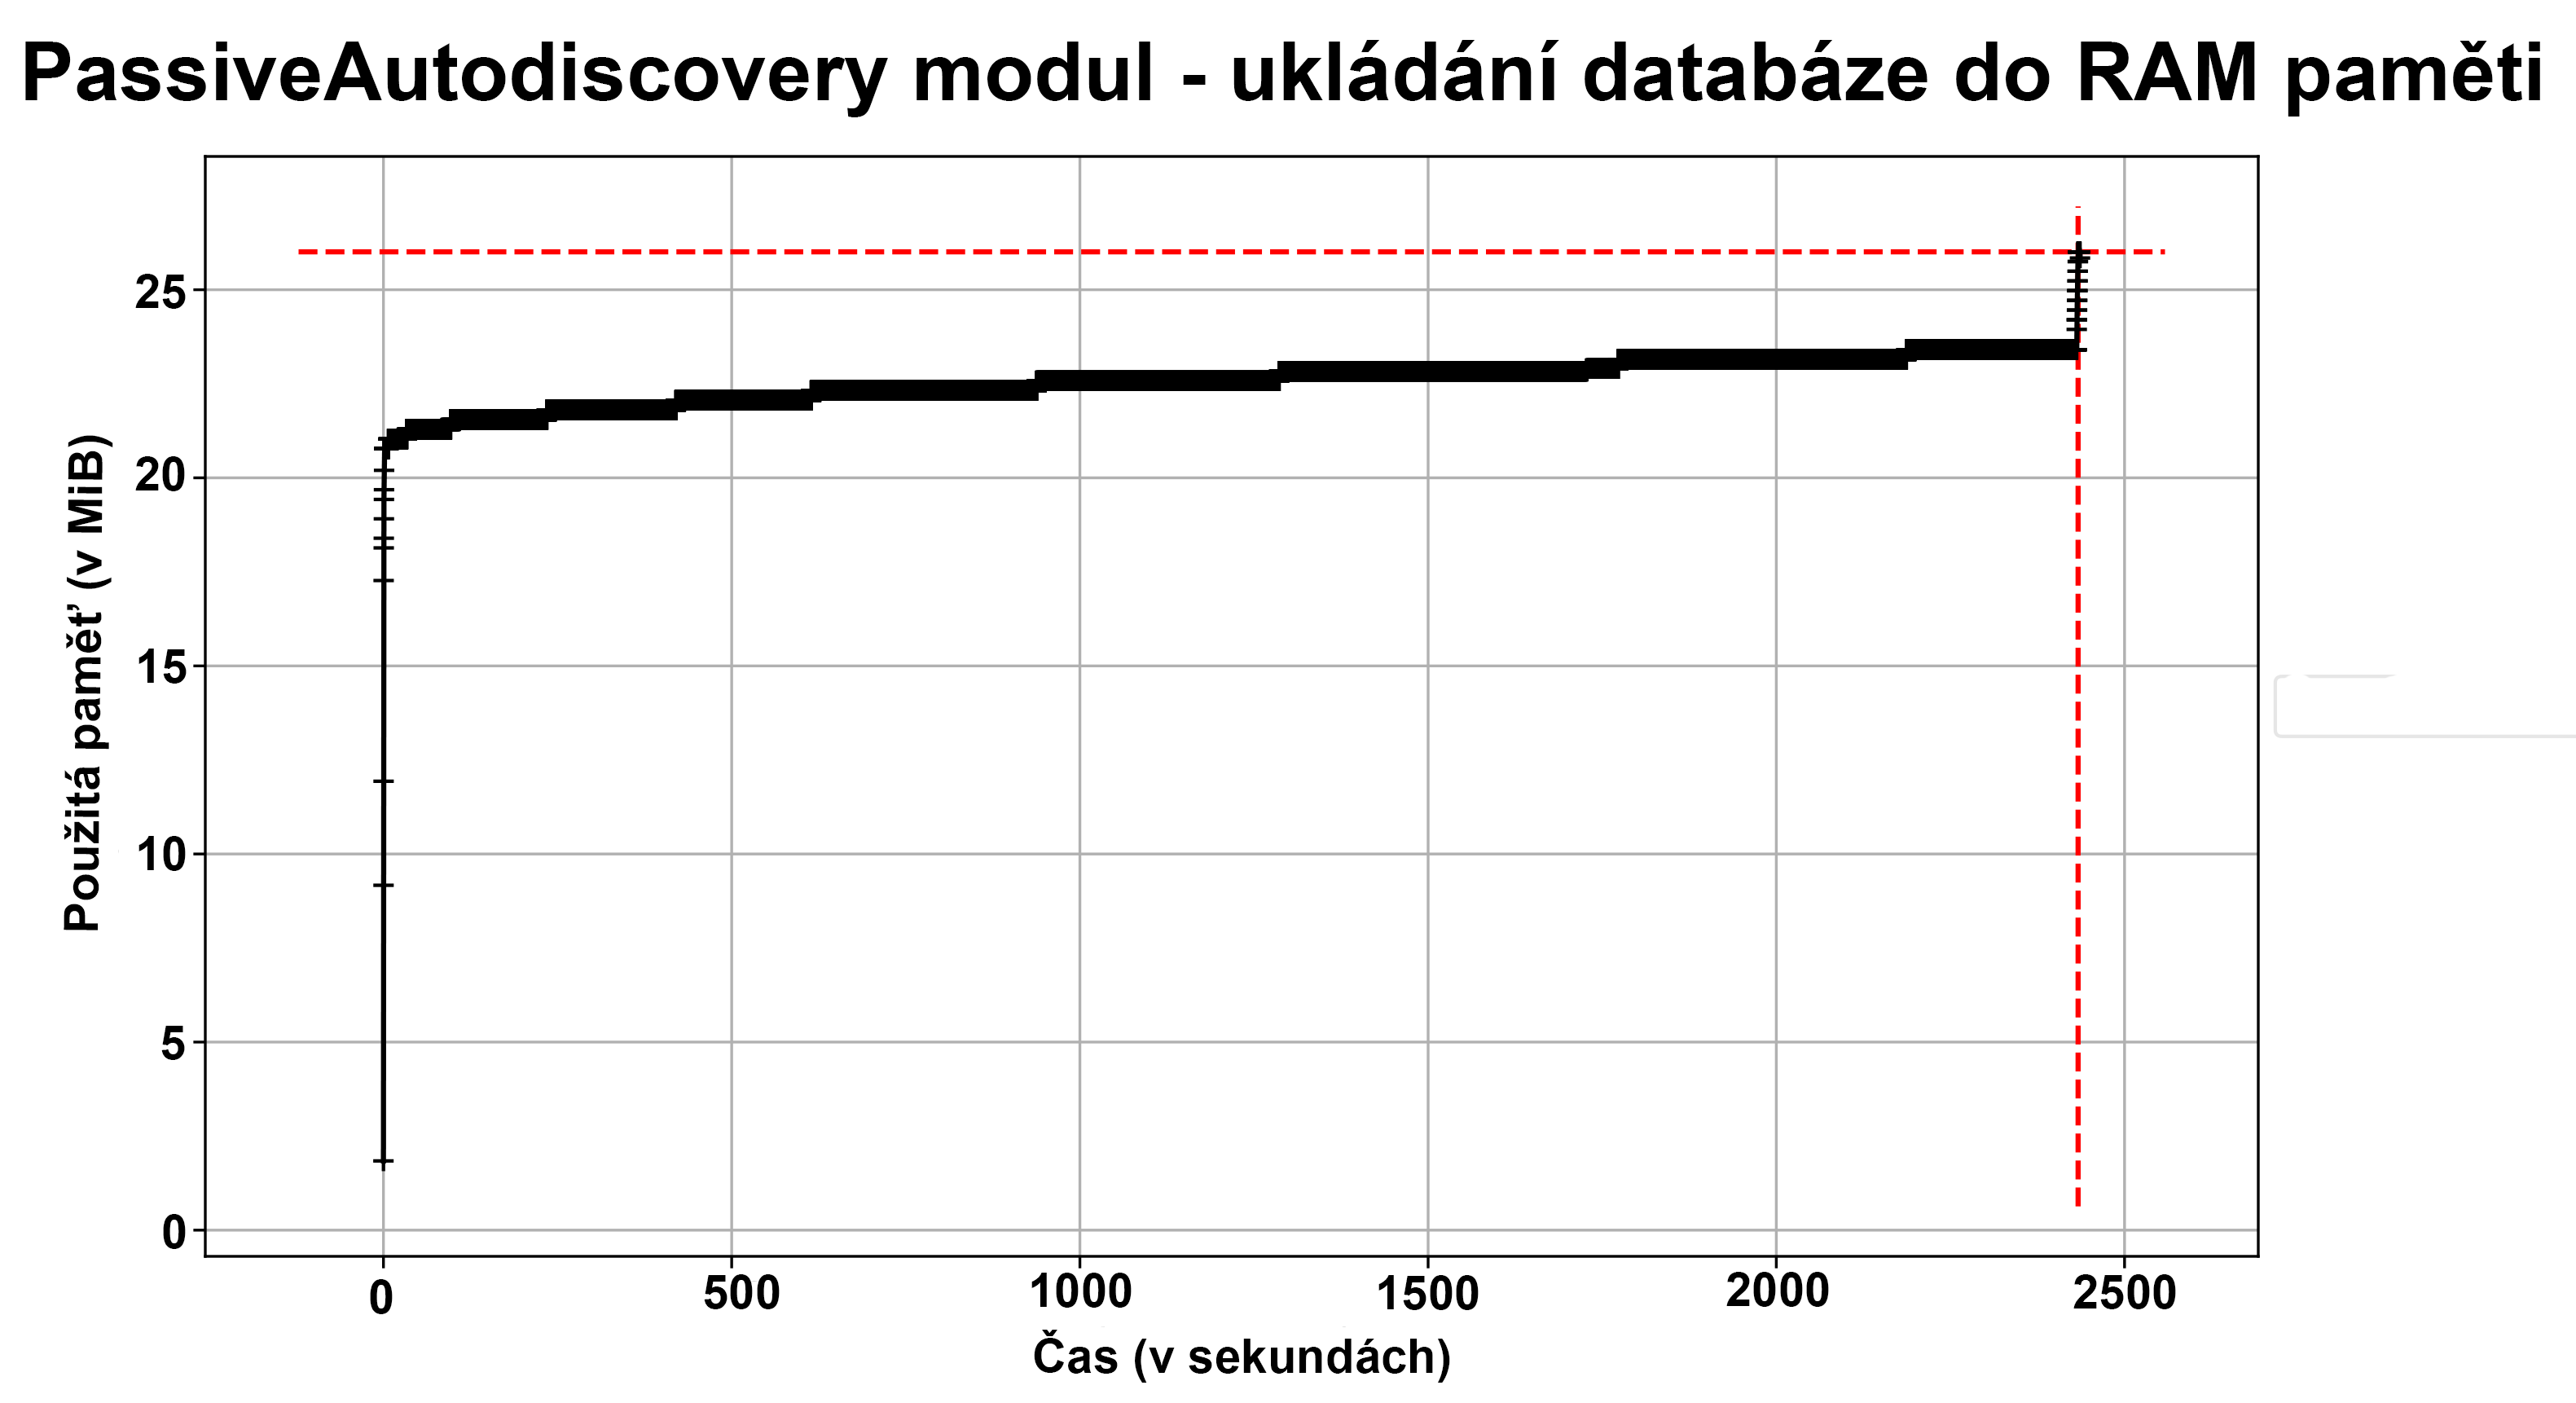
\includegraphics[width=\textwidth]{GlobalRAM.png}
        \caption[Paměťová náročnost: PassiveAutodiscovery modulu s uložením databáze v RAM paměti]{Paměťová náročnost PassiveAutodiscovery modulu s uložením databáze v RAM paměti}
        \label{PAMU2}
    \end{figure}
    
    \newpage
    \subsection{DeviceAnalyzer}
    U \emph{DeviceAnalyzer} skriptu ukážeme vývoj paměťové náročnosti na dvou grafech, ve kterých porovnáme využití paměti v závislosti na velikosti analyzované databáze.
    
    Na Obrázku \ref{DAMU1} je vykresleno využití paměti při analýze domácí sítě z první ukázky testování. Všimněme si, že většinu běhu skriptu byla náročnost konstantní a na konci běhu se zvýšila při vykreslování grafů závislostí a statistiky využití sítě zařízeními.
    
    Na druhém Obrázku \ref{DAMU2} je k porovnání zobrazen vývoj paměťového využití skriptem při analýze globální sítě z druhé ukázky, která v porovnání s druhým modulem má mnohonásobně větší vstupní databázi k analýze. Zajímavostí je vývoj, který je během běhu lehce rostoucí a na konci skriptu je taktéž zvýšení při vykreslování grafů a statistiky.
    
    Přestože vstupní databáze byla v druhém příkladě mnohanásobně větší, tak se paměťové využití příliš nezvýšilo a ono zvýšení je způsobeno počtem zařízení a informací o nich, které se průběžně ukládají do výstupního JSON dokumentu. Z toho vyvodíme, že vstupní databáze příliš neovlivňuje paměťovou náročnost a paměťová náročnost je lehce rostoucí jelikož se výstup DeviceAnalyzer skriptu průběžně ukládá do JSON dokumentu, který je průběžně ukládán do RAM paměti.
    
    \begin{figure}[h!]
        \centering
        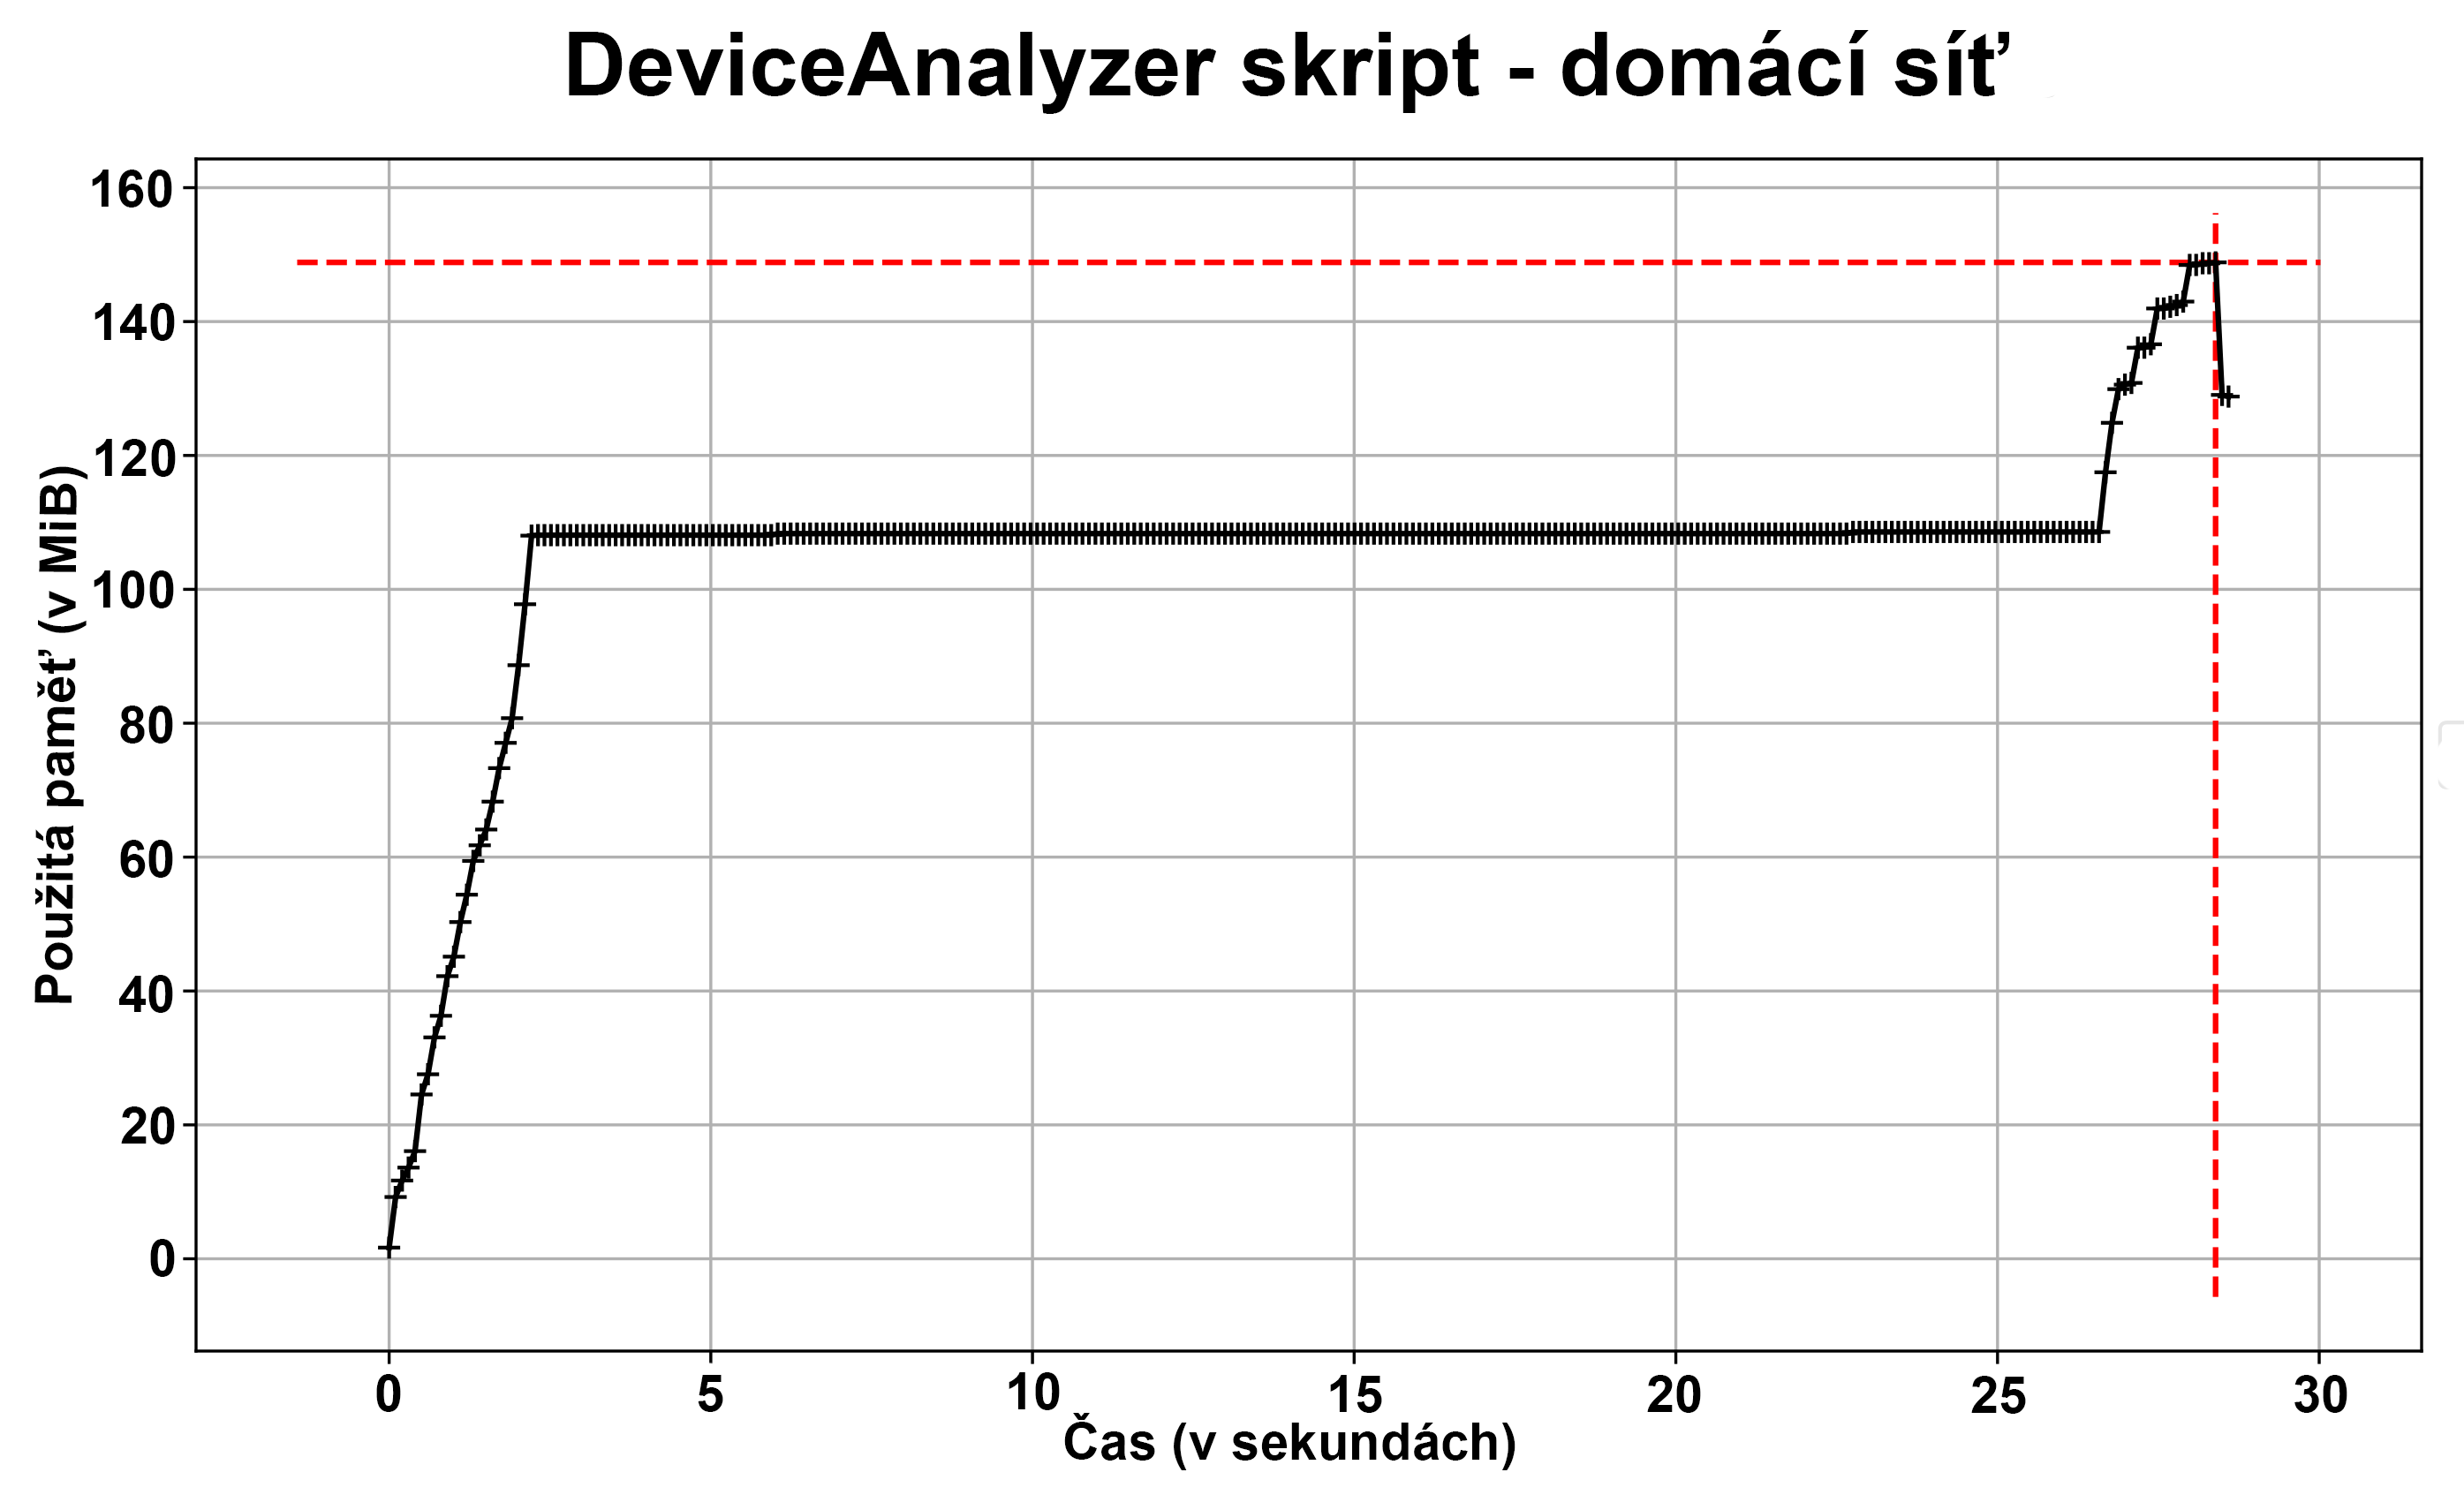
\includegraphics[width=\textwidth]{DeviceAnalyzerMemoryUsage.png}
        \caption[Paměťová náročnost: DeviceAnalyzer skriptu na domácí síti]{Paměťová náročnost DeviceAnalyzer skriptu na domácí síti}
        \label{DAMU1}
    \end{figure}
    \begin{figure}[h!]
        \centering
        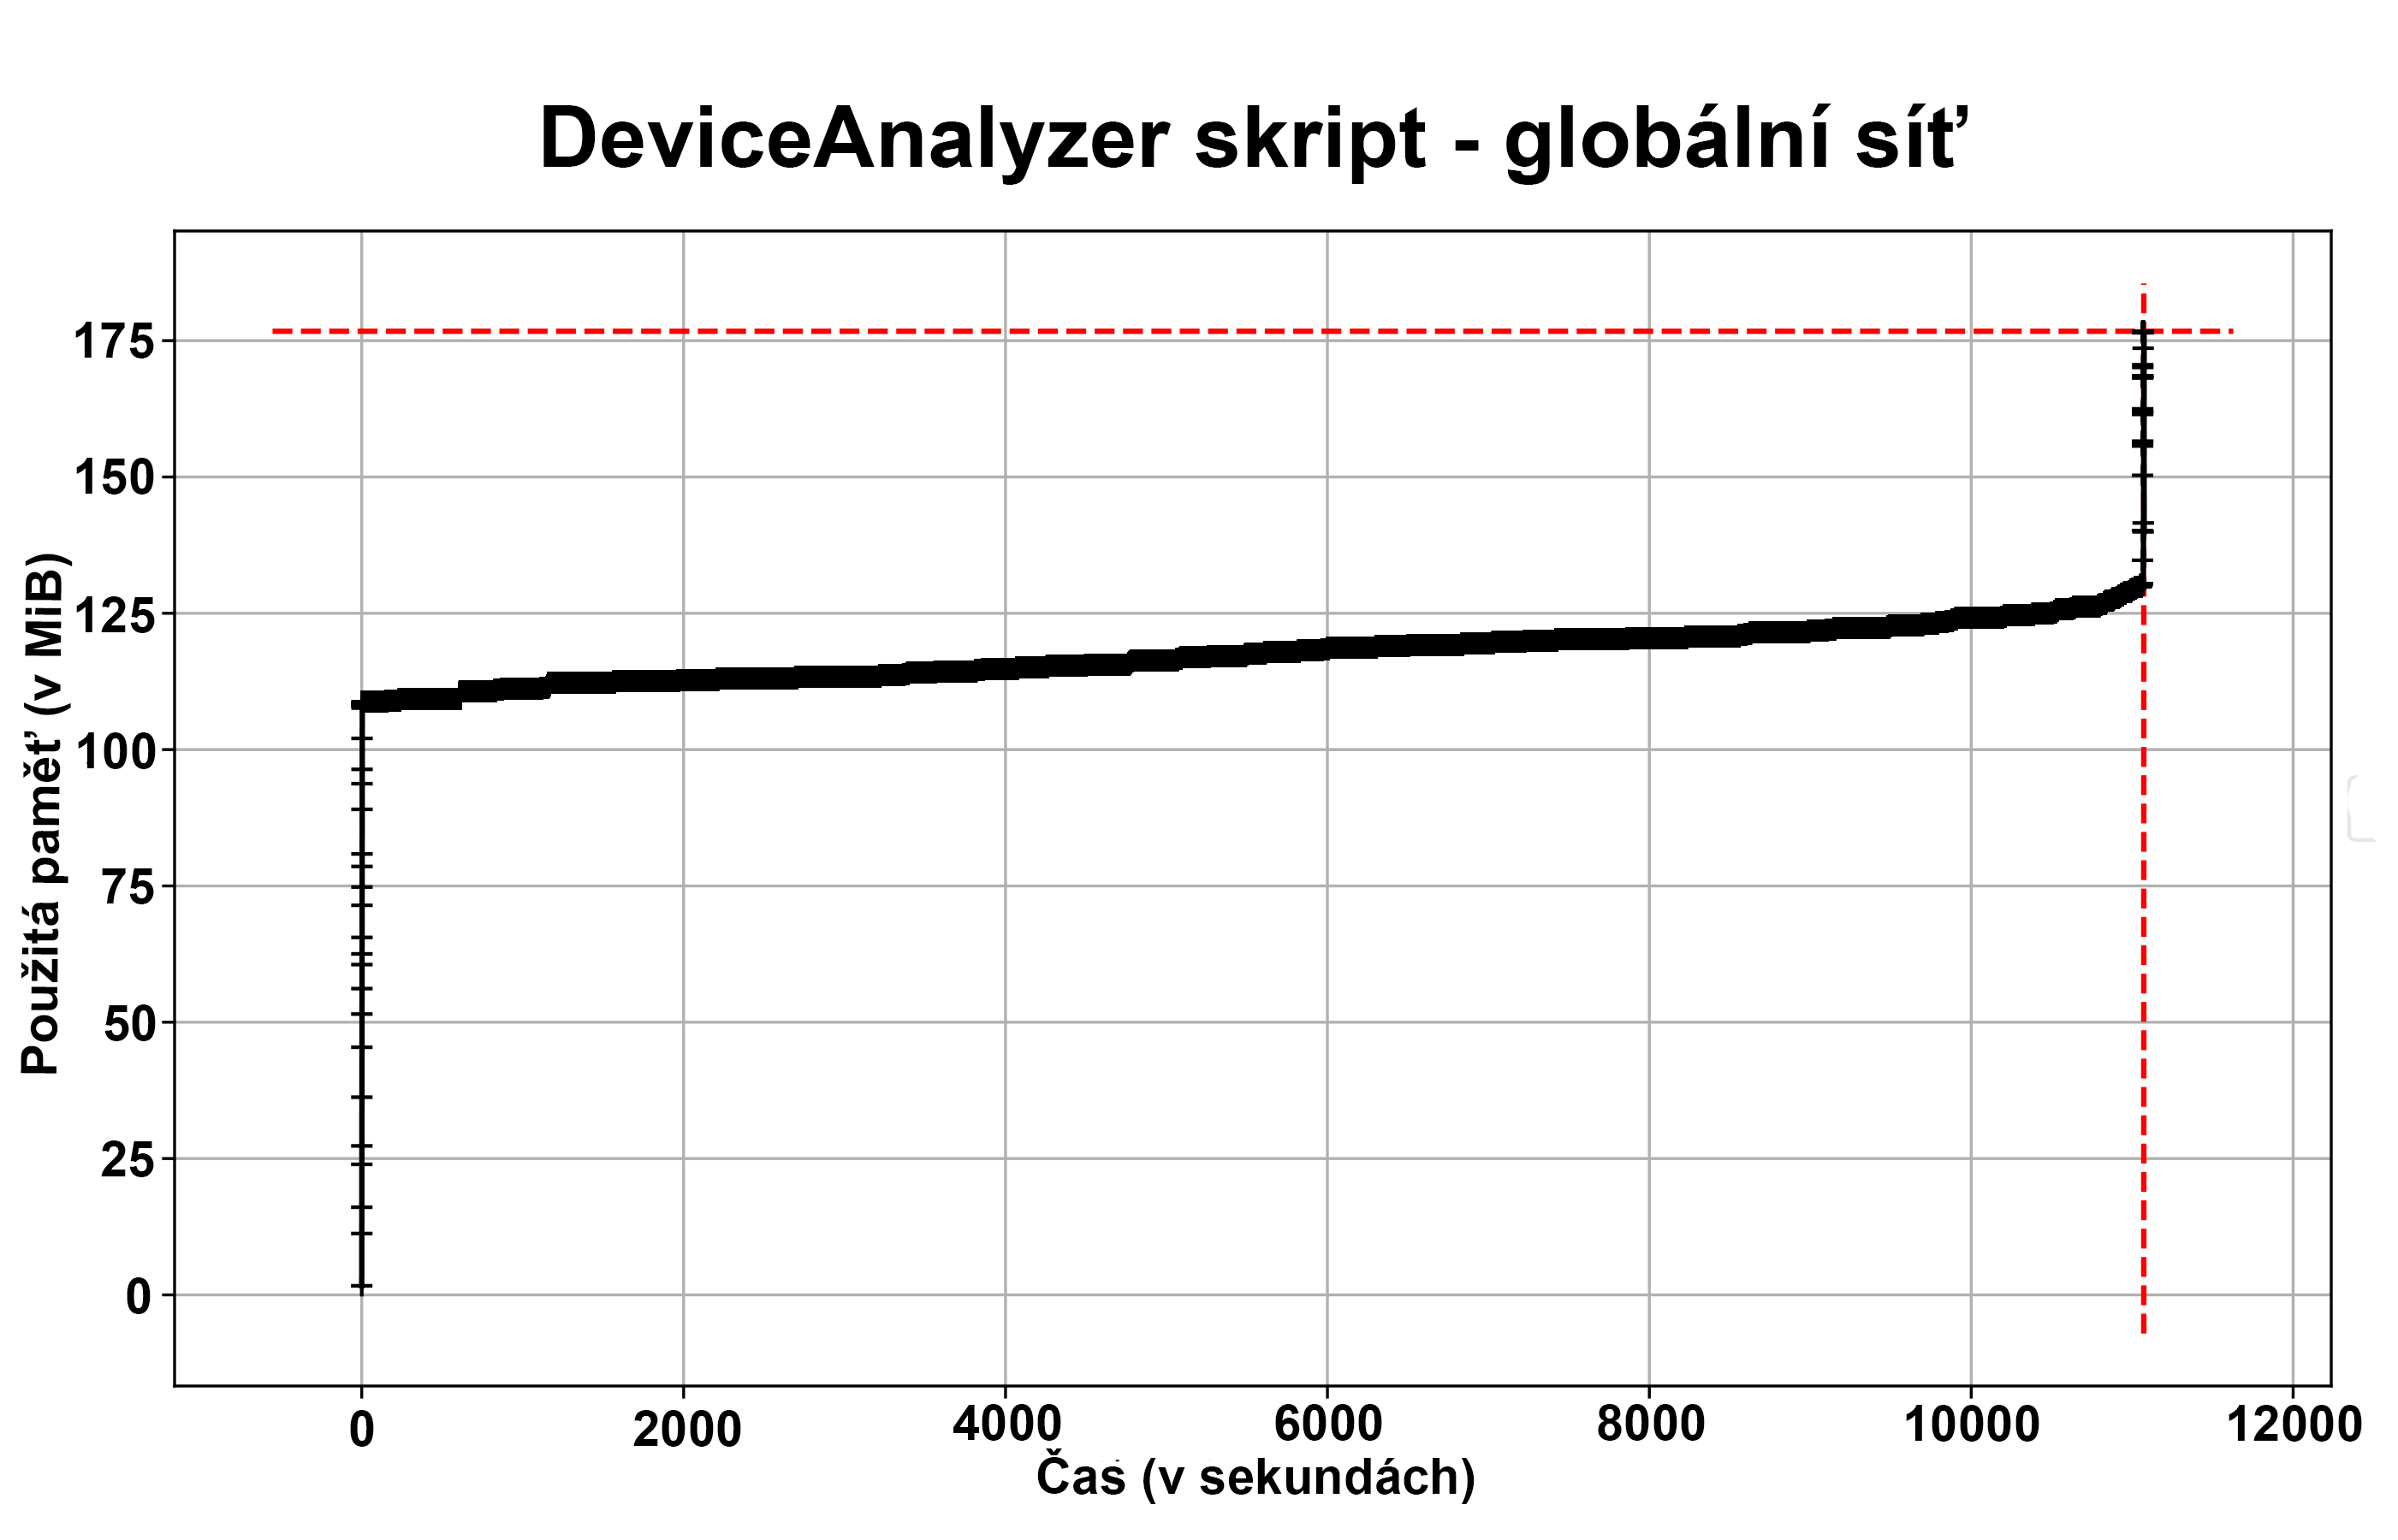
\includegraphics[width=\textwidth]{GlobalDeleteMemoryUses.png}
        \caption[Paměťová náročnost: DeviceAnalyzer skriptu na globální síti]{Paměťová náročnost DeviceAnalyzer skriptu na globální síti}
        \label{DAMU2}
    \end{figure}

%===========================================================================================================
%===========================================================================================================
%===========================================================================================================


\begin{conclusion}
	Naším hlavním cílem bylo vytvořit seznam štítků, které určují roli zařízení v síti, a tyto štítky následně automaticky přiřazovat fyzickým zařízením na základě jejich provozu na síti. Tímto způsobem je možné zmapovat libovolnou síťovou infrastrukturu na základě pasivně pozorovaného síťového provozu. Dále jsme měli zajistit ukládání závislostí mezi zařízeními a ty následně vizualizovat pomocí grafů. 
	
	V rámci této bakalářské práce byl vytvořen prototyp softwarového modulu, který dokáže na základě síťových toků zmapovat aktivní zařízení, získat o nich detailnější informace a  rozpoznávat závislostí mezi poskytovanými službami a klienty na síti. Prototyp byl implementován jako modul do modulárního systému NEMEA. Výsledná aplikace byla následně otestována na reálném síťovém provozu a proběhlo měření výkonu a potřebné alokované paměti.
	
	Z dostupných zdrojů se nám podařilo vytvořit seznam štítků rolí s jejich specifickými či často používanými protokoly transportní vrstvy TCP/IP modelu. Ve vytvořeném seznamu je přes 40 různých štítků a přes 250 protokolů k nim přiřazeným.
	
	Navrhli a implementovali jsme databázi, která obsahuje počáteční údaje pro náš modul včetně seznamu štítků. Do této databáze náš modul ukládá nasbíraná data, se kterými následně pracuje skript pro analýzu. Díky spolupráci s databází jsme dokázali v modulu implementovat přiřazování štítků jednotlivým zařízením pomocí jednoduchých dotazů, evidovat závislostí mezi zařízeními a jejich přístupy do internetu či záznamy o DHCP komunikaci. Vytvořili jsme skript, který naší databázi projde a vytvoří výstupní analýzu. Ta předně obsahuje pro každé fyzické zařízení přiřazené štítky a závislosti s ostatními zařízeními. Skript taktéž vytvoří graf závislostí mezi zařízeními, který uloží do souboru. 
	
	Modul je primárně určený pro lokální sítě, ale vhodně jsme ho rozšířili, aby byl schopen fungovat i na sítích globálních, přičemž výsledky testování na globálních sítích jsou dostačující pro přehled o rolích daných zařízení. Naše zvolená databáze má omezení, které způsobuje pomalejší vkládání a upravování dat v databázi, ale dokázali jsme implementovat ukládání do RAM paměti, které toto omezení zmenšuje, přičemž jsme při měření časové složitosti dokázali jeho funkčnost.
	
	\section{Možný budoucí vývoj}
	V rámci projektu ADiCT (Asset Discovery Classification Tagging) pod sdružením CESNET bude vytvořená centrální databáze, která bude shromažďovat informace o zařízeních (především serverech) v síti. Moduly vyvinuté v rámci této bakalářské práce se stanou jedním ze zdrojů primárních dat pro znalostní databázi. Proto proběhne v budoucnu předělání tohoto modulu pro práci s touto nově vzniklou jednotnou databází.
	
	Ve skriptu pro analýzu jsme implementovali výstup ve formátu JSON dokumentu s cílem dlouhodobého uložení analýzy do souboru, se kterým může snadno pracovat jakýkoliv program či skript. Je předlohou pro možnou budoucí aplikaci, která by z tohoto výstupního JSON dokumentu mohla graficky prezentovat získané informace o zařízeních.
	
	
	
	
\end{conclusion}
%===========================================================================================================
%===========================================================================================================
%===========================================================================================================

%\bibliographystyle{csn690}
%\bibliography{mybibliographyfile}

\begin{thebibliography}{99}
    \bibitem{flowmonitoring} Hofstede R., Čeleda P., Trammell B., Drago I., Sandre R., Sperotto A. a Pras A, "Flow Monitoring Explained: From Packet Capture to Data Analysis With NetFlow and IPFIX". [online] IEEE Communications Surveys Tutorials. Dostupné z: https://is.muni.cz/repo/1181098/flow-monitoring-explained-paper.pdf
    
    \bibitem{NEMEA} Cejka T., V. Bartos, M. Svepes, Z. Rosa a H. Kubatova, "NEMEA: A framework for network traffic analysis". [online]. 2016 12th International Conference on Network and Service Management (CNSM), Montreal, QC, 2016, pp. 195-201.
    
    \bibitem{CiscoISEO} Cisco Identity Service Engine [online]. Cisco Systems, Inc. [cit. 2020-04-20]. Dostupné z: https://www.cisco.com/c/en/us/products/security/\\identity-services-engine/index.html
    
    \bibitem{CiscoISED} Cisco Systems, Inc. [online]. Cisco Identity Services Engine, Asset Visibility. 2019. [cit. 2020-04-20]. Dostupné z: https://www.cisco.com/c/dam/en/us/products/collateral/security/\\network-visibility-segmentation/ise-asset-visibility-aag.pdf
    
    \bibitem{SolarWinds} Solarwinds.com [online]. SolarWinds Worldwide, LLC. [cit. 2020-03-21]. Dostupné z: https://www.solarwinds.com/user-device-tracker
    
    \bibitem{PRTG} PRTG Network Monitor [online]. Paessler AG. [cit. 2020-03-21]. Dostupné z: https://www.paessler.com/monitoring
    
    \bibitem{PRTGDevice} PRTG Automatic discovery [online]. Paessler AG. [cit. 2020-03-21]. Dostupné z: https://www.paessler.com/network-discovery-tool
    
    \bibitem{OpManagerEthernet} ManageEngine OpManager Ethernet Monitor [online]. ManageEngine. [cit. 2020-03-22]. Dostupné z: https://www.manageengine.com/\\network-monitoring/ethernet-monitoring.html
    
    \bibitem{OpManagerLAN} ManageEngine OpManager LAN Monitor [online]. ManageEngine. [cit. 2020-03-22]. Dostupné z: https://www.manageengine.com/\\network-monitoring/lan-monitoring.html
    
    \bibitem{OpManagerNDD} ManageEngine OpManager LAN Monitor [online]. ManageEngine. [cit. 2020-03-22]. Dostupné z: https://www.manageengine.com/\\network-monitoring/network-device-discovery.html
    
    \bibitem{Cacti} Cacti [online]. Cacti. [cit. 2020-03-22]. Dostupné z: https://www.cacti.net/
    
    \bibitem{Zenmap} Zenmap [online]. Nmap. [cit. 2020-03-22]. Dostupné z: https://nmap.org/zenmap/
    
    \bibitem{Spiceworks} Spiceworks Inventory [online]. Spiceworks. [cit. 2020-03-24]. Dostupné z: https://community.spiceworks.com/support/inventory/
    
    \bibitem{Passive} Barish Stephen. Passive Network Analysis. Community Broadcom. [online]. Broadcom, 2007. [cit. 2020-03-26]. Dostupné z: https://community.broadcom.com/symantecenterprise/communities/\\community-home/librarydocuments/viewdocument?DocumentKey=\\0541c345-7909-4682-8b31-6948f42571a9\&CommunityKey=\\1ecf5f55-9545-44d6-b0f4-4e4a7f5f5e68\&tab=librarydocuments
    
    \bibitem{IANA} IANA Assignments Ports. [online]. IANA. [cit. 2020-04-01]. Dostupné z: https://www.iana.org/assignments/service-names-port-numbers/service-names-port-numbers.xhtml
    
    
    \bibitem{FILEP}  Villanueva John Carl. 12 File Transfer Protocols \& The Businesses They're Best Suited For. [online]. jscape. [cit. 2020-04-16]. Dostupné z: https://www.jscape.com/blog/12-file-transfer-protocols-businesses
    
    \bibitem{FILEtftp}  RFC 1350: The TFTP Protocol (Revision 2). Dostupné
z: https://www.rfc-editor.org/rfc/rfc1350.txt

     \bibitem{FILEnfs}  RFC 1813: NFS Version 3 Protocol Specification. Dostupné
z: https://www.rfc-editor.org/rfc/rfc1813.txt
    
    \bibitem{MAILP} RFC 3965: A Simple Mode of Facsimile Using Internet Mail. Dostupné
z: https://www.rfc-editor.org/rfc/rfc3965.txt
    
    \bibitem{AuthentificateP}  Mehl Bernhard. Authentication Protocols: LDAP vs Kerberos vs OAuth2 vs SAML vs RADIUS. [online]. kisiblog. [cit. 2020-04-16]. Dostupné z: https://www.getkisi.com/blog/authentication-protocols-overview
    
    \bibitem{Kerberos} RFC 4120: The Kerberos Network Authentication Service (V5). Dostupné
z: https://www.rfc-editor.org/rfc/rfc4120.txt
    
    \bibitem{Radius} RFC 5997: Use of Status-Server Packets in the Remote Authentication Dial In User Service (RADIUS) Protocol. Dostupné
z: https://www.rfc-editor.org/rfc/rfc5997.txt
    
    
    \bibitem{LDAPP} RFC 2649: An LDAP Control and Schema for Holding Operation Signatures. Dostupné
z: https://www.rfc-editor.org/rfc/rfc2649.txt

    
    \bibitem{PrinterIPP}  RFC 2566: Internet Printing Protocol/1.0: Model and Semantics. Dostupné
z: https://www.rfc-editor.org/rfc/rfc2566.txt
    
    \bibitem{PrinterLPD}  RFC 1179: Line printer daemon protocol. Dostupné
z: https://www.rfc-editor.org/rfc/rfc1179.txt
    
    
    \bibitem{VOIPP}  Grech Matt. The Comprehensive Guide To Understanding VoIP Protocols and Standards. [online]. GETVOIP. [cit. 2020-04-16]. Dostupné z: https://getvoip.com/blog/2017/03/03/voip-protocols-and-standards/
    
    \bibitem{IoT} Sivanathan Arunan, Hassan Habibi Gharakheili, a Vijay Sivaraman. Can We Classify an IoT Device using TCP Port Scan?. [online]. School of Electrical Engineering and Telecommunications, University of New South Wales, Sydney, Australia, 2018. [cit. 2020-03-28]. Dostupné z: http://www2.ee.unsw.edu.au/~hhabibi/pubs/conf/18iciafs-1.pdf

    \bibitem{URLLIB} Python Software Foundation. Urllib2. [software]. Dostupné z: https://docs.python.org/3/library/urllib.html
    
    \bibitem{TERMGRAPH} Marcus Kazmierczak. Termgraph. [software]. 2019. [2019-11-19]. Dostupné z: https://github.com/mkaz/termgraph
    
    \bibitem{NETWORKX} NetworkX developers. Networkx. [software]. Říjen 2019 [2019-10-01]. Dostupné z: https://github.com/networkx/networkx
    
    \bibitem{MATPLOTLIB}  The Matplotlib development team. Matplotlip. [software]. 2020 [2020-04-21]. Dostupné z: https://github.com/matplotlib/matplotlib
    
    \bibitem{IPADDRESS} Philipp Hagemeister. Ipaddress. [software]. Říjen 2019 [2019-10-18]. Dostupné z: https://github.com/phihag/ipaddress
    
    \bibitem{SQLITE3} Python Software Foundation. Sqlite3. [software]. Dostupné z: https://docs.python.org/2/library/sqlite3.html
    

\end{thebibliography}

\appendix



\chapter{Seznam použitých zkratek}
% \printglossaries
\begin{description}
	\item[ACAP] Application ConfigurationAccess Protocol
	\item[ADiCT] Asset Discovery Classification Tagging
	\item[AP] Access Point
	\item[CDP] Cisco Discovery Protocol
	\item[CESNET] Czech Education and Scientific NETwork
	\item[Cisco ISE] Cisco Identity Services Engine
	\item[CPU] Central Processing Unit 
	\item[ČVUT] České Vysoké Učení Technické v Praze
	\item[DDR3]  double-data-rate 3
	\item[DHCP] Dynamic Host Configuration Protocol 
	\item[DNS] Domain Name System
	\item[DSL] Digital Subscriber Line Transceiver
	\item[FTP]  File Transfer Protokol
	\item[GHz]  gigahertz
	\item[HP] Hewlett-Packard 
	\item[HSRP] HotStandby Router Protocol
	\item[HTTP] Hypertext Transfer Protocol
	\item[HTTPS] Hypertext Transfer Protocol over TLS/SSL
	\item[ICMP] Internet Control Message Protocol
	\item[IFC] TRAP Communication Interface
	\item[IMAP] Internet Message AccessProtocol
	\item[IoT]  Internet of Things
	\item[IP] Internet Protocol
	\item[IPP] Internet Printing Protocol
	\item[IPv4] Internet Protovol version 4 
	\item[IPv6] Internet Protocol version 6
	\item[IRC] Inter-net Relay Chat
	\item[JSON] JavaScript Object Notation
	\item[LAN] Local Area Network
	\item[LDAP] Lightweight Directory Access Protocol
	\item[LPD] Line Printer Deamon
	\item[MAC] Media Access Control
	\item[NEMEA] Network Measurement Analysis 
	\item[NAT] Network Address Translation
	\item[NFS] Network File System
	\item[NMAP] Network Mapper
	\item[NPP] Network Printing Protocol
	\item[NTP] Network Time Protocol
	\item[PDP] Packet Data Protocol
	\item[POP] Post OfficeProtocol
	\item[PRTG] Paessler Router Traffic Grapher 
	\item[RAM] Random Access Memory
	\item[RIP] RoutingInformation Protocol
	\item[RRDTool] Round-Robin Database Tool
	\item[RSTP] Real Time Streaming Protocol
	\item[RTMP] Real-Time Messaging Protocol
	\item[RTP] Real-time Transport Protocol
	\item[SIP] Session Initi-ation Protocol)
	\item[SMB] Server Message Block
	\item[SMTP] Simple Mail Transfer Protocol
	\item[SNMP] SimpleNetwork Management Protocol
	\item[SQL] Structured Query Language
	\item[SSD]  Solid-state drive
	\item[TAP] Terminal AccessPoint 
	\item[TCP] Transmission Control Protocol
	\item[TCP/IP] Transmission Control Protocol/Internet Protocol
	\item[TFTP] Trivial File Transfer Protocol
	\item[TRAP] Traffic Analysis Platform
	\item[VoIP] Voice over Internet Protocol
	\item[VRRP] Virtual Router Redundancy Protocol
	\item[VUT] Vysoké Učení Technické v Brně 
	\item[WMI] Windows Management Instru-mentation Remote Protocol
\end{description}





\chapter{Instalační a uživatelská příručka}
\section{Instalace modulárního systému NEMEA na operačním systému CentOS 8}
\begin{itemize}
    \item Instalace GIT:
    \begin{lstlisting}[style=example]
    yum install git
    \end{lstlisting}
    \item Naklonování NEMEA adresáře z GitHub:
    \begin{lstlisting}[style=example]
    git clone --recursive https://github.com/CESNET/nemea
    \end{lstlisting}
    \item Instalace závislostí pro systém NEMEA:
    \begin{lstlisting}[style=example]
    yum install -y bc autoconf automake gcc gcc-c++ libtool libxml2-devel make pkg-config libpcap-devel libidn-devel bison flex
    \end{lstlisting}
    \subitem Na CentOS 8 se přes yum nenainstaluje libpcap-devel a libidn-devel, proto musíme ručně stáhnout a nainstalovat z:
    \subsubitem https://centos.pkgs.org/8/centos-powertools-x86\_64/libpcap-devel-1.9.0-3.el8.x86\_64.rpm.html
    \subsubitem https://centos.pkgs.org/8/centos-powertools-x86\_64/libidn-devel-1.34-5.el8.x86\_64.rpm.html
    \item Instalace python3:
    \begin{lstlisting}[style=example]
    yum install python3
    \end{lstlisting}
    \item Samotná instalace NEMEA systému:
    \begin{lstlisting}[style=example]
    cd nemea/
    ./bootstrap.sh
    ./configure --enable-repobuild --prefix=/usr --bindir=/usr/bin/nemea --sysconfdir=/etc/nemea --libdir=/usr/lib64
    make
    make install
    \end{lstlisting}
    \item Instalace NEMEA-Framework
    \begin{lstlisting}[style=example]
    cd  nemea/nemea-framework
    ./bootstrap.sh
    ./configure
    make
    make install
    yum install python3-devel
    cd pytrap
    mkdir -p /usr/local/lib64/python3.6/site-packages/
    python3 setup.py install
    cd pycommon
    mkdir -p /usr/local/lib/python3.6/site-packages/
    python3 setup.py install
    \end{lstlisting}
\end{itemize}

%lstlisting

\section{Instalace PassiveAutodiscovery modulu}
\begin{itemize}
    \item Stažení souborů modulu:
    \begin{lstlisting}[style=example]
    git clone https://github.com/koumajos/PassiveAutodiscovery
    \end{lstlisting}
    \item Doinstalování použitých python knihoven:
    \begin{lstlisting}[style=example]
    pip3 install -r requirements.txt
    \end{lstlisting}
\end{itemize}

\newpage
\section{Použití}
Pro každou část implementace modulu jsou možnosti modulu ve zkratce popsané v nápovědě:
\begin{lstlisting}[style=example]
./CreateScript.py -h

./PassiveAutodiscovery.py -h

./CreateScript.py -h
 \end{lstlisting}
 
\subsection{PassiveAutodiscovery}
\begin{lstlisting}[style=example]
  -h, --help            show this help message and exit
  -i IFC_SPEC           specification of interface types and their parameters, see "-h trap" (mandatory parameter).
  -v                    be verbose.
  -vv                   be more verbose.
  -vvv                  be even more verbose.
  
  -d NAME, --database NAME
                        set name of the database without . part, default is "Database"
  -N IPs [IPs ...], --networks IPs [IP/M, IP/M, ...] IP addresses and mask (IPaddress/MASK - 192.168.1.0/24) of networks to monitor
  -!, --OnlySetNetworks only monitor entered networks via parameter N (ussage: -N ... -! )
  -U, --UsualyPorts     map only "usualy" transport layer ports
  -F, --filterIPFlows   filter incompletely connection 
  -G, --GlobalDependencies      
                        mapping the dependencies to global subnets
  -D NUMBER, --DeleteGlobal NUMBER
                        delete periodicly dependencies that have setted amount of packets from global dependencies
  -RAM, --RAM           safe database in RAM memory and safe to file after modul end 
  -T, --time            safe to database also time records of local and global dependencies
  -l, --localdev        print if modul find new local device (print will slow program)
  -s, --localserv       print if modul find new local services (print will slow program)
  -L, --localdependencies
                        print if modul find new dependencies between two "local" device(print will slow program)
  -m, --macdev          print if found MAC adress for "local" device (print will slow program)
  -S, --globalserv      print if modul find new global service (print will slow program)
  -g, --globaldependencies
                        print if modul find new dependency between "local" device and global device (print will slow program)
\end{lstlisting}

\newpage
\subsection{DeviceAnalyzer}
\begin{lstlisting}[style=example]
  -h, --help            show this help message and exit
  -D DEVICE, --device DEVICE
                        analyze single device [DEVICE = IP address of device to analyze]
  -d NAME, --database NAME
                        set name of the database without . part, default is Database
  -G NUMBER, --GlobalNumber NUMBER
                        number of global dependencies to print, default: all dependencies
  -L NUMBER, --LocalNumber NUMBER
                        number of local dependencies to print, default: all dependencies
  -J NAME, --json NAME  print to JSON file [NAME = name of the file without . part (file will be automatic set to .json), default = PassiveAutodiscovery ]
  -f NAME, --file NAME  print to file [NAME = name of the file without . part (file will be automatic set to .txt) ]
  -p, --print           print to command line
  -P NAME, --printJSON NAME
                        print from json file that was created by DeviceAnalyzer script. Need define where print output (command line/file)  with parameter [-p], [-f].
  -DNS, --DNS           transalte [WEB Servers] IP to domain name and show in output
  -t NUMBER, --timeL NUMBER
                        generate graphs of using dependencies in time for setted number of local dependencies from mostly used. (for working must be run PassiveAutodiscovery.py wiht parameter -T)
  -T NUMBER, --timeG NUMBER
                        generate graphs of using dependencies in time for setted number of dependencies of local device with global devices from mostly used. (for workign must be run PassiveAutodiscovery.py wiht parameter -T)
  -A, --activity        print graph of activity device in network over time.
  -l, --localgraph      create graph of dependencies between local devices and safe it to file
  -g, --globalgraph     create graph of dependencies between local device and all global devices which was visited by local device, then safe it to file
  -b, --bipartite       create graph of dependencies between local devices and global devices that was visited by more local device, then safe it to file
  -o, --onlylocal       Analyze only local dependencies
\end{lstlisting}
\subsection{CreateScript}
\begin{lstlisting}[style=example]
  -h, --help                show this help message and exit
  -d NAME, --database NAME  Set name of the database without . part,  default is Database
\end{lstlisting}

\chapter{Příklady použití modulu}
    \section{Přímé zapojení modulu do sítě}
    Nejdříve musíme nastavit na síťovém zařízení port-mirroring nebo použít jinou metodu duplikování síťové komunikace. Jakmile k našemu zařízení směřuje duplikovaná komunikace, spustíme \emph{flow meter} NEMEA modul, které nám z paketů přicházející na síťovou kartu vytvoří flow záznamy a dále je bude distribuovat našemu modulu pomocí IFC rozhraní. 
    \shellcmd{/usr/bin/nemea/flow\_meter -I NetworkInterface -i u:flows}
         kde \emph{NetworkInterface} je označení síťové karty a \emph{u:flows} je výstupní IFC rozhraní.
        
        Následně vytvoříme databázi, pomocí námi vytvořeného skriptu \emph{CreateScript}, následovně:
        \shellcmd{./CreateScript.py -d Database}
         kde \emph{Database} je název vytvořené databáze.
        
        Nakonec spustíme modul, které IP flows použije k naplnění databáze, tímto příkazem:
        \shellcmd{./PassiveAutodiscovery.py -i u:flows -d Database -G}
         kde \emph{Database} je název vytvořené databáze, \emph{u:flows} je IFC rozhraní z \emph{flow meter} a parametr \emph{-G} povoluje ukládání závislostí lokálního zařízení se zařízením v globální síti. Můžeme měření zpřesnit či cílit například pomocí parametrů \emph{-N} pro zadání IP adres sledovaných sítí, \emph{-!} pro nastavení vyhledávání zařízení z pouze zadaných sítí a \emph{-U} pro ukládání závislostí s pouze \uv{běžnými} porty.
        
        Po skončení měření či jeho přerušení můžeme uložená data v databázi podrobit analýze. Pro analýzu jsme vytvořili skript \emph{DeviceAnalyzer} a použijeme ho tímto způsobem:
        \shellcmd{./DeviceAnalyzer.py -d Database -p -f output.txt -j output.json -l -g}
         kde \emph{Database} je databáze určená k analýze, přepínač \emph{-p} je výstup do příkazové řádky, \emph{output.txt} je stejný výstup do souboru, \emph{output.json} je výstup ve tvaru JSON určený pro budoucí snadný přístup k datům, přepínač \emph{-l} pro vytvoření grafu lokálních zařízení a přepínač \emph{-g} pro vytvoření grafu závislostí s globálními zařízeními pro každé lokální zařízení.
        
        Lze nastavit skript \emph{DeviceAnalyzer} tak, aby se soustředil na jedno konkrétní zařízení s cílem vypsat informace pouze o něm, pomocí:
        \shellcmd{./DeviceAnalyzer.py -d Database -p -D 192.168.1.1 -G 15 -DNS}
         kde parametr \emph{-D} určuje IP adresu analyzovaného zařízení, parametr \emph{-G} určuje počet globálních závislostí, která se vypíší (bez nastavení se vypíší všechny globální závislosti) a parametr \emph{-DNS} pro přeložení všech IP adres zařízení označených štítkem \emph{WEB Server} na doménová jména, která vypíše do výstupu.
        
        \section{Spuštění modulu ze záznamu sítě}
        Nejdříve si ukážeme, jak v NEMEA systému vytvoříme záznam sítě. Ten ve formátu \emph{.csv} vytvoříme pomocí dvou NEMEA modulů přes příkazy:
        \shellcmd{/usr/bin/nemea/flow\_meter -I NetworkInterface -i u:flows}
        \shellcmd{/usr/bin/nemea/logger -i u:flows -w file.csv -t}
         kde \emph{NetworkInterface} je označení síťové karty, \emph{flow} výstupní IFC rozhraní, \emph{file.csv} výstupní soubor a parametr \emph{-t} pro přidání na první řádek \emph{.csv} souboru hlavičku jednotlivých sloupců.
        
        Ze získaného \emph{.csv} souboru potřebujeme získat soubor s příponou \emph{.trapcap}, který lze zadat našemu modulu jako vstupní soubor. To uděláme pomocí dalšího NEMEA modulu následovně: 
        \shellcmd{/usr/bin/nemea/logreplay -i f:output.trapcap -f file.csv}
        
        Jakmile máme soubor s příponou \emph{.trapcap} můžeme kdykoliv spustit náš modul pomocí:
        \shellcmd{./PassiveAutodiscovery.py -i f:file.trapcap -d Database -G}
        a dále pokračovat jako v předchozí ukázce.
\chapter{Obsah přiloženého CD}

%upravte podle skutecnosti

\begin{figure}
	\dirtree{%
		.1 readme.txt\DTcomment{stručný popis obsahu CD}.
		.1 src.
		.2 impl\DTcomment{zdrojové kódy implementace}.
		.3 docs\DTcomment{vygenerovaná dokumentace přiložených python skriptů pomocí sphnix}.
        .3 Collector.py.
        .3 CreateScript.py.
        .3 DeviceAnalyzer.py.
        .3 PassiveAutodiscovery.py.
        .2 thesis.
        .3 thesis.tex\DTcomment{zdrojová forma práce ve formátu \LaTeX{}}.
        .1 text\DTcomment{text práce}.
        .2 Ukázky testování\DTcomment{ukázky testování}.
        .3 README.txt\DTcomment{  soubor obsahující popis testování a výstupních souborů přiložených v této složce}.
		.2 thesis.pdf\DTcomment{text práce ve formátu PDF}.
	}
\end{figure}

\end{document}
